\documentclass[10pt,journal,compsoc]{IEEEtran}


% *** GRAPHICS RELATED PACKAGES ***
%
\ifCLASSINFOpdf
  % \usepackage[pdftex]{graphicx}
  % declare the path(s) where your graphic files are
  % \graphicspath{{../pdf/}{../jpeg/}}
  % and their extensions so you won't have to specify these with
  % every instance of \includegraphics
  % \DeclareGraphicsExtensions{.pdf,.jpeg,.png}
\else
  % or other class option (dvipsone, dvipdf, if not using dvips). graphicx
  % will default to the driver specified in the system graphics.cfg if no
  % driver is specified.
  % \usepackage[dvips]{graphicx}
  % declare the path(s) where your graphic files are
  % \graphicspath{{../eps/}}
  % and their extensions so you won't have to specify these with
  % every instance of \includegraphics
  % \DeclareGraphicsExtensions{.eps}
\fi
% graphicx was written by David Carlisle and Sebastian Rahtz. It is
% required if you want graphics, photos, etc. graphicx.sty is already
% installed on most LaTeX systems. The latest version and documentation
% can be obtained at: 
% http://www.ctan.org/pkg/graphicx
% Another good source of documentation is "Using Imported Graphics in
% LaTeX2e" by Keith Reckdahl which can be found at:
% http://www.ctan.org/pkg/epslatex
%
% latex, and pdflatex in dvi mode, support graphics in encapsulated
% postscript (.eps) format. pdflatex in pdf mode supports graphics
% in .pdf, .jpeg, .png and .mps (metapost) formats. Users should ensure
% that all non-photo figures use a vector format (.eps, .pdf, .mps) and
% not a bitmapped formats (.jpeg, .png). The IEEE frowns on bitmapped formats
% which can result in "jaggedy"/blurry rendering of lines and letters as
% well as large increases in file sizes.
%
% You can find documentation about the pdfTeX application at:
% http://www.tug.org/applications/pdftex






% *** MATH PACKAGES ***
%
%\usepackage{amsmath}
% A popular package from the American Mathematical Society that provides
% many useful and powerful commands for dealing with mathematics.
%
% Note that the amsmath package sets \interdisplaylinepenalty to 10000
% thus preventing page breaks from occurring within multiline equations. Use:
%\interdisplaylinepenalty=2500
% after loading amsmath to restore such page breaks as IEEEtran.cls normally
% does. amsmath.sty is already installed on most LaTeX systems. The latest
% version and documentation can be obtained at:
% http://www.ctan.org/pkg/amsmath





% *** SPECIALIZED LIST PACKAGES ***
%
%\usepackage{algorithmic}
% algorithmic.sty was written by Peter Williams and Rogerio Brito.
% This package provides an algorithmic environment fo describing algorithms.
% You can use the algorithmic environment in-text or within a figure
% environment to provide for a floating algorithm. Do NOT use the algorithm
% floating environment provided by algorithm.sty (by the same authors) or
% algorithm2e.sty (by Christophe Fiorio) as the IEEE does not use dedicated
% algorithm float types and packages that provide these will not provide
% correct IEEE style captions. The latest version and documentation of
% algorithmic.sty can be obtained at:
% http://www.ctan.org/pkg/algorithms
% Also of interest may be the (relatively newer and more customizable)
% algorithmicx.sty package by Szasz Janos:
% http://www.ctan.org/pkg/algorithmicx




% *** ALIGNMENT PACKAGES ***
%
%\usepackage{array}
% Frank Mittelbach's and David Carlisle's array.sty patches and improves
% the standard LaTeX2e array and tabular environments to provide better
% appearance and additional user controls. As the default LaTeX2e table
% generation code is lacking to the point of almost being broken with
% respect to the quality of the end results, all users are strongly
% advised to use an enhanced (at the very least that provided by array.sty)
% set of table tools. array.sty is already installed on most systems. The
% latest version and documentation can be obtained at:
% http://www.ctan.org/pkg/array


% IEEEtran contains the IEEEeqnarray family of commands that can be used to
% generate multiline equations as well as matrices, tables, etc., of high
% quality.




% *** SUBFIGURE PACKAGES ***
%\ifCLASSOPTIONcompsoc
%  \usepackage[caption=false,font=footnotesize,labelfont=sf,textfont=sf]{subfig}
%\else
%  \usepackage[caption=false,font=footnotesize]{subfig}
%\fi
% subfig.sty, written by Steven Douglas Cochran, is the modern replacement
% for subfigure.sty, the latter of which is no longer maintained and is
% incompatible with some LaTeX packages including fixltx2e. However,
% subfig.sty requires and automatically loads Axel Sommerfeldt's caption.sty
% which will override IEEEtran.cls' handling of captions and this will result
% in non-IEEE style figure/table captions. To prevent this problem, be sure
% and invoke subfig.sty's "caption=false" package option (available since
% subfig.sty version 1.3, 2005/06/28) as this is will preserve IEEEtran.cls
% handling of captions.
% Note that the Computer Society format requires a sans serif font rather
% than the serif font used in traditional IEEE formatting and thus the need
% to invoke different subfig.sty package options depending on whether
% compsoc mode has been enabled.
%
% The latest version and documentation of subfig.sty can be obtained at:
% http://www.ctan.org/pkg/subfig




% *** FLOAT PACKAGES ***
%
%\usepackage{fixltx2e}
% fixltx2e, the successor to the earlier fix2col.sty, was written by
% Frank Mittelbach and David Carlisle. This package corrects a few problems
% in the LaTeX2e kernel, the most notable of which is that in current
% LaTeX2e releases, the ordering of single and double column floats is not
% guaranteed to be preserved. Thus, an unpatched LaTeX2e can allow a
% single column figure to be placed prior to an earlier double column
% figure.
% Be aware that LaTeX2e kernels dated 2015 and later have fixltx2e.sty's
% corrections already built into the system in which case a warning will
% be issued if an attempt is made to load fixltx2e.sty as it is no longer
% needed.
% The latest version and documentation can be found at:
% http://www.ctan.org/pkg/fixltx2e


%\usepackage{stfloats}
% stfloats.sty was written by Sigitas Tolusis. This package gives LaTeX2e
% the ability to do double column floats at the bottom of the page as well
% as the top. (e.g., "\begin{figure*}[!b]" is not normally possible in
% LaTeX2e). It also provides a command:
%\fnbelowfloat
% to enable the placement of footnotes below bottom floats (the standard
% LaTeX2e kernel puts them above bottom floats). This is an invasive package
% which rewrites many portions of the LaTeX2e float routines. It may not work
% with other packages that modify the LaTeX2e float routines. The latest
% version and documentation can be obtained at:
% http://www.ctan.org/pkg/stfloats
% Do not use the stfloats baselinefloat ability as the IEEE does not allow
% \baselineskip to stretch. Authors submitting work to the IEEE should note
% that the IEEE rarely uses double column equations and that authors should try
% to avoid such use. Do not be tempted to use the cuted.sty or midfloat.sty
% packages (also by Sigitas Tolusis) as the IEEE does not format its papers in
% such ways.
% Do not attempt to use stfloats with fixltx2e as they are incompatible.
% Instead, use Morten Hogholm'a dblfloatfix which combines the features
% of both fixltx2e and stfloats:
%
% \usepackage{dblfloatfix}
% The latest version can be found at:
% http://www.ctan.org/pkg/dblfloatfix




%\ifCLASSOPTIONcaptionsoff
%  \usepackage[nomarkers]{endfloat}
% \let\MYoriglatexcaption\caption
% \renewcommand{\caption}[2][\relax]{\MYoriglatexcaption[#2]{#2}}
%\fi
% endfloat.sty was written by James Darrell McCauley, Jeff Goldberg and 
% Axel Sommerfeldt. This package may be useful when used in conjunction with 
% IEEEtran.cls'  captionsoff option. Some IEEE journals/societies require that
% submissions have lists of figures/tables at the end of the paper and that
% figures/tables without any captions are placed on a page by themselves at
% the end of the document. If needed, the draftcls IEEEtran class option or
% \CLASSINPUTbaselinestretch interface can be used to increase the line
% spacing as well. Be sure and use the nomarkers option of endfloat to
% prevent endfloat from "marking" where the figures would have been placed
% in the text. The two hack lines of code above are a slight modification of
% that suggested by in the endfloat docs (section 8.4.1) to ensure that
% the full captions always appear in the list of figures/tables - even if
% the user used the short optional argument of \caption[]{}.
% IEEE papers do not typically make use of \caption[]'s optional argument,
% so this should not be an issue. A similar trick can be used to disable
% captions of packages such as subfig.sty that lack options to turn off
% the subcaptions:
% For subfig.sty:
% \let\MYorigsubfloat\subfloat
% \renewcommand{\subfloat}[2][\relax]{\MYorigsubfloat[]{#2}}
% However, the above trick will not work if both optional arguments of
% the \subfloat command are used. Furthermore, there needs to be a
% description of each subfigure *somewhere* and endfloat does not add
% subfigure captions to its list of figures. Thus, the best approach is to
% avoid the use of subfigure captions (many IEEE journals avoid them anyway)
% and instead reference/explain all the subfigures within the main caption.
% The latest version of endfloat.sty and its documentation can obtained at:
% http://www.ctan.org/pkg/endfloat
%
% The IEEEtran \ifCLASSOPTIONcaptionsoff conditional can also be used
% later in the document, say, to conditionally put the References on a 
% page by themselves.




% *** PDF, URL AND HYPERLINK PACKAGES ***
%
%\usepackage{url}
% url.sty was written by Donald Arseneau. It provides better support for
% handling and breaking URLs. url.sty is already installed on most LaTeX
% systems. The latest version and documentation can be obtained at:
% http://www.ctan.org/pkg/url
% Basically, \url{my_url_here}.





% *** Do not adjust lengths that control margins, column widths, etc. ***
% *** Do not use packages that alter fonts (such as pslatex).         ***
% There should be no need to do such things with IEEEtran.cls V1.6 and later.
% (Unless specifically asked to do so by the journal or conference you plan
% to submit to, of course. )


% correct bad hyphenation here
\hyphenation{op-tical net-works semi-conduc-tor}

\usepackage{cite}
\usepackage{amsmath,amssymb,amsfonts}
\usepackage{algorithm}
\usepackage{algorithmic}
\usepackage{graphicx}
\usepackage{textcomp}
\usepackage{xcolor}
\usepackage{comment}
\newcommand{\ty}{\textcolor{purple}}
\newcommand{\fixme}[1]{{\color{red}{#1}}}
\begin{document}

% \section*{Cover Letter}
% Dear Editor,

% We would like to submit the enclosed manuscript entitled "Large-Scale Automatic K-Means Clustering for Heterogeneous Many-Core Supercomputer", which we wish to be considered for publication in Transactions on Parallel and Distributed Systems.

% This work is an extended version of a conference paper ("Large-Scale Hierarchical K-Means for Heterogeneous Many-core Supercomputers") that appeared in the 2018 International Conference for High Performance Computing, Networking, Storage and Analysis (SC18). 

% Besides refining and polishing the parallel algorithm design presented in the conference paper, we make further contributions to design and implement an automatic hyper-parameter determination process based on the existing work, so that we manage to provide an auto-clustering solution for potential applications with massive high-dimensional data but lack of prior knowledge for targeted clusters. 

% We introduce the auto-clustering design in Section 4 and show the results for the gene expression data analysis in Section 5.3.

% More generally, we show a feasible way to enable high efficient auto machine learning on a supercomputer system, which we believe will draw interests from the readers in the field of both distributed system and machine learning.

% We deeply appreciate your consideration of our manuscript, and we look forward to receiving the comments.

% Best Regards,

% Teng Yu, Wenlai Zhao, Pan Liu, Vladimir Janjic, Xiaohan Yan, Shicai Wang, Haohuan Fu, Guangwen Yang, and John Thomson



\title{Collaborative Heterogeneity-Aware OS Scheduler for Asymmetric Multicore Processors}
%
%
% author names and IEEE memberships
% note positions of commas and nonbreaking spaces ( ~ ) LaTeX will not break
% a structure at a ~ so this keeps an author's name from being broken across
% two lines.
% use \thanks{} to gain access to the first footnote area
% a separate \thanks must be used for each paragraph as LaTeX2e's \thanks
% was not built to handle multiple paragraphs
%
%
%\IEEEcompsocitemizethanks is a special \thanks that produces the bulleted
% lists the Computer Society journals use for "first footnote" author
% affiliations. Use \IEEEcompsocthanksitem which works much like \item
% for each affiliation group. When not in compsoc mode,
% \IEEEcompsocitemizethanks becomes like \thanks and
% \IEEEcompsocthanksitem becomes a line break with idention. This
% facilitates dual compilation, although admittedly the differences in the
% desired content of \author between the different types of papers makes a
% one-size-fits-all approach a daunting prospect. For instance, compsoc 
% journal papers have the author affiliations above the "Manuscript
% received ..."  text while in non-compsoc journals this is reversed. Sigh.

\author{Teng Yu,
        Runxin Zhong,
        Vladimir Janjic,
        Pavlos Petoumenos,
        \\
        Jidong Zhai,
        Hugh Leather,
        John Thomson

\IEEEcompsocitemizethanks
{
%\IEEEcompsocthanksitem This paper is an extension of a conference paper (\cite{li2018large}), with additional contributions on the design of the auto-clustering process (introduced in Section~\ref{auto-implementation}).
\IEEEcompsocthanksitem T.Yu, R.Zhong, J.Zhai are with Tsinghua University, China. E-mail: \{xxx,zhongrx17,jidongzhai\}@tsinghua.edu.cn;
P.Petoumenos is with University of Manchester, UK. E-mail: pavlos.petoumenos@manchester.ac.uk;
V.Janjic is with  University of Dundee, UK. E-mail: vjanjic001@dundee.ac.uk;
H.Leather is with University of Edinburgh, UK. E-mail: hleather@inf.ed.ac.uk;
J.Thomson is with  University of St Andrews, UK. E-mail: j.thomson@st-andrews.ac.uk. 

\IEEEcompsocthanksitem J.Zhai is the corresponding author. 

%\IEEEcompsocthanksitem This work is supported in part by a Shuimu Tsinghua Scholar Program, the EPSRC grants ”Discovery” EP/P020631/1, ”ABC: Adaptive Brokerage for the Cloud” EP/R010528/1.


% \IEEEcompsocthanksitem T.Yu, V.Janjic and J.Thomson with University of St Andrews, UK.\protect\\
% E-mail: \{ty33,vj32,j.thomson\}@st-andrews.ac.uk

% \IEEEcompsocthanksitem W.Zhao, P.Liu, H.Fu and G.Yang with Tsinghua University and National Supercomputer Centre in Wuxi, China. W.Zhao is the corresponding author.\protect\\
% E-mail: \{zhaowenlai,liupan15,haohuan,ygw\}@tsinghua.edu.cn
% \IEEEcompsocthanksitem S.Wang is with Wellcome Trust Sanger Institute, UK.\protect\\
% E-mail: sw23@sanger.ac.uk
% \IEEEcompsocthanksitem X.Yan is with University of California, Berkeley, US.\protect\\
% E-mail: xiaohan\_yan@berkeley.edu
}}

% <-this % stops an unwanted space
%\thanks{Manuscript received April 19, 2005; revised August 26, 2015.}


% note the % following the last \IEEEmembership and also \thanks - 
% these prevent an unwanted space from occurring between the last author name
% and the end of the author line. i.e., if you had this:
% 
% \author{....lastname \thanks{...} \thanks{...} }
%                     ^------------^------------^----Do not want these spaces!
%
% a space would be appended to the last name and could cause every name on that
% line to be shifted left slightly. This is one of those "LaTeX things". For
% instance, "\textbf{A} \textbf{B}" will typeset as "A B" not "AB". To get
% "AB" then you have to do: "\textbf{A}\textbf{B}"
% \thanks is no different in this regard, so shield the last } of each \thanks
% that ends a line with a % and do not let a space in before the next \thanks.
% Spaces after \IEEEmembership other than the last one are OK (and needed) as
% you are supposed to have spaces between the names. For what it is worth,
% this is a minor point as most people would not even notice if the said evil
% space somehow managed to creep in.



% The paper headers
\markboth{}%
{T.Yu \MakeLowercase{\textit{et al.}}: COLAB: A Heterogeneity-Aware OS Scheduler for Asymmetric Multicore Processors}
% The only time the second header will appear is for the odd numbered pages
% after the title page when using the twoside option.
% 
% *** Note that you probably will NOT want to include the author's ***
% *** name in the headers of peer review papers.                   ***
% You can use \ifCLASSOPTIONpeerreview for conditional compilation here if
% you desire.



% The publisher's ID mark at the bottom of the page is less important with
% Computer Society journal papers as those publications place the marks
% outside of the main text columns and, therefore, unlike regular IEEE
% journals, the available text space is not reduced by their presence.
% If you want to put a publisher's ID mark on the page you can do it like
% this:
%\IEEEpubid{0000--0000/00\$00.00~\copyright~2015 IEEE}
% or like this to get the Computer Society new two part style.
%\IEEEpubid{\makebox[\columnwidth]{\hfill 0000--0000/00/\$00.00~\copyright~2015 IEEE}%
%\hspace{\columnsep}\makebox[\columnwidth]{Published by the IEEE Computer Society\hfill}}
% Remember, if you use this you must call \IEEEpubidadjcol in the second
% column for its text to clear the IEEEpubid mark (Computer Society jorunal
% papers don't need this extra clearance.)



% use for special paper notices
%\IEEEspecialpapernotice{(Invited Paper)}



% for Computer Society papers, we must declare the abstract and index terms
% PRIOR to the title within the \IEEEtitleabstractindextext IEEEtran
% command as these need to go into the title area created by \maketitle.
% As a general rule, do not put math, special symbols or citations
% in the abstract or keywords.
\IEEEtitleabstractindextext{%
\begin{abstract}

Asymmetric multicore processors (AMP) are necessary for extracting performance in an era of limited power budget and dark silicon. Despite becoming increasingly prevalent, the software fails to use them efficiently. OS schedulers, in particular, handle asymmetry only under restricted scenarios. We have efficient symmetric schedulers, efficient asymmetric schedulers for single-threaded workloads, and efficient asymmetric schedulers for single program workloads. What we do not have is a scheduler that can handle all runtime factors affecting AMP for multi-threaded multi-programmed workloads.
%three factors affecting AMP scheduling: core affinity, thread criticality, and scheduling fairness.
%Increasingly prevalent asymmetric multicore processors (AMP) are necessary for delivering performance in the era of limited power budget and dark silicon. However, the software fails to use them efficiently. OS schedulers, in particular, handle asymmetry only under restricted scenarios. We have efficient symmetric schedulers, efficient asymmetric schedulers for single-threaded workloads, and efficient asymmetric schedulers for single program workloads. What we do not have is a scheduler that can handle all runtime factors affecting AMP for multi-threaded multi-programmed workloads. 
To address this problem, this paper introduces COLAB, the first general purpose asymmetry-aware scheduler targeting multi-threaded multi-programmed workloads. It estimates the performance and power of each thread on each type of core and identifies communication patterns and bottleneck threads. With this information, the scheduler makes coordinated core assignment and thread selection decisions that still provide each application its fair share of the processor's time.
%This paper introduces the \emph{first general purpose asymmetry-aware scheduler} for multi-threaded multi-programmed workloads. It estimates the performance of each thread on each type of core and identifies communication patterns and bottleneck threads. The scheduler then makes coordinated core assignment and thread selection decisions that still provide each application its fair share of the processor's time.

We evaluate our approach using both the GEM5 simulator on four distinct big.LITTLE configurations and a development board with ARM Cortex-A73/A53 processors and mixed workloads composed of PARSEC and SPLASH2 benchmarks. Compared to the state-of-the art Linux CFS and AMP-aware schedulers, we demonstrate performance gains of up to 25\% and 5\% to 15\% on average, together with an average 5\% energy saving depending on the hardware setup.


%The evaluation shows our implementation achieves performance of less than 18 seconds per iteration for a large-scale clustering case with 196,608 data dimensions and 2,000 centroids by applying 4,096 nodes (1,064,496 cores) in parallel, making $k$-$means$ a more feasible solution for complex scenarios.
\end{abstract}

% Note that keywords are not normally used for peerreview papers.
\begin{IEEEkeywords}
Asymmetric Multicore Processors, Operating System, Scheduling, Performance Model, Energy Efficiency
\end{IEEEkeywords}}


% make the title area
\maketitle


% To allow for easy dual compilation without having to reenter the
% abstract/keywords data, the \IEEEtitleabstractindextext text will
% not be used in maketitle, but will appear (i.e., to be "transported")
% here as \IEEEdisplaynontitleabstractindextext when the compsoc 
% or transmag modes are not selected <OR> if conference mode is selected 
% - because all conference papers position the abstract like regular
% papers do.
\IEEEdisplaynontitleabstractindextext
% \IEEEdisplaynontitleabstractindextext has no effect when using
% compsoc or transmag under a non-conference mode.



% For peer review papers, you can put extra information on the cover
% page as needed:
% \ifCLASSOPTIONpeerreview
% \begin{center} \bfseries EDICS Category: 3-BBND \end{center}
% \fi
%
% For peerreview papers, this IEEEtran command inserts a page break and
% creates the second title. It will be ignored for other modes.
\IEEEpeerreviewmaketitle

\maketitle

\section{Introduction}
\label{itr}

Balancing between performance and energy consumption is one of the central issues in designing new processors as over 90\% of all processors end up in embedded energy-limited devices, such as smartphones and IoT sensors. \emph{Heterogeneous systems}, that combine different processor types, provide energy-efficeint processing for different types of workloads~\cite{seeker2014measuring}. The first heterogeneous systems combined processors with different Instruction Set Architectures (ISA). More recently, single-ISA asymmetric multicore processors (AMPs) have gained popularity. Their advantages are obvious - because the processors share the same architecture, the decisions about what task/thread to map to what processor/core can be made at runtime by the OS thread scheduler, guided not only by the characteristics of the workload, but also by the runtime load of individual processors/cores. On the other hand, this introduces an extra degree of freedom to the scheduling problem, making it even more complex. As a result, efficient AMP scheduling has attracted a lot of attention in the literature~\cite{mittal2016survey}. The three main factors influencing the decisions of a general purpose AMP scheduler on a heterogeneous system are: 

\textbf{\textit{Core sensitivity:}} Each type of a core is designed to handle different kinds of workloads. For example, in ARM big.LITTLE systems, big cores are mainly used for performance-critical workloads or workloads with Instruction Level Parallelism (ILP). Executing other kinds of workloads on them would not improve the performance significantly, but would significantly increase energy consumption. To build an efficient AMP scheduler, we need to predict which threads are suitable for which kind of core.

\textbf{\textit{Thread criticality:}} Executing a single thread of a workload faster does not always translate into better performance of the whole workload. If the threads of an application are unbalanced or are executed at different speeds, e.g.~because different threads run on different types of cores, the application will run only as fast as its slowest or most critical thread (the thread that blocks most of the other threads). A good AMP scheduler would accelerate these threads as much as possible, regardless of core sensitivity. 

\textbf{\textit{Fairness:}} In multiprogrammed workloads, accelerating an individual application in isolation is not enough if it penalizes other applications. Ideally, we need to have \emph{fair scheduling} that will balance the negative impact of resource sharing uniformly across all applications. In homogeneous sytems, this is easily achieved by giving each application a fixed-size time slice on a CPU in a round-robin way. AMPs make this simple solution unworkable. The same amount of CPU time on different core types results in completely different amounts of work performed, due to difference in performance of each core.


Prior research~\cite{han2018multicore,chronaki2017task,joao2012bottleneck,suleman2009accelerating,du2013criticality} has explored bottleneck and critical section acceleration, others have examined fairness~\cite{zahedi2018amdahl,wang2016rebudget,van2012scheduling,li2009efficient,li2007efficient}, or core sensitivity~\cite{cao2012yin,kumar2004single,becchi2006dynamic}. More recent studies~\cite{kim2018exploring,kim2016fairness,saez2012leveraging,van2013fairness,joao2013utility} have improved on previous work by optimizing for multiple factors. Such schedulers are good only for specific kinds of workloads. Only one previous work, WASH~\cite{jibaja2016portable}, can handle general workloads composed of multiple single- or multi-threaded applications with potentially unbalanced threads, and with a total number of threads that may be higher than the number of cores. While a significant step forward, WASH only controls core affinity and does so through a very fuzzy heuristic. The former means that we cannot handle core allocation and thread dispatching in a holistic way to speed up the most critical threads. The latter means that WASH has only limited control over which threads run where, leaving much of the actual decision making to the underlying Linux CFS scheduler.

\begin{figure}
\centering
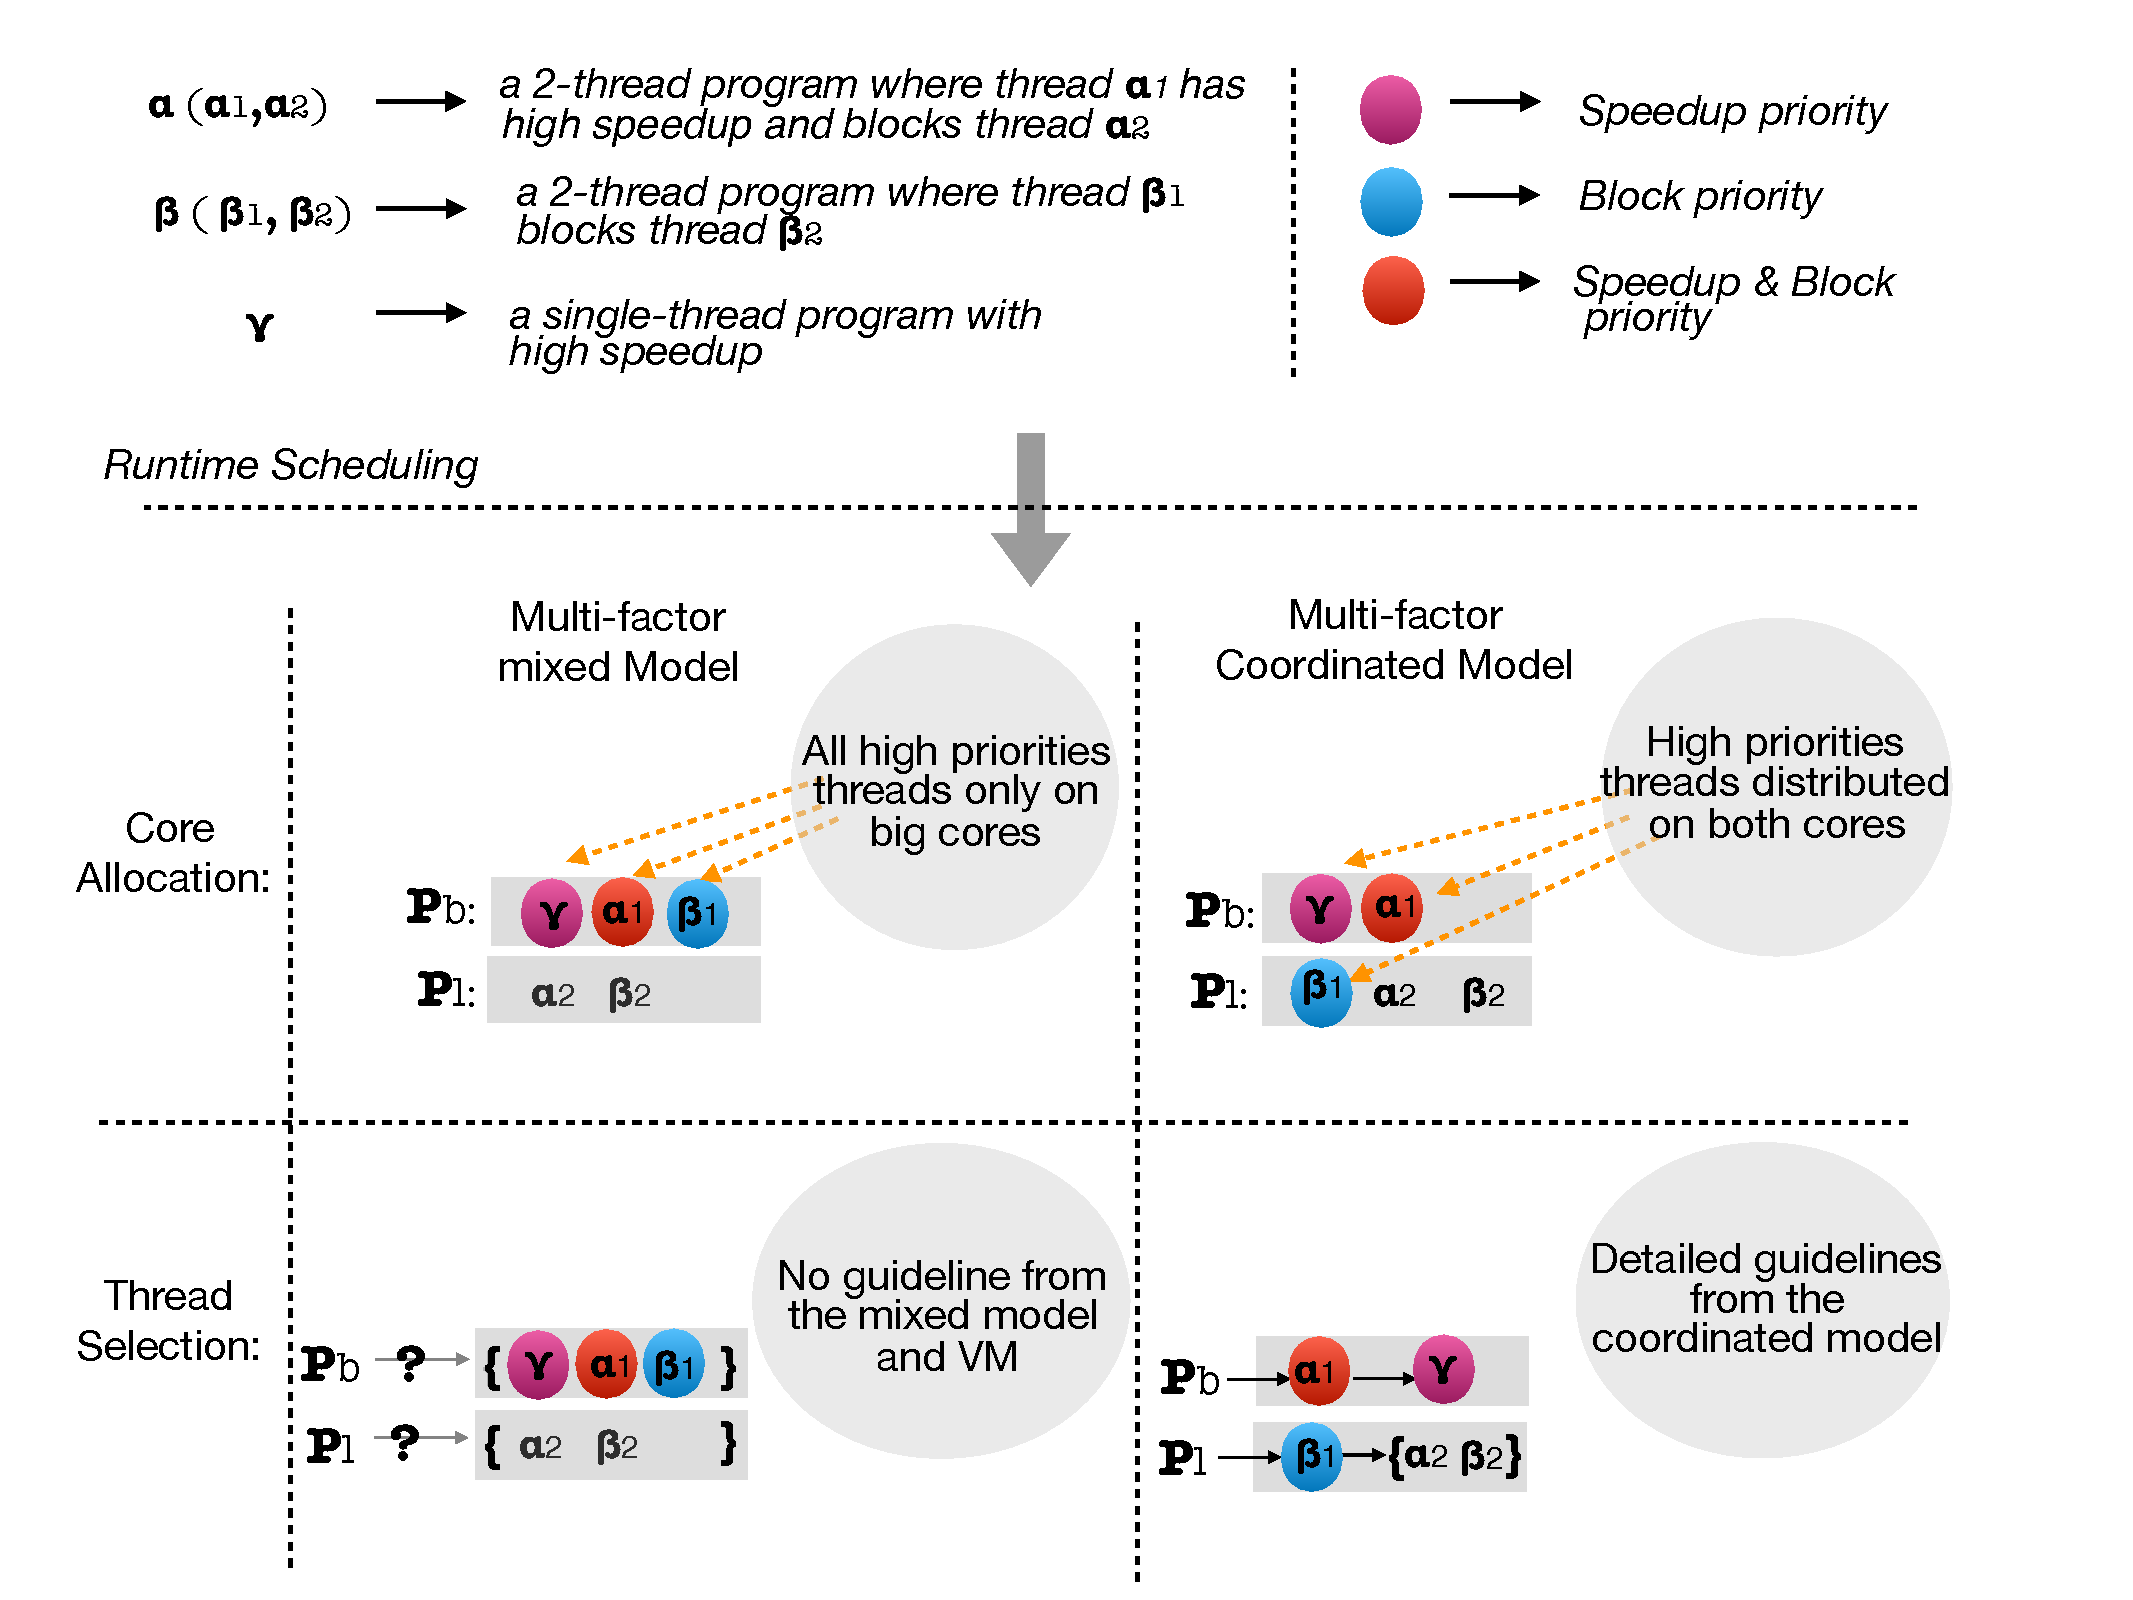
\includegraphics[scale = 0.25]{figures/me.pdf}
\caption{Motivating Example: Multi-threaded multiprogrammed workload on asymmetric multicore processors with one big core $P_b$ and one little core $P_l$. Controlling only core affinity results in suboptimal scheduling decisions.}
\label{me}
\end{figure} 

In this paper, we introduce COLAB, an OS scheduling policy for asymmetric multicore processors that makes coordinated decisions targetting all three main factors in thread scheduling - core sensitivity, thread criticallity and fairness. Our scheduler uses three collaborating heuristics to drive decisions about mapping threads to cores, each of the heuristics foucing primarly on optimisation of one of the factors. Collectively, these multi-factor heuristics result in better thread schedules compared to the Linux and WASH schedulers, therefore improving both performance and energy consumption. %ing decisions.
%We integrated COLAB in the Linux scheduler module, replacing the default CFS policy for all application threads.

The main contributions of our work are:
\begin{itemize}
\item  We present the design of a novel COLAB AMP-aware OS scheduler that targets general multi-threaded multiprogrammed workloads. The scheduler is based on a set of novel collaborative heuristics for addresing core sensitivity, thread criticality, fairness \emph{and} energy efficiency.
\item We present an implementation of the COLAB scheduler both on a real chip and in the simulation settings.
\item We evaluate the effectiveness of the COLAB scheduler on a range of standard workloads, demonstrating improvements of up to 25\% and 21\% (11\% and 5\% on the average) in the turnaround time compared to the Linux CFS and WASH schedulers in the GEM5 simulator and up to 27\% and 10\% performance gain (together with 5\% energy saving) compared to the ARM GTS and WASH scheduler on a real big.LITTLE development board.
  %
%\item Up to 25\% and 21\% lower turnaround time, 11\% and 5\% on average, compared to the default Linux CFS and WASH scheduler on GEM5. 
%\item Up to 27\% and 10\% performance gain, together with 5\% energy saving, compared to the default ARM GTS and WASH scheduler on HiHope Hikey 970.
\end{itemize}

\subsubsection*{Motivating Example} To demonstrate the problem, consider the example shown in Figure~\ref{me}, with an AMP system that has a high performance big core, $P_b$, and a low performance little core, $P_l$. Three applications are being executed - $\alpha$ and $\beta$ that have two threads, and $\gamma$ that is single threaded. 
The first thread of each application, $\alpha_1$ and $\beta_1$, blocks the second thread of their application, $\alpha_2$ and $\beta_2$, respectively. %$\gamma$ is a single-threaded application. 
$\alpha_1$ and $\gamma$ enjoy a high speedup when executed on $P_b$. WASH~\cite{jibaja2016portable}, the existing state-of-the-art multi-factor heuristic, would be inclined to assign the high speedup thread and the two blocking threads to the big core. The thread selector of $P_b$ has no information about the criticality of the threads assigned to it, so the order of execution depends on the underlying Linux scheduler.
A much better solution is possible if we control both core allocation and thread selection in a coordinated, AMP-aware way. In this case, we map the two threads that benefit the most from the big core, $\gamma$ and $\alpha_1$, to $P_b$, while we map the other bottleneck thread, $\beta_1$, to $P_l$. This will not impact the overall performance of $\beta$. The thread selector knows $\beta_1$ is a bottleneck thread and executes it immediately. So, what we lose in execution speed for $\beta_1$, we gain in not having to wait for CPU time. Similarly, this coordinated policy guarantees that $\alpha_1$ will be given priority over $\gamma$. 

%Based on the multi-factor mixed model \cite{jibaja2016portable}, either the high speedup thread ($\gamma$) or blocking threads ($\alpha_1,\beta_1$) will have affinity on $P_b$ -{\it local-optimal decision}. When the thread selector on $P_b$ is invoked, no more guideline can be obtained from the thread affinity provided by the mixed model - {\it loss of information with mixed priority}. Instead, a better solution can be provided in a multi-factor decentralized model by only mapping the two high speedup threads ($\gamma,\alpha_1$) to $P_b$ and keeping the other blocking thread $\beta_1$ in $P_l$ - {\it global-aware decision}. Then the thread selector invoked by both $P_b$ and $P_l$ guided through the blocking priority, will select and accelerate bottleneck threads $\alpha_1,\beta_1$ locally and simultaneously without waiting each other - {\it sufficient information with precise priority}.  

%both of them will get high priority and be affiliated on the big core. Thus, some of those high priority threads need to be waited in the runqueue of $p_b$. Further, when $p_b$ is ready to select the next task, it may select a $t_s$ first instead of a $t_b$ as the original bottleneck priority has lost after setup its affinity. In brief, the core allocator made the first {\it selfish} greedy decision to enqueue those high priority threads on big core without leaving a better solution space for thread selector. Second, the thread selector lose original information and cannot guarantee to make a good decision. With efficient preemption mechanism, $p_l$ can select a $t_b$ even from $p_b$'s runqueue, but this leads to additional overhead from migration. If the core allocator and thread selector can be collaborated, a trivial better solution in this example can be $p_b$ running \{$t_s \cap t_b$\} whilst $p_l$ running \{$t_b$\}. 

%The first problem is obvious as in runtime scheduling, every change in a current decision will influence the future solution space and there is no way to predict it especially for asymmetric multicore processors with multiple multi-thread workloads.  
%To demonstrate the second problem, scheduling a ready thread from a run-queue in big core to be executed in a ready little core can result in an optimal solution from a greedy point of view, or we say a {\it current} optimal solution. But if this thread will only run on the little core for a tidy bit of time and then move back to a big core by preemption when the big core is ready, the overall runtime overhead from additional migrations may totally defeat the benefit from the hard and useless work on the little core. A high level motivating example is shown in Fig \ref{mt}, where $\mathcal{T}$ is a high priority thread which just ranked in the second position under the current running thread on big core's run-queue. By global scheduling, a ready little core will decide to run this high priority thread $\mathcal{T}$ and migrate it from big core's run-queue. While the problem happens if the big core finish its current thread right after the migration issued by the little core, as the big core will decide to run $\mathcal{T}$ and move it back by preemption. Those frequent runtime selections and migrations do lower the performance in this case.

%We evaluated our policy on multiple big.LITTLE-like simulated systems running 36 distinct workloads, each workload being a random selection of PARSEC3.0, SPLASH2, and SPEC CPU2006 benchmarks. 
%In almost all cases, COLAB was able to improve both turnaround time and throughput compared to the state-of-the-art and the Linux default. In the best case, turnaround time was 25\% less under our policy than under WASH and CFS.
%In brief, our proposed framework equipped with a multi-factor {\it decentralized} model - different runtime factors are distributed to be mainly addressed by different functional units of the scheduler, including core allocator, thread selector and preemption trigger. Decisions in each functional unit are directly guided by priorities from sufficient runtime without losing information through a mixed central model. Those decisions only aim to benefit each of their targeting factors and avoid making trouble for each other, so neither greedy nor local-optimal from a multi-factor point of view. Then all those sub-decisions from different functional units in scheduler dynamically collaborate together to result in overall smarter scheduling decisions during runtime. 
%The remainder of this paper is presented as follows: Section 2 describes the background and related work. Section 3 presents our multi-factor collaborative model. We describe its implementation and analyze its operation in Section 4. We evaluate the scheduling police in Section 5, and we summarize and conclude the paper in Section 6.  

\section{Background and Related Work}
\label{rw}

\begin{table}[htbp]
  \caption{Qualitative Analysis on Related Work}
  \begin{center}
  \label{rwt}
  \scalebox{1.0}{
   \begin{tabular}{p{2.5cm} p{0.95cm} p{0.95cm} p{0.95cm} p{1.05cm}}
   \hline
     %\toprule[1pt]
     Approaches&Core Sens.&Fair- ness&Bottle- neck&Collabo- rative\\
     %\toprule[1pt]
     \hline
    Kumar, et al \cite{kumar2004single} &$\checkmark$&&&\\
    Li, et al \cite{li2009efficient}&&$\checkmark$&&\\
    Suleman, et al. \cite{suleman2009accelerating}&&&$\checkmark$&\\
    Saez, et al. \cite{saez2012leveraging}&$\checkmark$&$\checkmark$&&\\
    Craeynest, et al. \cite{van2013fairness}&$\checkmark$&$\checkmark$&&\\
    Cao, et al. \cite{cao2012yin}&$\checkmark$&&&\\
    Joao, et al \cite{joao2013utility}&$\checkmark$&&$\checkmark$&\\
    ARM \cite{jeff2013big}&&&$\checkmark$&\\
    Kim, et al \cite{kim2018exploring}&$\checkmark$&$\checkmark$&\\
    Jibaja, et al \cite{jibaja2016portable}&$\checkmark$&$\checkmark$&$\checkmark$\\
    \textbf{COLAB}&$\checkmark$&$\checkmark$&$\checkmark$&$\checkmark$\\
    \hline    
%\bottomrule
  \end{tabular}}
  \end{center}
\end{table}

Single-ISA heterogeneous processors allow for more efficient processing by using the right kind of core for each workload, while still relying on a single contract between hardware and software~\cite{kumar2004single,kumar2003single}. The only problem is deciding what "the right kind of core" is. For general purpose systems, where the mix of applications sharing the computational resources is not known at design time and changes rapidly, the optimal assignment of threads cannot be made statically. A scheduler needs to makes this decision at runtime.

The most direct approach, \emph{core sensitivity}, assigns threads to cores where they will experience the highest speedup. At its simplest, this might mean measuring the number of committed instructions per second on all core types and choosing the highest. In most cases though, this is inefficient. Existing approaches use performance models to predict the speedup from moving a thread to another core without having to execute the thread on that core. They first measure certain aspects of the thread's execution on its current core, \emph{ILP} and \emph{LLC miss rates} in Saez et al.~\cite{saez2012leveraging}, \emph{CPI stack}, \emph{ILP}, and \emph{MLP} in Craeynest et al.~\cite{van2012scheduling}, empirically selected performance counters in Jibaja et al~\cite{jibaja2016portable}. Then they use the performance model to estimate the effect of moving the thread elsewhere. The threads most sensitive to their placement are assigned to their preferred core type, the rest are assigned to any type of core.

Whole-program performance depends not only on accelerating core sensitive threads but also on accelerating the threads that slow down the program, the \emph{bottleneck and critical threads}. For example, previous work has shown the benefit from accelerating Amdahl's serial bottlenecks~\cite{Kumar:2005:HCM:1100859.1100890} and critical code sections~\cite{suleman2009accelerating}. Joao et al.~\cite{joao2012bottleneck,joao2013utility} further showed that functions that cause threads to wait above a certain threshold should be accelerated. Jibaja et al.~\cite{jibaja2016portable} similarly proposed finding bottleneck Java threads by measuring waiting time on contended locks.

On top of accelerating core sensitive and bottleneck threads, a general purpose AMP scheduler needs to \emph{maintain fairness}, that is to balance the processing resources given to each thread and process when they have to share these resources. Traditional fair schedulers balance only processing time, assuming that time is equally important on all cores. This is not true for AMPs. Li et al~\cite{li2007efficient} introduced some sense of fairness by loading each core proportionally to its processing power. Craeynest et al.~\cite{van2013fairness} instead proposed an \emph{equal progress} scheduler. It uses a performance model to express the progress of every thread in terms of the time required for the same progress on the small core. The scheduler then prioritizes threads so that the small core equivalent time of all threads is the same. Other heuristics have tried to maximize fairness on AMPs~\cite{zahedi2018amdahl,wang2016rebudget,kim2018exploring} but for restricted scenarios.

Only a small number of schedulers are designed to handle the general case of multi-threaded multi-programmed workloads. ARM Global Task Scheduler (GTS)~\cite{jeff2013big} focuses on energy efficiency. Threads run on low power cores unless they are servicing interrupts or have a high load. Core sensitivity is not a concern, while bottlenecks are only accelerated when they happen to be caused by high load threads. Kim and Huh~\cite{kim2018exploring} focuses only on core sensitivity and fairness. Inter-thread communication is not a concern. WASH~\cite{jibaja2016portable} is to our knowledge the only existing scheduler that handles core sensitivity, bottlenecks, and maintains fairness. Still, it is limited to only controlling affinity and requires the OS scheduler to independently dispatch threads to cores. As we see later, this lack of collaboration between the two subsystems is sub-optimal. In the rest of this paper, we use a WASH-like implementation that relies on the baseline Linux scheduler as our state-of-the-art. A qualitative comparison of the related work is shown in Table \ref{rwt}.
\section{System Overview}
We provide a high level COLAB system overview as shown in Figure~\ref{figure:f1}. The system is divided by an runtime scheduling process and an offline modelling processes. The runtime scheduler is built inside OS kernel and composed by a core allocator to handle fairness and core sensitivity, a thread selector to achieve bottleneck acceleration and machine learning based runtime models, which predicate speedup and power consumption of threads on heterogeneous cores. The offline modelling processing is applied to construct runtime models by offline training. 

The main novelty of COLAB scheduler is that it can handle multiple runtime factors (core sensitivity, bottleneck acceleration and fairness) in a collaborative way to achieve high system performance and energy efficiency. To easy understand the runtime collaboration, we first analyze the performance impact of multiple runtime factors and their relationship with different scheduler components. We then discuss how to build the scheduler which addresses these performance problems in a coordinated way. After that, we present the detailed design and implementation of the proposed COLAB scheduler, beginning from the supporting offline modelling process to the runtime scheduling process. 

\begin{figure}
\centering
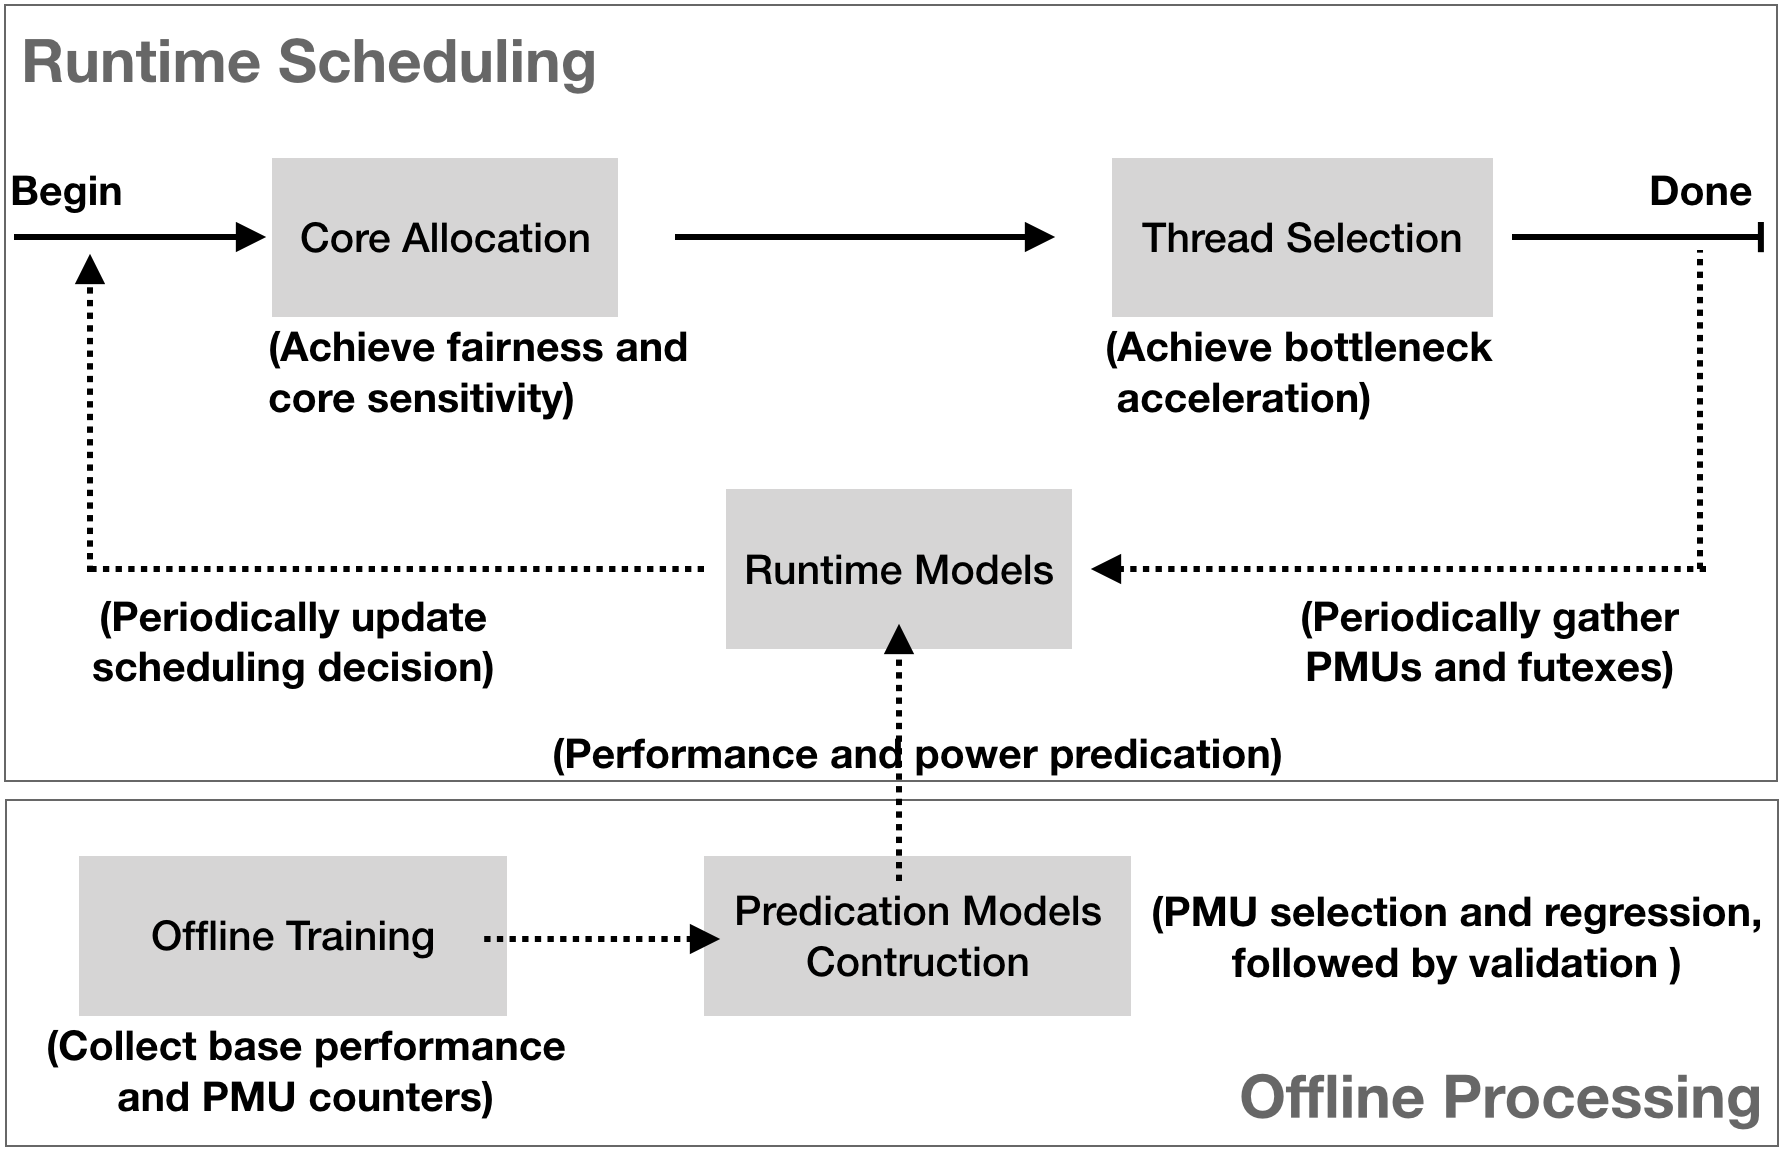
\includegraphics[scale=0.27]{figures/overview.png}
\caption{System Overview}
\label{figure:f1}
\end{figure} 

\begin{figure}
\centering
\includegraphics[scale=0.4]{figures/mfa.pdf}
\caption{A diagram of Performance Factors and Relationships with Scheduling Functions}
\label{figure:f11}
\end{figure} 

\section{Runtime Analysis}
Figure~\ref{figure:f11} shows the relationship between runtime performance factors and the scheduler components that address them. 
In order to achieve runtime collaboration, both the core allocator and the thread selector share information and account for all measured performance factors, including core sensitivity, bottleneck acceleration and fairness. In this section, we first analyse the relationships and then discuss the collaboration. 
% as illustrated below:
%We describe them below by discussing each element. 
%\begin{itemize}
\subsection{Runtime Factors Analysis}
\textbf{\textit{Core Allocator:}}
AMP-aware Core allocators are mainly directed by the core sensitivity factor -- migrating a high speedup thread (with a large differential between big and little core execution time) from  a little core to execute on a big core will generally provide more benefit than migrating a low speedup thread. 
However this heuristic is overly simplistic. Issues are revealed when the bottleneck factor is considered simultaneously on multiprogrammed workloads. Previous approaches \cite{jibaja2016portable} simply combine the calculation from  bottleneck acceleration and predicted speedup together, but this can result in suboptimal scheduling decisions -- both locking threads and high speedup threads may be accumulating in the runqueues of big cores as described in the motivating example. More intelligent core allocation decisions can be made by avoiding a simple combination of bottleneck acceleration and speedup -- the overall schedule can benefit from a more collaborative execution environment where big cores focus on high speedup bottleneck threads, and little cores handle other low speedup bottlenecked threads without additional migration.
%migrating threads with a lower predicted speedup, but which are blocking other threads.  
Furthermore, core allocators attempt to achieve relative fairness on AMPs by efficiently sharing heterogeneous hardware and avoiding idle resources as much as possible. 
Simply mapping ready threads uniformly between different type of cores can not achieve true load-balancing -- the number of ready threads prioritized on different type of core is different and thus a hierarchical allocation should be applied to guarantee overall fairness, which avoids the need to frequently migrate threads to empty runqueues. 

\textbf{\textit{Thread Selector:}}
The \textit{thread selector} makes the final decisions on which thread will be executed during runtime. It is usually the responsibility of the thread selector to avoid bottlenecking by thread blocking. In a multi-thread multiprogrammed environment, multiple bottleneck threads from different programs may need to be accelerated simultaneously with constrained hardware resources. Instead of simply detecting the bottleneck threads and assigning all of them to big cores, as previous bottleneck acceleration schedulers do~\cite{jibaja2016portable,joao2013utility,joao2012bottleneck}, the thread selector needs to make collaborative decisions -- ideally, both big cores and little cores select bottlenecks to run simultaneously.
Core sensitivity is usually unimportant to the thread selector -- whether a thread can enjoy a high speedup from a big core compared with a little core is unrelated to which runqueue it is on, or came from. Therefore the thread selector should separate thread priority caused by core sensitivity and solely base decisions on bottleneck acceleration. One exception is that when the runqueue of a big core is empty and the thread selector is invoked -- the speedup factors from core sensitivity of ready threads should be considered only in this case. Big cores may even preempt the execution of little cores when necessary.  
The final concern of thread selector concerns fairness. Scaling time slice of threads by updating the time interval of thread selector has been shown to efficiently guarantee the equal progress \cite{van2013fairness} in multi-threaded single-program workloads and achieve fairness. 
%In single-threaded multiprogrammed scenarios, complicated fairness formulation \cite{kim2018exploring} has been proposed to guide the thread selector for more precise decisions. 
Problems occur when targeting multi-threaded multi-programmed workloads. Simply keeping a thread-level equal progress is not enough to guarantee the multi-application level fairness -- the thread selector should ensure the whole workload is in equal progress without penalizing any individual application. In fact,  multi-bottleneck acceleration by both big and little cores does provide an opportunity for this - the thread selector makes the best attempt to keep fairness on all applications by accelerating bottlenecks from all of them and as soon as possible.


%\textbf{\textit{Fairness:}} Fairness is critical for system performance. A good schedule achieving relative fairness on AMPs should efficiently share heterogeneous hardware and avoid idle resource as much as possible. To achieve the expected relative equal-progress between threads and load-balancing between cores, the core allocator should map ready threads relative uniformly,avoiding the need to frequently migrate threads to empty runqueues. The design of the preemption triggering mechanism  also affects fairness, as it determines the maximum length of a time slice.


%The preemption triggering mechanism of thread selector is also related with the fairness factor as it determines the slice of a task running each time - a thread currently running on big cores should have relatively shorter time slice against its running on little cores to result in similar progress.
%The preemption should be triggered and the thread selector should be invoked less frequent on little cores than on big cores     

%\textbf{\textit{Core Sensitivity:}} Previous approaches considered core sensitivity and predicated speedup of threads but can result in poor scheduling decisions on multi-threaded, multi-programmed co-execution workloads. Selecting threads simply by predicted speedup on asymmetric cores may not lead to a overall good solution --  for instance, a high speedup thread detected on a little core could benefit by migrating to a big core, but is not blocking a significant number of other threads. The overall schedule can benefit more by migrating threads with a lower predicted speedup, but which are blocking other threads. Thus, we find priority from core sensitivity should be mainly addressed by the core allocator and be independent from the thread selector. 
%For instance, a thread with high predicted speedup should have more opportunities to be allocated and executed on a high-performance big core compared to a low predicted speedup thread. Higher speedup and more sensitive on big core does not indicate any {\it emergency} to execute this threads amount all other ready threads during the runtime. 
%No priority should be given to high-speedup threads for a thread selector, only if in a special case when a big core finishes its current task with an empty runqueue and all other big cores hold empty runqueue as well - so it needs to globally select a ready thread from a runqueue of little core and then relative higher speedup threads are better candidates. This special case won't even appear in large-scale parallel workloads scenarios where the number of co-executing programs is at least greater than the number of cores - there will always be waiting threads in a big core's runqueue based on fairness core allocation as no data-dependence between threads from different programs. 

%\textbf{\textit{Bottleneck Acceleration:}} Threads from multi-threaded programs holding contended locks and blocking other parallel threads should be identified as bottleneck and be executed as soon as possible. In large-scale workloads scenarios where multi-threaded multi-program are co-executing on limited AMPs resources and multiple blocking threads waiting to be executed simultaneously, the thread selector should take the main duty to select those bottlenecks and run the corresponding critical code segments in an efficient way without confused by the priority from core sensitivity. In detail, the thread selector triggered by big cores should always give higher priorities for a thread with higher blocking level against another thread with higher speedup level and lower bottleneck. It may preempt the running threads on little cores to accelerate them when suited. The thread selector triggered by little cores should also intend to select relative high blocking threads and accelerate them locally first, instead of trivially migrating it to big cores and waiting to be actual accelerated there.  

\begin{figure}
\centering
\includegraphics[scale=0.5]{figures/COLAB_M.pdf}
\caption{Coordinated Runtime Scheduling by Multi-factor Collaboration}
\label{figure:f2}
\end{figure} 

\begin{figure*}
\centering
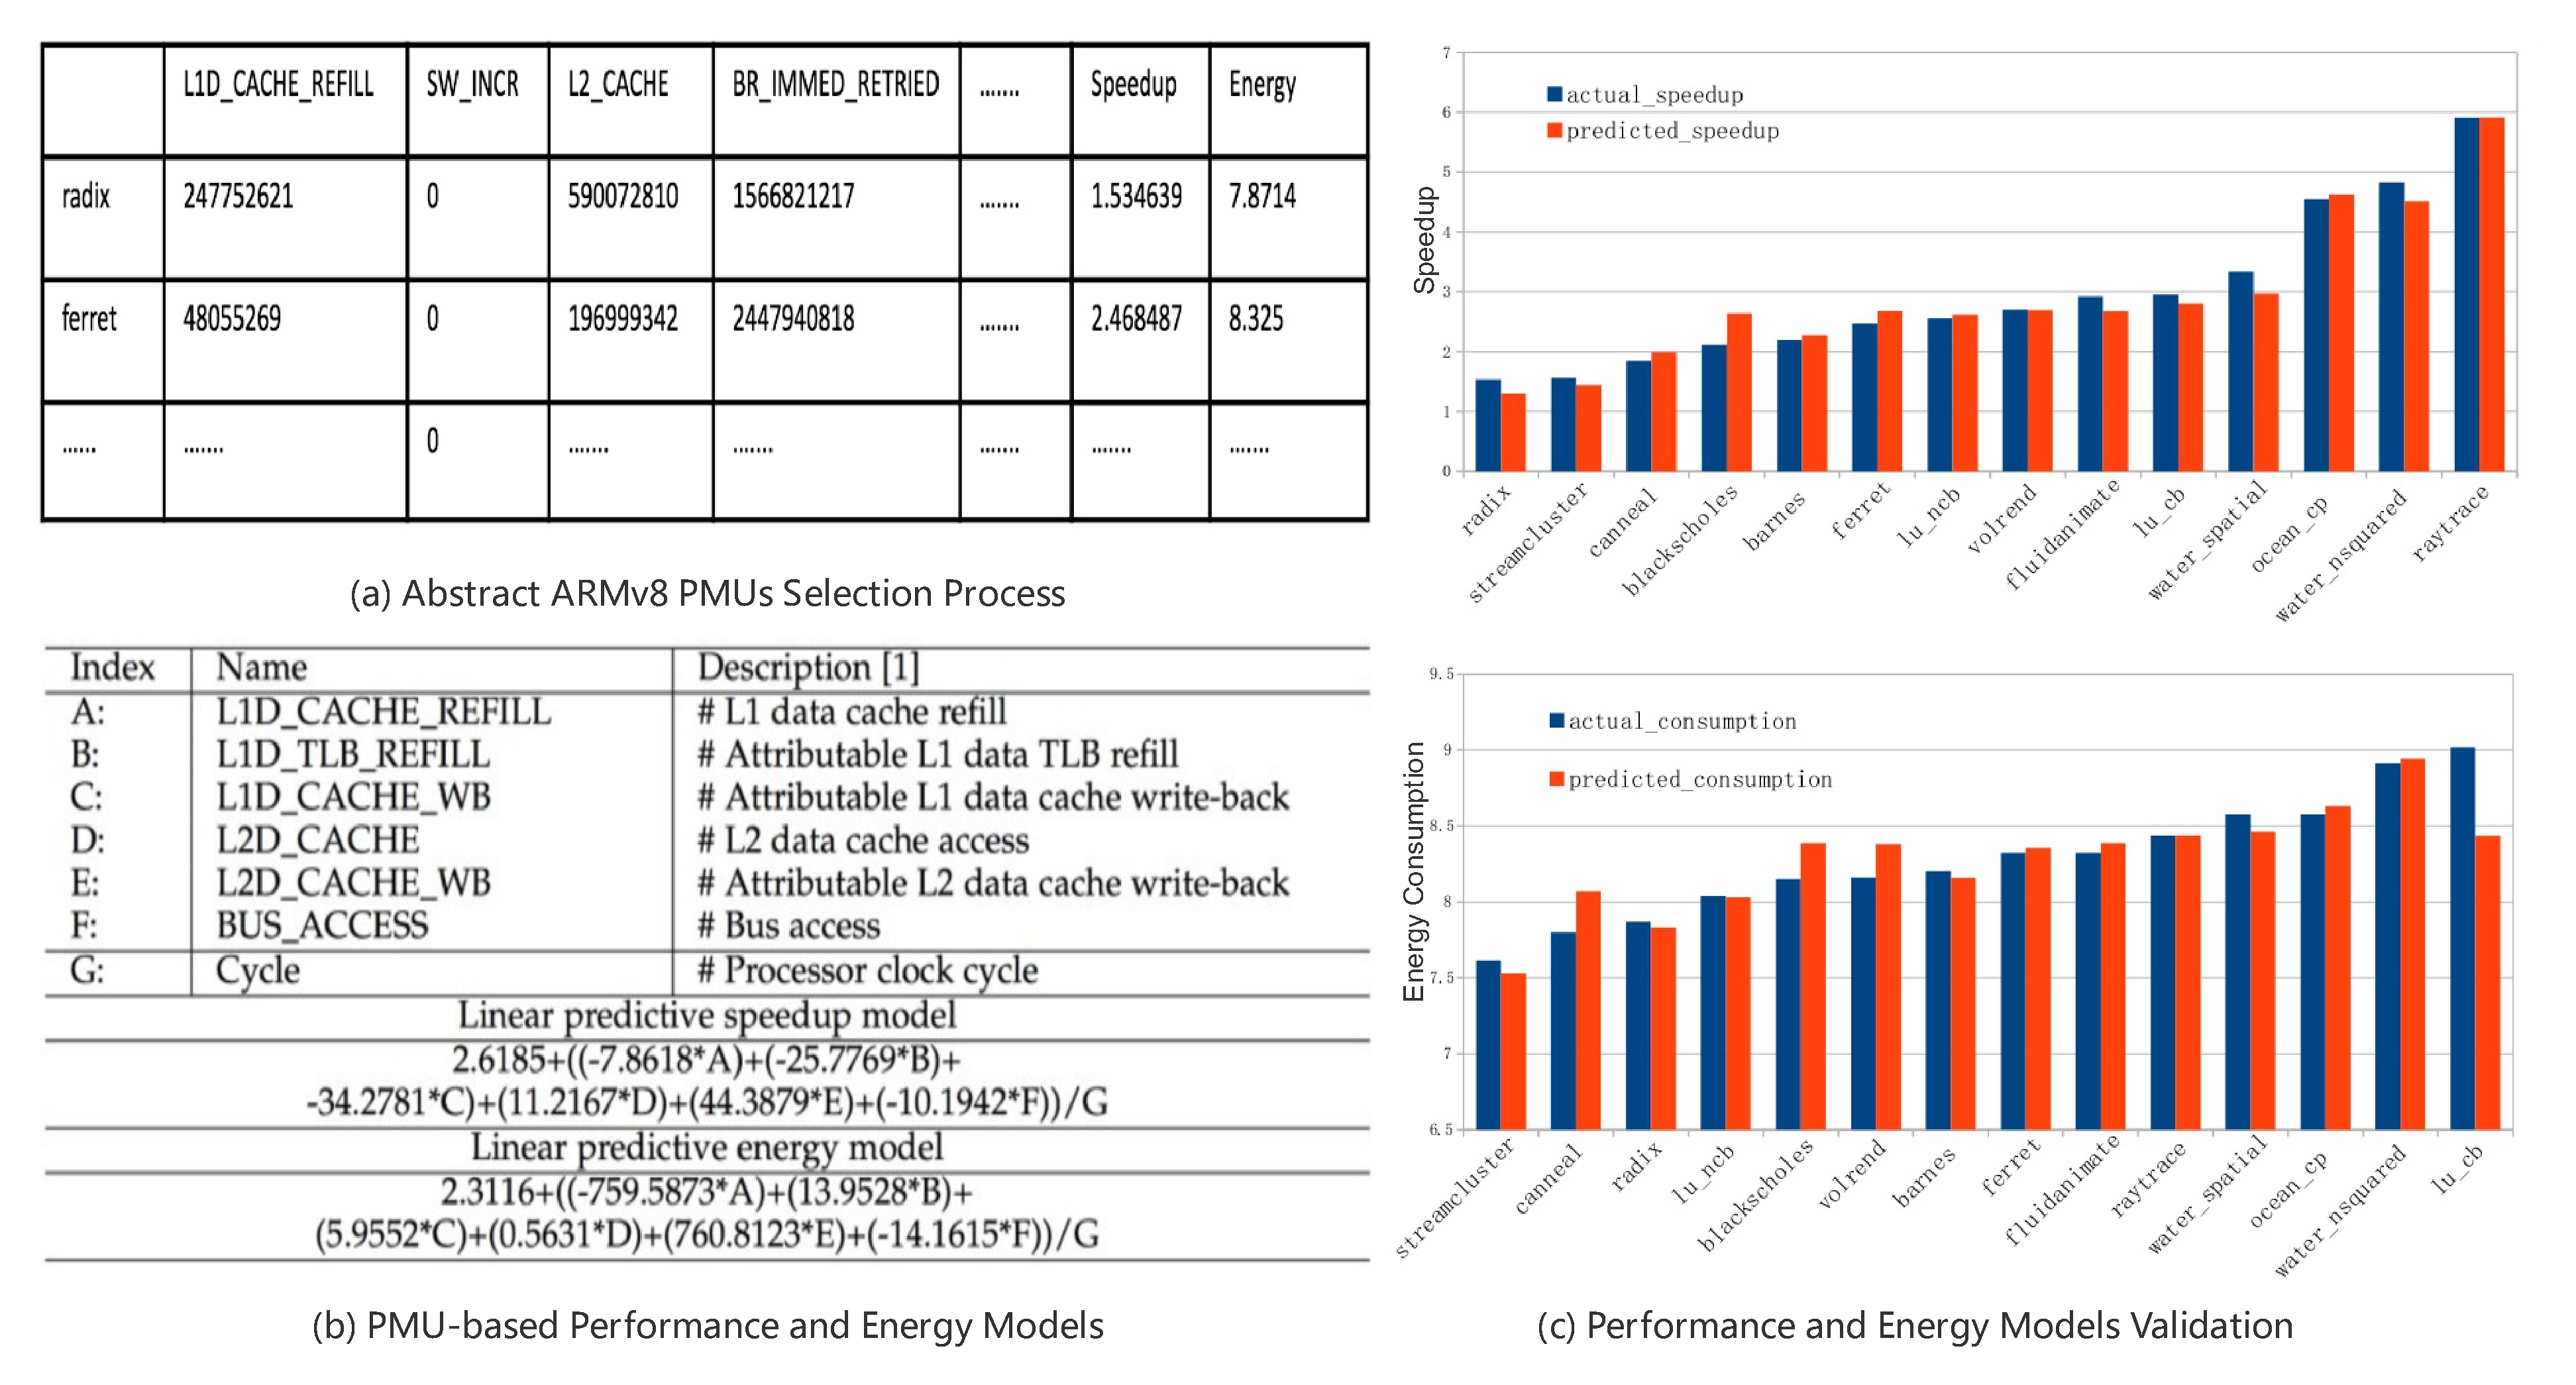
\includegraphics[scale=0.25]{figures/arm_model.pdf}
\caption{ARMv8 Performance and Energy Modelling. \fixme{PP: This looks like a screenshot.}}
\label{arm_model}
\end{figure*}
\subsection{Runtime Collaboration}
To address the problems detailed above, we designed a coordinated multi-factor scheduler in which the core allocator and the thread selector collaborate to achieve high performance and high fairness, when compared to %the state-of-the-art mixed multi-factor evaluator in 
WASH \cite{jibaja2016portable}.
% VJ " We mentioned quite a few times already that WASH is state-of-the-art mixed multi-factor thing...
%While the way we define whether a thread's relative speedup value is high or low is similar as in WASH based on hardware configuration - if we have same number of big and little cores, then we rank all ready threads based on its relative speedup and view the first half as high speedup value. 
The flowchart of our model is shown in Figure~\ref{figure:f2}. 
Collaboration is facilitated by periodically labeling ready threads in two different categories, based on runtime models of speedup prediction and bottleneck identification: 
%\begin{itemize}

\textbf{\textit{Labels for Core Allocation:}}
Threads with high predicted speedup between big and little cores will be labeled as high priority on big cores. Threads with both low predicted speedup and blocking levels -- non-critical threads -- will obtain high priority on little cores (and low priority on big cores). Remaining threads obtain equal priority on either big or little cores -- these threads can then be allocated freely to balance the load of cores.

\textbf{\textit{Labels for Thread Selection:}}
Threads with high blocking level will be labeled as high priority on local thread selection. The same priority will be given on these blocking threads whether the issuing cores are big or little, so the labels of thread selection do not distinguish the type of cores.The label nevertheless records the type of the current core -- threads always have priority to be selected by the same type of cores if there exists a core of the same type with an empty runqueue. Running threads on little cores are also labeled as they may be preempted to migrate and execute on big cores when suited, but running threads will never have priority over waiting ready threads. 


%The thread labels should be not only be based on the relative ranking between threads, but also on boundary conditions targeting different hardware resource and experimental environments. 
%We setup empirical boundaries for speedup and blocking: (1) No thread is ranked as high-speedup if its predicted speedup value is less than an empirical architecture-specific boundary, calculated using relative frequency between big and little cores. 

%For instance, if the big cores' frequency is 2x faster than the little cores and ready threads get around 1.5x predicted speedup, this likely means threads haven't be executed long enough to get a more precise speedup value and we should not bind or migrate any thread at this step. 
%(2) Threads will not be ranked as high-blocking if the rate of their blocking time and life time are less than a relative boundary or the life time of them are less than a starting point - For instance, no thread should be ranked as relative high-blocking during the initial time periods of experiments.   
%It is mainly benefit in a mixed workloads scenario where we co-execute single and multi-threaded multiprogrammed - a non-computing-intensive code segment from a single thread program can neither enjoy good performance gain on big cores nor block others. So we should better keep it in a little core and let other blocking threads to be executed before it. 

After the labeling process, fairness, core sensitivity and bottleneck acceleration are represented by labels on threads can be handled by either the core allocator or the thread selector or both together. Based on this coordinated model, the core allocator and thread selector handle different priorities queues from the set of ready threads -- their decisions are not greedy on a mixed multi-factor ranking like WASH, rather provide a collaborative schedule.
Another important issue handled by the collaborative multi-factor model is to ensure equal-progress of threads as shown in the upper-right corner of Figure~\ref{figure:f2}. Instead of interfering with the priority and decisions of thread selection, we achieve equal progress in threads by our scaled time slice approach, based on the predicted speedup value of threads running on big cores. The slices of threads on big cores are relative shorter than on little cores. The thread selection function is triggered more often to swap executing threads on big cores, which guarantees the relative equal-progress of threads executed on all cores.
The runtime model periodically extracts the performance counters, which represents the current execution environment of multi-threaded multi-programmed workloads on the AMPs. The model then computes the updated runtime factors, including the predicated speedup value and blocking counts. This information is attached to the threads and reported back to the multi-factor labeler for next round. We present our runtime implementations in the section below. 



\section{COLAB Scheduler Design and Implementation}
This section explores the design and implementation of COLAB inside the Linux kernel. We describe our performance and energy models, our modifications of the kernel to support COLAB, and finally the scheduling algorithm itself, including its runtime overheads.

\subsection{Offline Performance and Energy Modelling}
The decisions of our Core Allocator are primarily driven by core sensitivity. To predict whether a thread is core sensitive or not, we develop a machine learned performance model similar to the ones used in previous works in this area~\cite{van2013fairness,jibaja2016portable,saez2012leveraging}. The model is constructed offline once and is kept purposefully simple, a linear regression model with seven parameters, to minimize the runtime overhead. 

%Predicting the relative speedup of each thread between different core types is central for any scheduler targeting AMPs. Our prediction uses a machine learning approach by offline training and online estimation as shown in Figure~\ref{arm_model}. This is a common approach in previous works \cite{van2013fairness,jibaja2016portable,saez2012leveraging}. 

%The abstract offline PMU selection process is shown in Fig.~\ref{arm_model}(a). 

The training data we collect are execution time, energy consumption, and event counts from all performance monitor units (PMU). We run each training application in isolation under two different configurations, first on the little core cluster and then the big core cluster of our evaluation system. Since we only have access to seven PMUs at any given moment, we repeatedly execute each application while collecting different PMUs, until we have reliable information for all of them. At the end of this process, we have performance event counts, performance scaling between big and little cores, and energy scaling between big and little cores for 14 programs. Through Principal Component Analysis (PCA)~\cite{witten2016data}, we select the six performance events that correlate the most with performance and energy scaling. Finally, we use linear regression to associate the six selected events, as well as the clock cycle count, with performance and energy scaling. This results in the two models shown in Table~\ref{arm_model}(b).

%To construct the training set, we run all applications in single-program mode with two symmetric configurations, using either only little cores (4 Cortex-A53) or only big cores (4 Cortex-A73). We first record common performance monitor units (PMUs) used for both Cortex-A73 and Cortex-A53, together with each thread's relative speedup and energy consumption. We ignore the PMUs for which their value keep to be zero, such as \texttt{SW\_INCR} (Instruction architecturally executed, Condition code check pass, software increment). 

%Since the targeting ARMv8 architecture only contains 7 hardware register to support PMUs, we do not have access to all PMUs simultaneously. We apply Principal Component Analysis (PCA) technique \cite{witten2016data} to select a 6-PMU-combination with the largest effect on speedup and power modeling. For example, it is easy to know that the performance and energy will be more dominated by the total data movement than some branch behaviours. As a result, although \texttt{BR\_IMMED\_RETIRED} is a meaningful PMU which counts all immediate branch instructions that are architecturally executed, but it is not selected after the PCA process as there are more important PMUs such as \texttt{L1D\_CACHE\_REFILL} (L1 data cache refill) and \texttt{L2\_CACHE} (L2 data cache access). We then normalize all counters to the number of clock cycles and use linear regression to build the final model. The clock cycle number is stable recorded by a specialized register on the test ARMv8 development board. The trained PMU-based performance and energy models are shown in Table~\ref{arm_model}(b).

We validate the accuracy of our trained models on each benchmark as shown in Fig.~\ref{arm_model}(c). The average error across all benchmarks is around 7\% for performance scaling prediction and around 1.5\% for energy scaling prediction. \fixme{PP: Can we say something about why we are so wrong for lu\_cb?}


\begin{comment}
\begin{table}
  \caption{Selected GEM5 performance counters and the Speedup Model}
  \center
  \label{pca_gem5_sp}
   \scalebox{0.8}{
   \begin{tabular}{p{0.8cm} | p{4.8cm} | p {3.8cm} c c c}
  \hline
     Index&  Name& Description \cite{binkert2011gem5} \\
    \hline
     A: & fp\_regfile\_writes & \# integer regfile writes\\
     B: & fetch.Branches & \# branches encountered\\
     C: & rename.SQFullEvents & \# SQ-full blocks\\
     D: & quiesceCycles & \# interrupt waiting cycles\\
     E: & dcache.tags.tagsinuse & \# tags of dcache in use\\
     F: & fetch.IcacheWaitRetryStallCycles & \# MSHR-full stall cycles\\
     \hline
     G: & commit.committedInsts & \# instructions committed\\
     \hline
     \multicolumn{3}{c}{Linear predictive speedup model}\\
     \hline
    \multicolumn{3}{c}{2.6109+((0.0018*-0.185A)+(0.0259*0.187B)+}
    \\
    \multicolumn{3}{c}{(0.1047*0.194C)+(-0.023*0.238D)+(0.0492*-0.299E)+(-0.1388*-0.227F))/G}\\
 \hline
  \end{tabular}}
\end{table}
\end{comment}

\subsection{Runtime Supporting Techniques}
\textbf{\textit{Bottleneck Identification:}}
On modern Linux systems thread synchronization primitives are almost always implemented on top of kernel futexes, regardless of the threading library used. Futex-based mechanisms use a single atomic instruction in user space to acquire or release the futex, if it is uncontested. Otherwise, it calls the kernel which forces the thread to sleep or wakes up sleeping threads respectively.
This means that monitoring the blocking patterns between threads requires instrumenting only this interface. Right before an active thread starts waiting on a futex, in \texttt{futex\_wait\_queue\_me()} and \texttt{futex\_lock\_pi()}, we record the current time and store it in the thread's \texttt{task\_struct}. We mirror this with code right before a waiting task is woken up, in \texttt{wake\_futex()} and \texttt{wake\_futex\_pi()}. At this point we calculate the length of waiting time for the thread and we accumulate it in a field of the \texttt{task\_struct} of the thread releasing the futex. This enables us to measure the cumulative time each thread has caused other threads to wait. This is our thread criticality metric for the rest of the paper.

%We instrument this interface to monitor the blocking patterns between threads. This gives us a convenient single point for monitoring blocking patterns between threads. We first add code in \texttt{futex\_wait\_queue\_me()} and \texttt{futex\_lock\_pi()}, right before the active thread starts waiting on a futex. We record the current time and store it in the \texttt{task\_struct} of the thread. We then insert code in \texttt{wake\_futex()} and \texttt{wake\_futex\_pi()}, right before the waiting task is woken up by the thread releasing the futex. There we calculate the length of the waiting period and we accumulate it in the \texttt{task\_struct} of the thread releasing the futex. This way we are able to measure the cumulative time each thread has caused other threads to wait. We use this as our metric of thread criticality for the rest of the paper.

\textbf{\textit {Speedup based Scale-slice Preemption:}} The default preemption mechanism of Linux is triggered every time a new task in enqueued at which point it checks whether the virtual runtime {\it vruntime} of the incoming task is significantly lower than that of the running task. If this is the case, sharing the processing time fairly requires preempting the running task. While our approach keeps this mechanism intact, we modify vruntime so that equal vruntimes represent equal progress in an AMP system instead of just equal runtime. We do this in the default preemption function \texttt{wakeup\_preempt\_entity()}. If the triggering core is a big one, then the vruntime of the task is divided by the model predicted speedup for the task. This is equivalent to predicting the vruntime required to achieve the same progress on a little core.

%Although we implement our scheduler on Linux kernel by fully re-writing both the core allocator and thread selector, the underlying preemption mechanism of Linux is applying the virtual runtime {\it vruntime} in CFS with red-black tree data structure - whenever a new task is enqueued, a preemption wake-up function is invoked to check whether the new coming task should preempt the current task by computing the difference in vruntime and comparing with a boundary. 
%To achieve equal-progress on AMPs, threads running on different types of cores should have different time slices instead of trying to achieve complete fairness on time. We update the default preemption function \texttt{wakeup\_preempt\_entity()} in Linux. To ensure relative equal progress, we apply our runtime speedup model to update the vruntime of the task by dividing it by the its speedup value if the triggering core is a big core. %The ensures relative equal progress.

\subsection{Scheduling Algorithm Implementation}
\begin{algorithm}
\caption{COLAB: Collaborative Multi-factor Scheduler targeting Asymmetric Multicore Processors}
\label{alg:1}
\begin{algorithmic}[]
\STATE \textbf{\_core\_alloctor\_(thread\_struct\ $t$)}\{
%\FOR {$t : ready\_threads$}
%\IF {t->high\_speedup() \& t->high\_block()}
%\STATE \textbf{if} foo

%\IF {t.high\_speedup}
%\RETURN rr\_allocator\_(big\_cores)
%\ENDIF
\STATE \textbf{if} t.high\_speedup
\STATE \ \ \textbf{return} rr\_allocator\_(big\_cores)
\STATE \textbf{if} {t.low\_speedup \& t.low\_block}
\STATE \ \ \textbf{return} rr\_allocator\_(little\_cores)

\STATE \textbf{else return} rr\_allocator\_(cores) \}
\STATE
\STATE \textbf{\_thread\_selector\_(core\_struct\ $c$)}\{
%\IF {c->cur \& !(preempt_wakeup)}
\STATE \textbf{if}  !empty(c.rq)
\STATE \ \ \textbf{return} max\_block\_(c.rq)
\STATE \textbf{if} !empty(c.sched\_domain.rq)
\STATE \ \ \textbf{return} max\_block\_(c.sched\_domain.rq)
\STATE \textbf{if} c.cpu\_mask == big
%\FOR {t : little\_core->cur}
%\STATE candidates.enqueue(t)
%\IF {!empty(candidates)}
\STATE \ \ \textbf{return}  max\_block\_(c.sched\_domain\_little.cur)
%\ENDFOR
%\ENDIF
%\FOR {t : other\_little\_core->rq}
%\STATE candidates.enqueue(sorted\_speedup(t))
%\ENDFOR
%\IF {!empty(candidates)}
%\RETURN  max\_block\_(candidates)
%\ENDIF
%\ENDIF
%\FOR {t : other\_core->rq}
%\STATE candidates.enqueue(reversed\_speedup(t))
%\ENDFOR
\STATE \textbf{else return} idle \}
\end{algorithmic}
\end{algorithm}

\noindent
Our scheduling algorithm (see Alg.~\ref{alg:1}) is implemented by overriding the default task selector \texttt{pick\_next\_task\_fair()} and core allocator \texttt{select\_task\_rq\_fair()} in Linux kernel supported by the runtime factors. %The pseudo-code of our scheduling algorithm is shown in Alg. \ref{alg:1}. 
In line with standard Linux notation, we use $rq$ and $cur$ to represent runqueue and the current task of a core, respectively. We describe the two main functions followed by a energy-aware extension:

\textbf{\textit{Hierarchical Core Allocator:}}
When a spawned or woken thread is ready to be executed, the core allocator will be invoked to assign this thread to a core's runqueue. To achieve relative load balancing and consider the influence from the core sensitivity factor, we involve a hierarchical round-robin mechanism \texttt{rr\_allocator\_()}. Indicated by the speedup and blocking labels, threads are allocated to different core groups. Threads with high speedup will be round-robin assigned in big core clusters. Low speedup and low blocking threads will only be assigned in little core clusters. 
%A technical issue here is we need to distinguish threads which are part of a multi-thread program from from single-thread programs - these single-thread program threads will definitely not block others and may not have a high speedup but we should nevertheless not bind them to little cores. They can be easily detected by the allocator by checking whether there are ready threads whose group pid (t->tgid) equals to any others (line 5). 
Remaining ready threads (usually with average speedup level and little blocking) will be relatively equally allocated to both core types by \texttt{rr\_allocator\_()}. This final round-robin decision helps to keep both core clusters equally occupied and load balanced. 

\textbf{\textit{Biased-global Thread Selector:}}
The thread selector is based on the principle of accelerating the most critical/blocking thread as soon as possible. The selector always tries to choose a thread from the local runqueue first. When there are no ready threads and migration is beneficial, the core triggers the migration of a candidate thread waiting in another runqueue. The highest blocking thread will be selected.
To reduce the overhead of accessing state in other runqueues, we follow the same principle as the default Linux CFS scheduler, returning the best candidate thread from the local core group first.
Further, we allow a big core to select and preempt a running thread on a little core to accelerate it. Big cores are allowed to go idle only when there is no ready thread left - for instance, we do not allow a little core to preempt a big core's execution. 
%In summary, the thread selector can still access all other runqueues when necessary, but it is biased to access neighbouring ones first. 
The equal-progress for achieving fairness is addressed by the scale-slice preemption checker  -- we give each thread a maximum time slice relative to its expected performance on the asymmetric core.




\begin{figure*}
\centering
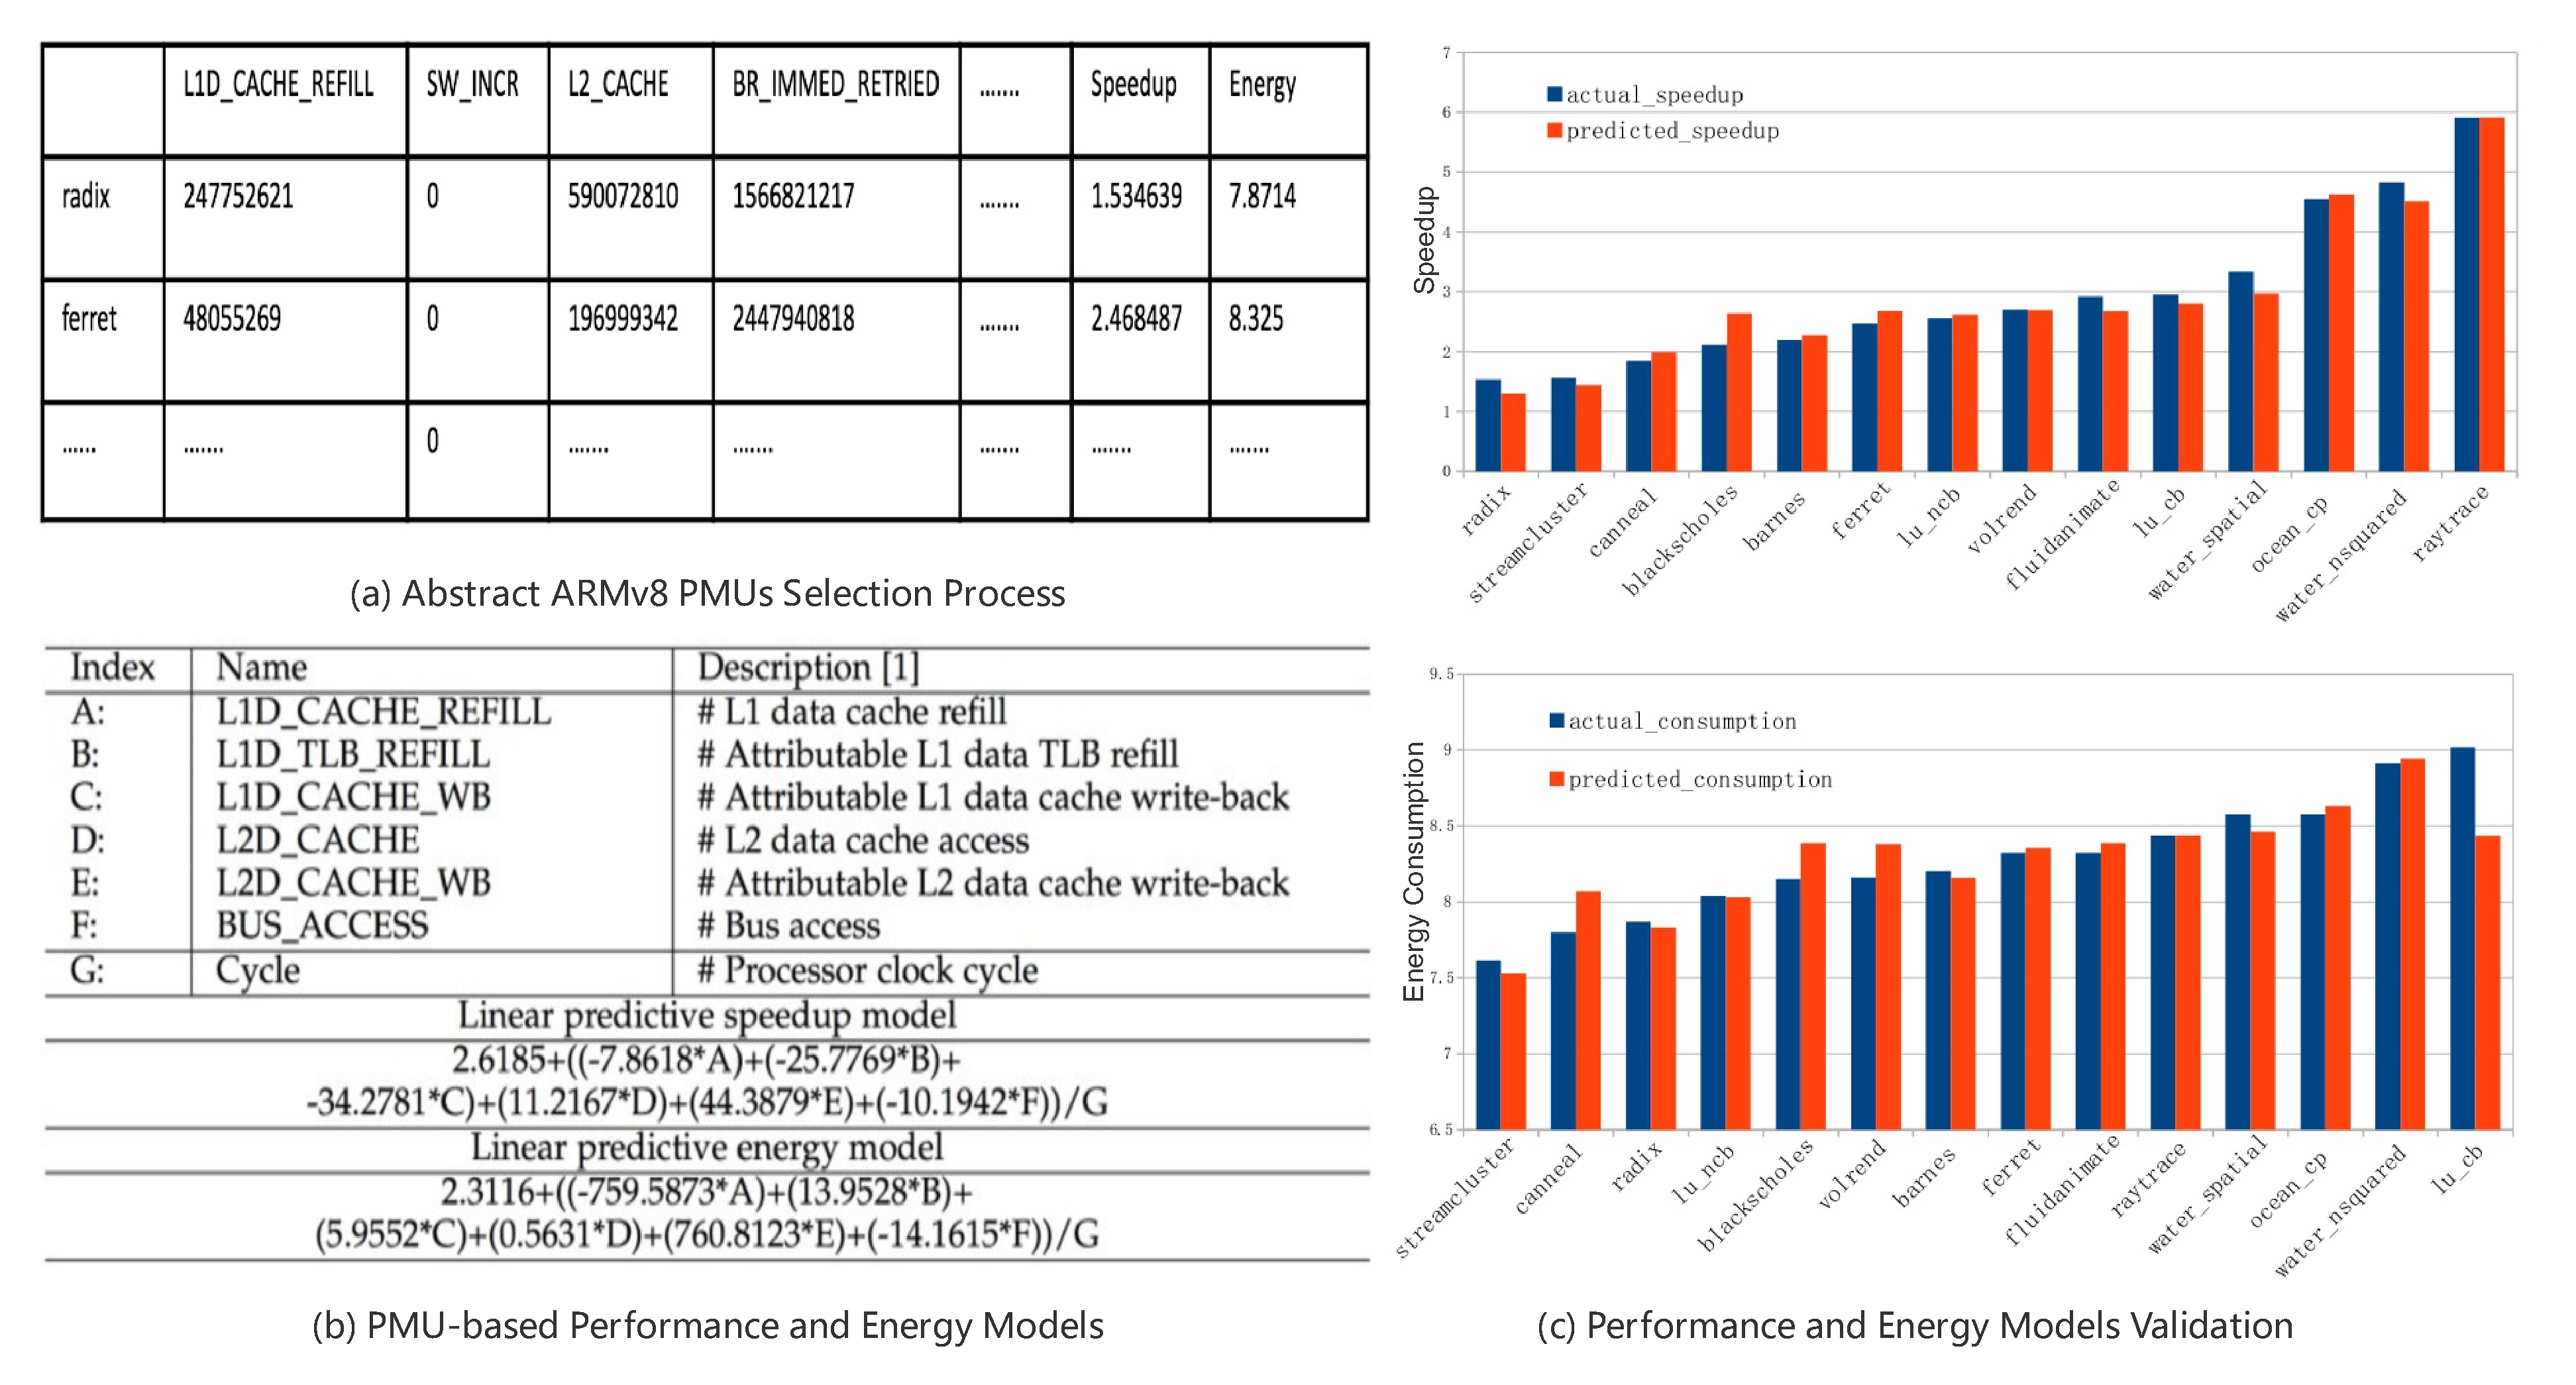
\includegraphics[scale=0.25]{figures/arm_model.pdf}
\caption{ARMv8 Performance and Energy Modelling}
\label{arm_model}
\end{figure*}

\ty{\section{Energy-Aware Scheduler Extension on ARMv8 Architecture}}

\ty{Furthermore, the energy consumption is a critical issue for multi-program co-execution on asymmetric multi-core processors. Different threads from application programs are variant between different type of cores. Followed by the prototype on GEM5 simulator, We fully-implement our COLAB scheduler on Linux kernel v3.16 with an energy-aware extension targeting ARMv8 architecture.} 

\begin{comment}
\begin{table}
  \caption{\ty{Selected ARMv8 PMUs and the Speedup and Energy Models}}
  \center
  \label{pca_arm_sp}
   \scalebox{0.8}{
   \begin{tabular}{p{0.8cm} | p{3.6cm} | p {5.4cm} c c c}
  \hline
     Index&  Name& Description \cite{ARMA57} \\
    \hline
     A: & L1D\_CACHE\_REFILL & \# L1 data cache refill\\
     B: & L1D\_TLB\_REFILL & \# Attributable L1 data TLB refill\\
     C: & L1D\_CACHE\_WB & \# Attributable L1 data cache write-back\\
     D: & L2D\_CACHE & \# L2 data cache access\\
     E: & L2D\_CACHE\_WB & \# Attributable L2 data cache write-back\\
     F: & BUS\_ACCESS & \# Bus access\\
     \hline
     G: & Cycle & \# Processor clock cycle\\
     \hline
     \multicolumn{3}{c}{Linear predictive speedup model}\\
     \hline
    \multicolumn{3}{c}{2.6185+((-7.8618*A)+(-25.7769*B)+}
    \\
    \multicolumn{3}{c}{-34.2781*C)+(11.2167*D)+(44.3879*E)+(-10.1942*F))/G}\\
 \hline
  \multicolumn{3}{c}{Linear predictive energy model}\\
     \hline
    \multicolumn{3}{c}{2.3116+((-759.5873*A)+(13.9528*B)+}
    \\
    \multicolumn{3}{c}{(5.9552*C)+(0.5631*D)+(760.8123*E)+(-14.1615*F))/G}\\
 \hline
  \end{tabular}}
\end{table}
\end{comment}

\ty{\subsection{Machine Learning based ARMv8 Performance and Energy Models}}

\ty{The abstract offline PMU selection process is shown in Fig.~\ref{arm_model}(a). We first run all benchmarks compiled in single-threaded version on either 4 Cortex-A73 or 4 Cortex-A53 configuration. We only record common PMUs used for both Cortex-A73 and Cortex-A53, together with each thread's relative speedup and energy consumption. We ignore the PMUs for which their value keep to be zero, such as \texttt{SW\_INCR} (Instruction architecturally executed, Condition code
check pass, software increment). For the remaining PMUs, we then apply the PCA technique to select the most important 6-PMU-combination. For example, it is easy to know that the performance and energy will be more dominated by the total data movement than some branch behaviours. As a result, although \texttt{BR\_IMMED\_RETIRED} is a meaningful PMU which counts all immediate branch instructions that are architecturally executed, but it is not selected after the PCA process as there are more important PMUs such as \texttt{L1D\_CACHE\_REFILL} (L1 data cache refill) and \texttt{L2\_CACHE} (L2 data cache access). }

\ty{The trained PMU-based ARMv8 performance and energy models are shown in Table~\ref{arm_model}(b).
In real ARM system validation, we use the clock cycle number to replace the GEM5 committed instructions as it is more stable recorded by a specialized register on the test board.}

\ty{We validate the accuracy of our trained models on each benchmark as shown in Fig.~\ref{arm_model}(c). The average error cross all benchmark for the performance model is around 7\% while for the energy model is around 1.5\%.}
%The range of these errors are within the normal performance and energy variance of the test board, so we can claim that the trained models are accuracy enough to predicate the system behaviours.}

\ty{\subsection{COLAB Algorithm Extension}}

\begin{algorithm}
\caption{Energy-aware COLAB extension}
\label{alg:2}
\begin{algorithmic}[]
\STATE \textbf{\_core\_alloctor\_e(thread\_struct\ $t$)}\{
\STATE \textbf{if} t.high\_hyper
\STATE \ \ \textbf{return} rr\_allocator\_(big\_cores)
\STATE \textbf{if} {t.low\_hyper \& t.low\_block}
\STATE \ \ \textbf{return} rr\_allocator\_(little\_cores)
\STATE \textbf{else return} rr\_allocator\_(cores) \}
\end{algorithmic}
\end{algorithm}

\ty{The original COLAB scheduler is extended to involve further collaboration to achieve energy-aware extension. Under this extension, a hyper-heuristic of a thread $t$ to guide core allocation is designed as follows:}
\ty{$$ hyper\_(t) = w_{s}*speedup(t) + w_{e}*energy(t) $$}
\ty{Where $w_{s}$ and $w_{e}$ are the trained weights of the speedup factor and energy consumption factor, separately; $energy(t)$ is the energy efficient factor for the thread $t$ between big and little cores. Energy efficient is the ratio of useful work done to the amount of power used as introduced in~\cite{tsirogiannis2010analyzing}. Similar with using linear regression on training PMUs for predicated speedup and energy consumption, this hyper-heuristic is trained by hierarchical regression to obtain the best trade-off between performance gain and energy saving.}

\ty{The extended energy-efficient core allocator \texttt{rr\_allocator\_e()} for the COLAB scheduling algorithm is presented in Alg.~\ref{alg:2}. Compared with the original version, it uses this hyper-heuristic to replace the speedup-heuristic in \texttt{rr\_allocator\_()}. Similar with mapping high speedup threads on big cores, this trade-off allocation policy is applied to avoid heavy energy consumption on big cores. When the energy-aware extension is enabled, threads labeled by this hyper-heuristic involve both the performance and energy concerns instead of the predicated speedup only. Under this hyper-heuristic, core allocator can provide the energy-aware solutions. It only allocates high speedup and non-energy-intensive threads to big cores, while keeps energy-intensive threads on little cores even they also have some kind of speedup.} 

\ty{\subsection{Scheduling Overhead Analysis}}
The overhead of the performance model is small. It is updated only every 10 msec and it requires the evaluation of the linear regression equation for each thread. 

\ty{To maintain per task runtime counter information, we need to access the hardware PMUs every time we context switch. By using register to read a PMU directly, it takes 4 cycles on the Cortex-A53 and 14 cycles on the Cortex-A73. We need to read 7 PMUs in sequential each time.}

The rest of scheduling overhead comes from labeling all threads based on predicted speedup and blocking level every 10 msec. This is similar to the scheduling overhead of WASH and is infrequent enough to not affect us.


\section{Experimental Evaluation}

\subsection{Experimental Setup}

% \begin{table}[htbp]
%  \caption{Benchmarks categorization~\cite{bienia08characterization,woo1995splash,southern2016analysis}}
%  \center
%  \label{BC}
%   \scalebox{1}{
%   \begin{tabular}{ p{2.1cm} |  p{1.6cm} | p{1.6cm} | p{1.4cm} }
%     \hline
%    Name & Sync. Rate & Comm/Comp Ratio & No. Threads\\
%    \hline
%    blackscholes &  low & high & 1 + n \\
%    bodytrack &  medium & high & 2 + n\\
%    dedup &  medium & high & 3 + 3n\\
%    ferret &  high & medium & 3 + 4n\\
%    fluidanimate &  very high & low & 1 + n\\
%    freqmine &  high & high & n\\
%    swaptions &  low & low & 1 + n\\
%    radix &  low & high & n\\
%    lu\_ncb & low & low & n \\
%    lu\_cb &  low & low & n\\
%    ocean\_cp &  low & low & n\\
%    water\_nsquared &  medium & medium & n\\
%    water\_spatial &  low & low & n\\
%    fmm &  medium & low & n\\
%    fft &  low & high & n\\
%    \hline
%    % \bottomrule
%  \end{tabular}}
%\end{table}

% VJ: OLD VERSION
%\textbf{\textit{Experimental Environment:}} We ran our experiments on GEM5, simulating an ARM big.LITTLE-like architecture. The big cores are similar to out-of-order 2 GHz CortexA57 cores, with a 48 KB L1 instruction cache, a 32 KB L1 data cache, and a 2 MB L2 cache. The little cores are similar to in-order 1.2 GHz CortexA53 ones, with a 32 KB L1 instruction cache, a 32 KB L1 data cache, and a 512 KB L2 cache. We evaluated four distinct hardware configurations: 2B2S,2B4S,4B2S,4B4S, where B denotes big cores and S denoted little cores.
%%Two had balanced numbers of big and little cores, one with two big and two little cores (2B2S) and one with four big and four little ones (4B4S). The other two had different numbers of big and little cores, one with two big and four little cores (2B4S) and one with four big cores and two little cores (4B2S). 
%The OS is Linux v3.16. We cross-compiled the kernel with gcc v5.4.0, while we compiled the benchmarks inside the emulated environment with gcc v4.8.2.
%We chose to use a simulated environment to make it easier to evaluate our approach on multiple different hardware configurations. While we targeted simulated ARM cores, the underlying general procedure and model can be implemented on any real processor as long as they provide enough hardware performance monitor units (PMU). All hardware counters used by our model are supported by the real ARM Cortex-A57/A53 \cite{ARMA57} PMU.

\textbf{\textit{Experimental Environment:}} We first ran our experiments on GEM5, simulating an ARM big.LITTLE-like architecture. The big cores are similar to out-of-order 2 GHz CortexA57 cores, with a 48 KB L1 instruction cache, 32 KB L1 data cache and 2 MB L2 cache. The little cores are similar to in-order 1.2 GHz CortexA53 ones, with a 32 KB L1 instruction cache, 32 KB L1 data cache and 512 KB L2 cache. We evaluated four distinct hardware configurations on GEM5: 2B2S, 2B4S, 4B2S, 4B4S, where B denotes big cores and S denoted little cores.
%%Two had balanced numbers of big and little cores, one with two big and two little cores (2B2S) and one with four big and four little ones (4B4S). The other two had different numbers of big and little cores, one with two big and four little cores (2B4S) and one with four big cores and two little cores (4B2S). 
% VJ : I would get rid of the OS and compiler version...Unless it matters which kernel we are using
%The OS is Linux v3.16. We cross-compiled the kernel with gcc v5.4.0, while we compiled the benchmarks inside the emulated environment with gcc v4.8.2.
%We chose to use a simulated environment to make it easier to evaluate our approach on multiple different hardware configurations.
%While we targeted simulated ARM cores, the underlying general procedure and model can be implemented on any real processor as long as they provide enough hardware performance monitor units (PMU). All hardware counters used by our model are supported by the real ARM Cortex-A57/A53 \cite{ARMA57} PMU.
We then validate COLAB and its energy-aware extension on a HiHope Hikey 970 development board with 4 Cortex-A73 big cores at 2.36GHz and 4 Cortex-A53 little cores at 1.8GHz. As there is only 4 big cores in total to produce baseline performance, we evaluate four configurations: 1B1S, 1B3S, 2B2S and 3B1S. 

 \begin{table}[htbp]
  \caption{Benchmarks categorization~\cite{bienia08characterization,woo1995splash,southern2016analysis}}
  \center
  \label{BC}
   \scalebox{1}{
   \begin{tabular}{ p{2.5cm} |  p{2.0cm} | p{3cm} }
     \hline
     Name & Sync. Rate & Comm/Comp Ratio\\
    \hline
    blackscholes &  low & high \\
    bodytrack &  medium & high \\
    dedup &  medium & high \\
    ferret &  high & medium \\
    fluidanimate &  very high & low \\
    freqmine &  high & high \\
    swaptions &  low & low \\
    radix &  low & high \\
    lu\_ncb & low & low \\
    lu\_cb &  low & low \\
    ocean\_cp &  low & low \\
    water\_nsquared &  medium & medium \\
    water\_spatial &  low & low \\
    fmm &  medium & low \\
    fft &  low & high \\
    \hline
    % \bottomrule
  \end{tabular}}
\end{table}


 \begin{table*}
  \caption{Multi-programmed Workloads Compositions}
  \center
  \label{WC}
   \scalebox{0.9}{
   \begin{tabular}{ p{2cm} | p{7cm} | p{4cm} | p{2cm} }
    \hline
     \multicolumn{4}{c}{Synchronization-intensive VS Non-synchronization-intensive Workloads}\\
    \hline
     Index & Workload Composition & Synchronizations & Threads \\
    \hline
    Sync - 1 & water\_nsquared - fmm & intensive & 4 \\
    Sync - 2 & dedup - fluidanimate & intensive & 18 \\
    Sync - 3 & water\_nsquared - fmm - fluidanimate - bodytrack & intensive & 9 \\
    Sync - 4 & dedup - ferret - fmm - water\_nsquared & intensive & 20\\
    \hline
    NSync - 1 & water\_spatial - lu\_cb & non-intensive & 4 \\
    NSync - 2 & blackscholes - swaptions & non-intensive & 16 \\
    NSync - 3 & radix - fft - water\_spatial - lu\_cb & non-intensive & 8\\
    NSync - 4 & blackscholes - ocean\_cp - lu\_ncb - swaptions & non-intensive & 20\\
     \hline
     \multicolumn{4}{c}{Communication-intensive VS Computation-intensive Workloads}\\
     \hline
     Index & Workload Composition & Comm/Comp & Threads \\
    \hline
    Comm - 1 & water\_nsquared - blackscholes & Communication-intensive & 4 \\
    Comm - 2 & ferret - dedup &  Communication-intensive & 16 \\
    Comm - 3 & water\_nsquared - fft - radix - bodytrack &  Communication-intensive & 9 \\
    Comm - 4 & blackscholes - dedup - ferret - water\_nsquared &  Communication-intensive & 20\\
    \hline
    Comp - 1 & water\_spatial - fmm & Computation-intensive & 4 \\
    Comp - 2 & fluidanimate - swaptions & Computation-intensive & 17 \\
    Comp - 3 & lu\_ncb - fmm - water\_spatial - lu\_cb & Computation-intensive & 8\\
    Comp - 4 & fluidanimate - ocean\_cp - lu\_ncb - swaptions & Computation-intensive & 20\\
    \hline
      \end{tabular}}
  \scalebox{0.8}{
  \begin{tabular}{p{1.5cm} |p{4cm} |p{1cm}|| p{1.5cm} |p{7cm} |p{1cm}}
    \multicolumn{6}{c}{Large Mixed Multi-programmed Workloads for Real System Validation}\\
    \hline
   Index & Workload Composition & Threads & Index & Workload Composition & Threads\\
    \hline
    Large - 1 & radix - ocean\_cp & 5 & Large - 3 & blackscholes - radix - fluidanimate - water\_spatial & 15\\
    Large - 2 & ferret - swaptions & 24 & Large - 4 & ocean\_cp - ferret - lu\_cb - swaptions & 29\\
    \hline
  \end{tabular}}
\end{table*}

\begin{comment}
  \scalebox{0.8}{
  \begin{tabular}{p{1.5cm} |p{4cm} |p{1cm}|| p{1.5cm} |p{7cm} |p{1cm}}
   \hline 
  \multicolumn{6}{c}{Random-mixed Multi-programmed Workloads}\\
  \hline
      Index & Workload Composition & Threads & Index & Workload Composition & Threads\\
   \hline
    Rand - 1 &lu\_cb - dedup & 19& Rand - 6 &water\_spatial - fmm - fft - fluidanimate &21\\
    Rand - 2 &lu\_ncb - bodytrack &10& Rand - 7 &fmm - water\_spatial - ferret - swaptions&20\\
    Rand - 3 &ferret - water\_spatial&9 & Rand - 8 &water\_spatial - water\_nsquared - ferret - freqmine&17\\
    Rand - 4 &ocean\_cp - fft&8 & Rand - 9 &blackscholes - bodytrack - dedup - fluidanimate&55\\
    Rand - 5 &freqmine - water\_nsquared&6 & Rand - 10 &lu\_cb - lu\_ncb - bodytrack - dedup&53\\
   \hline
  \end{tabular}}
%\end{table*}
\end{comment}

\textbf{\textit{Workloads:}} For our workloads we used 15 different benchmarks (Table~\ref{BC}), pulled from PARSEC3.0~\cite{bienia11benchmarking} and SPLASH2~\cite{woo1995splash}.
%\footnote{Our version of GEM5 cannot simulate all PARSEC3.0 benchmarks on ARM. On top of \emph{canneal} and \emph{raytrace} that other researchers have also failed to build~\cite{endo2014micro,van2013full}. Among the SPLASH2 benchmarks, \emph{cholesky} and \emph{volrend} depended on huge input data files that did not fit on the hard drive image. We could not use \emph{barnes}, \emph{radiosity}, \emph{facesim}, \emph{x264}, \emph{vips} and \emph{streamcluster} because their runtime is prohibitively long even for $simsmall$ inputs.}
We only use the \emph{simsmall} inputs on GEM5 as it is well-known that the simulation is extremely slow. We group the benchmarks based on two criteria: a) synchronization intensity and b) communication vs computation intensity.
For each group, we randomly generate workloads with variable numbers of benchmarks and threads. These workloads allow us to investigate the behavior of the three scheduling policies under different extremes.
We then use large mixed workloads with the \emph{simlarge} inputs on  HiHope  Hikey  970 to explore the general  cases and validate COLAB with its energy-aware extension on the real chip with asymmetric multi-core processors.
Table~\ref{WC} shows the selected workloads. 

%For all of them, the experiment starts from a checkpoint taken after all benchmarks have completed their initialization.

%Each individual result represents the average over two simulations with different core orders - either big cores first or little cores first. Even small variations in the initial state of the system can have a significant effect on scheduling decisions and thus performance. For the Linux scheduler in particular, the order of starting benchmarks will decide which benchmarks will be initially assigned to big and little cores. By varying the initial state and measuring average runtimes over multiple simulations, we minimize the effect of randomness on our evaluation.

\textbf{\textit{Performance Metrics:}} Our evaluation uses two metrics to quantify scheduling efficiency: {\it Heterogeneous Average Normalized Turnaround Time} (H\_ANTT) and {\it Heterogeneous System Throughput} (H\_STP). They are based on ANTT and STP, as introduced in~\cite{eyerman2008system}. Both ANTT and STP use as their baseline the runtime of each application when executed on its own, i.e. when there is no resource sharing and scheduling decisions have little effect. ANTT is the average slowdown of all applications in the mix relative to their isolated baseline runtime. STP is the sum of the throughputs of all applications, relative to their isolated throughput.

For AMPs, these two metrics fail to work as intended. The runtime when executed alone is still affected by scheduling decisions, e.g. which threads to run on big cores. To overcome the problem, our modified metrics H\_ANTT and H\_STP use the runtime of each application in the mix when executed alone \emph{on a system where there are only big cores}. If the turnaround time of each application $i$ while being co-scheduled is $T^{M}_i$ and the turnaround time for the same application when running alone on a big-only system is $T^{SB}_i$, then:
$$ H\_ANTT = \frac{1}{n}\sum^{n}_{i=1}\frac{T^{M}_i}{T^{SB}_i}
,\ \ H\_STP = \sum^{n}_{i=1}\frac{T^{SB}_i}{T^{M}_i}$$
%When we evaluate a single benchmark on its own, we use the {\it Heterogeneous Normalized Turnaround Time} (H\_NTT):
%$$ H\_NTT = \frac{T^{M}}{T^{SB}}$$
H\_ANTT is better when lower, H\_STP is better when higher. For most figures, we further normalize our results relative to the Linux CFS results for the same configuration and workload.

\textbf{\textit{Schedulers:}}
We evaluate COLAB by comparing it against the default Linux CFS scheduler~\cite{molnar2007cfs} and a state-of-the-art realistic scheduler based on WASH~\cite{jibaja2016portable}. 
Linux CFS is the default scheduler on the GEM5 simulator and ARM GTS~\cite{jeff2013big} is the default scheduler on the development board. They provide fairness while trying to maximize the overall CPU resource utilization.
%The original WASH was implemented inside a Java VM to control Java thread affinities.
%In our re-implementation of WASH, we use the same heuristic but we drive it with a core sensitivity model that fits the simulated system and we use it for controlling all application threads. 

%\begin{figure}
%\centering
%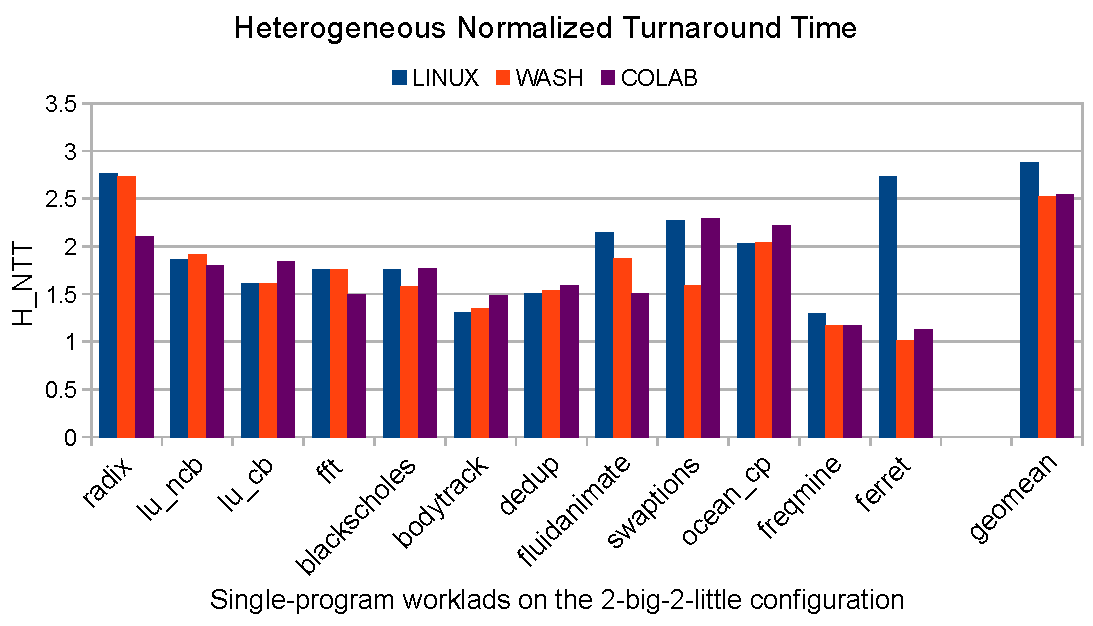
\includegraphics[scale=0.48]{figures/MSW2.pdf}
%\caption{Performance of single program workloads on a 2-big 2-little system. Lower is better.}
%\label{MSW}
%\end{figure}  

%\subsection{Single-programmed Workloads}
%Much of the research on AMP scheduling focuses on single-programmed workloads, where fairness and load balancing are not important and the focus is on core sensitivity and bottleneck acceleration. In this section, we examine how COLAB fares under this scenario. Figure~\ref{MSW} shows H\_NTT under Linux (blue), WASH (red) and COLAB (violet), for our multi-threaded benchmarks when executed alone on a 2-big-2-little hardware configuration. 
%We do not consider the three SPLASH2 benchmarks \emph{fmm}, \emph{water\_nsquared} and \emph{water\_spatial}, since they do not support more than 2 threads with $simsmall$ input size on GEM5 and scheduling them optimally for performance is trivial.

%The AMP-agnostic Linux scheduler is inappropriate for most benchmarks. COLAB improves H\_NTT by up to 58\% and by 12\% on average and up to 173\% over Linux CFS for \emph{ferret}, where most computation happens in a pipeline pattern with unbalanced stages. AMP-aware schedulers take advantage of that by scheduling the longest stages, the bottleneck threads, on big cores. As a result, COLAB does only 13\% worse than running on a system \emph{with four big cores}.
%Compared to WASH, COLAB achieves its best result for \emph{fluidanimate}. Previous work~\cite{bienia08characterization} has shown that \emph{fluidanimate} has around 100x more lock-based synchronizations than other PARSEC applications. Our collaborative core allocation and thread selection policy is much better than WASH at prioritizing bottleneck threads.  As a result, we reduce turnaround time by 30\% compared to Linux and 20\% compared to WASH.
%In some cases, such as \emph{bodytrack}, \emph{lu\_ncb}, or \emph{freqmine}, AMP-awareness has little effect on performance. Such benchmarks split work dynamically between threads, which then all have the same core sensitivity and the application adapts automatically to asymmetries in processing speed. AMP-aware policies offer no benefit while introducing overheads, as was also noted in~\cite{jibaja2016portable}. The pipeline benchmark \emph{dedup} has five stages to stream the input set. When there are more threads than available cores, both heterogeneous-aware schedulers can not service the excess threads in time, resulting in a certain impact on overall system performance.
%There is only one case where COLAB performs significantly worse than WASH. For \emph{swaptions}, we perform as well as the AMP-agnostic Linux scheduler while WASH improves turnaround time by 31\%. This is because the bottleneck threads of \emph{swaptions} are core insensitive while the non-bottleneck threads are core sensitive. This being the ideal case for WASH, it improves turnaround time while we fail to do the same.

%On average, WASH and COLAB perform similarly well and improve performance by 12\% compared to Linux when handling single program workloads. This is a limited scenario, with no need for fairness and a simple decision space. COLAB was not expected to perform much better than the state-of-the-art, doing as well as it is a positive result.
%\vspace{-1.2em}
\subsection{Experiments on GEM5}
%\vspace{-0.3cm}
In this section, we evaluate the performance of the COLAB scheduler for multi-threaded multi-program workloads using the GEM5 simulator. We demonstrate that COLAB outperforms both the Linux CFS and WASH when there is room for improvement. In particular, where there is a limited number of big cores and/or where the workload contains communication-intensive benchmarks, it is beneficial to consider core affinity and thread bottlenecks \emph{at the same time}. In this setting, the advantages of COLAB over Linux CFS and WASH become apparant. In the rest of this subsection, we examine in more detail the behavior of COLAB under four different hardware configurations
(2B2S, 2B4S, 4B2S, 4B4S) 
for the five different classes of workloads shown in Table~\ref{WC}.

\begin{figure}
\centering
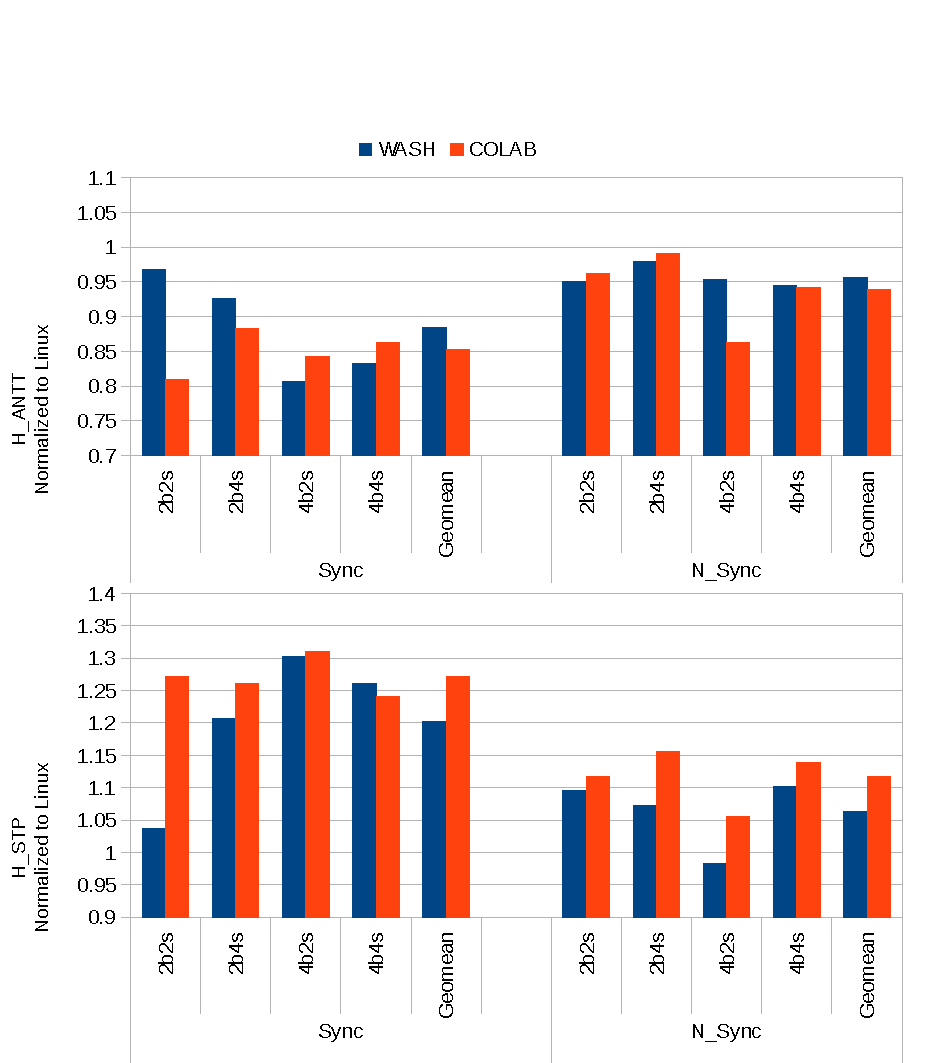
\includegraphics[scale=0.55]{figures/sync.pdf}
%\caption{Heterogeneous Average Normalized Turnaround Time (H\_ANTT) and Heterogeneous System Throughput (H\_STP) 
\caption{Performance of Synchronization-Intensive and Non-Synchronization-Intensive Workloads. All results are normalized to the Linux CFS ones. Lower is better for H\_ANTT and higher is better for H\_STP.}
\label{sync}
\end{figure} 

\textbf{\textit{Synchronization-intensive vs Synchronization Non-intensive workloads:}}
The \emph{synchronization-intensive} workloads comprise benchmarks with high synchronization rates, having a large number of bottleneck threads. We expect that COLAB should be able to schedule them better than CFS and WASH. Conversely, \emph{synchronization non-intensive} workloads should provide fewer opportunities for COLAB to improve on CFS and WASH.

Figure~\ref{sync} shows the performance of all three schedulers for each workload class and hardware configuration. The two plots show the 
average H\_ANTT (top) and the average H\_STP (bottom). In each plot, we show the results for both the synchronization-intensive (\emph{Sync}, left half) and synchronization non-intensive (\emph{N\_Sync}, right half) classes of workloads.
The results confirm our expectations. We can observe that COLAB improves the turnaround time of \emph{Sync} workloads by around 15\% and 4\% on average compared to CFS and WASH, respectively. We can also see that hardware configurations with low core counts (e.g.~2B2S) favor COLAB, allowing it to reduce turnaround time by up to 20\% compared to CFS and by up to 16\% compared to WASH. With fewer cores, run queues of cores become longer, requiring careful balancing between bottleneck acceleration and core sensitivity. WASH places all bottleneck threads onto the big cores, making these cores congested and ending up with only 3\% performance improvement over CFS. COLAB handles these bottleneck threads in a more holistic way, improving turnaround time by 20\% and system throughput by 27\%, compared to CFS.
%
On the other hand, the \emph{N\_Sync} workloads contain fewer bottleneck threads, making scheduling decisions much easier. As a result of this, both COLAB and WASH perform similarly to CFS, with COLAB improving average turnaround time by 6\% and average system throughput by 12\% compared to CFS.
An interesting point is that COLAB significantly outperforms (by 10\% and 15\% in turnaround time) WASH and Linux for \emph{N\_Sync} workloads on the 4B2S configuration. In this case, there is not enough critical threads to utilize big cores and WASH keeps needlessly migrating predicted critical threads between big cores. COLAB, on the other hand, makes intelligent decisions by keeping more threads on little cores, giving more more chance to big cores to execute the few \emph{really critical} threads as soon as possible.
% (PP: Turnaround time is worse for COLAB. Unless we go into details about why turnaround time is worse while throughput is better, saying that we do slightly better is wrong. Also it would be nice for the previous paragraph to identify the specific workloads which are accelerated more and pinpoint what makes COLAB better in this case.) 
%This also explains why WASH does slightly better than COLAB on 2B4S configuration for these workloads - When there are not enough critical threads to be accelerated, the low big-to-little ratio could guide the WASH to migrate less threads on big cores while COLAB does not sensitive to this ratio. 

\begin{figure}
\centering
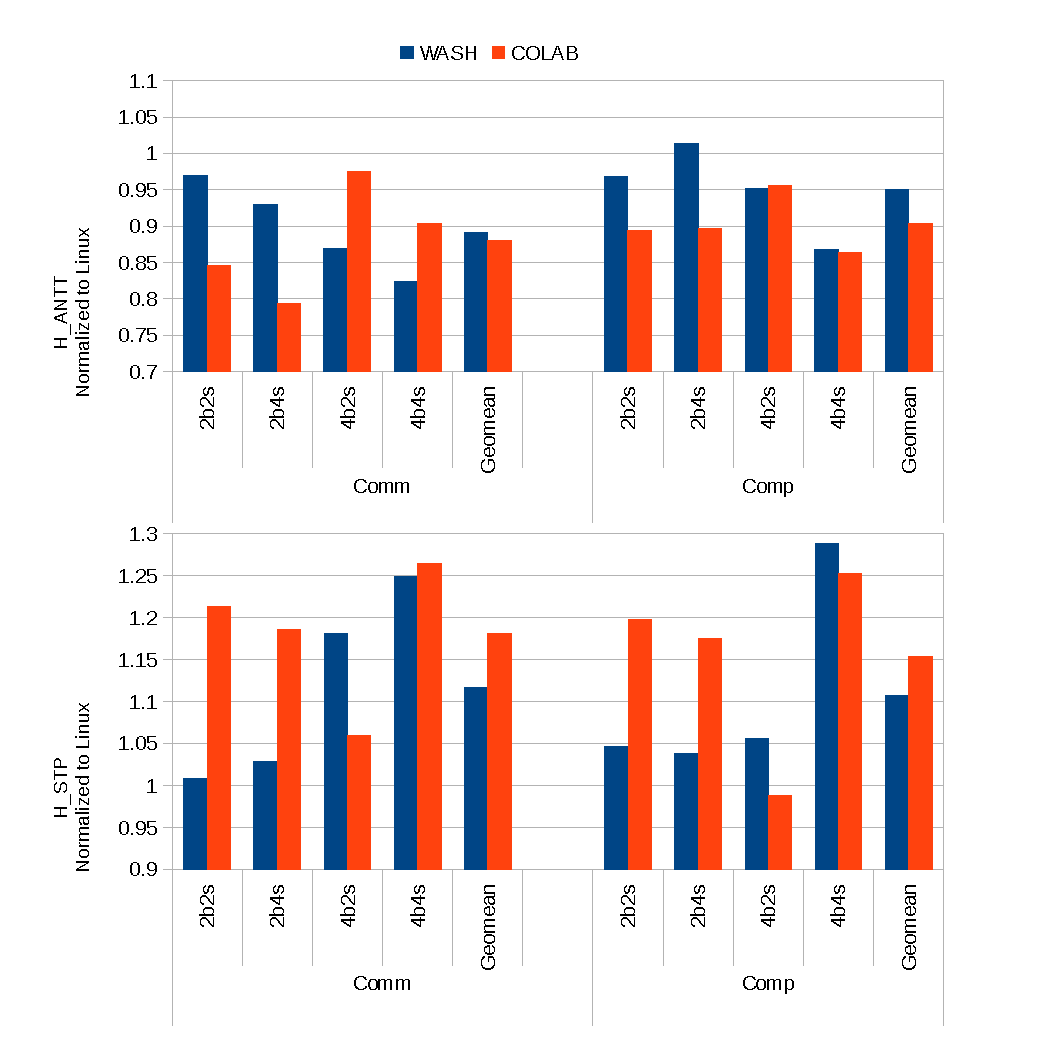
\includegraphics[scale=0.55]{figures/com.pdf}
%\caption{Heterogeneous Average Normalized Turnaround Time (H\_ANTT) and Heterogeneous System Throughput (H\_STP)
\vspace{-0.35cm}
\caption{Performance of Communication-Intensive and Computation-Intensive Workloads. All results are normalized to the Linux CFS ones. Lower is better for H\_ANTT and higher is better for H\_STP.}
\label{com}
\end{figure} 

% VJ: Got to here
\textbf{\textit{Communication-intensive vs Computation-intensive workloads:}}
When handling programs with high communication-to-computation ratios, bottleneck threads are likely to arise and accelerating them is critical. This is an ideal scenario for COLAB. On the other hand, workloads with little communication are easier to schedule, so CFS and WASH should do reasonably well, leaving little space for improvement.

Figure~\ref{com} shows the evaluation results for these two classes of workloads, \emph{Comm} and \emph{Comp}. Both COLAB and WASH improve over the Linux scheduler for communication-intensive workloads. They, however, offer different advantages on different hardware configurations. COLAB distributes the bottleneck threads to both big and little cores which is extremely important when having only two big cores (2B2S, 2B4S). COLAB improves the turnaround time by up to 21\% compared to Linux and 15\% compared to WASH on the 2B4S configuration. When more big cores are available, WASH does better as it keeps all bottleneck threads on big cores. On these configurations, WASH improves turnaround time by up to 18\% over Linux (on the 4B4S configuration) and up to 10\% over COLAB (on the 4B2S configuration). On average, COLAB reduces turnaround time by around 12\% compared to Linux and 1\% compared to WASH for the communication-intensive workload class.
Figure~\ref{com} also confirms that there are few opportunities for better scheduling with computation-intensive workloads. Still, COLAB does better than WASH and Linux. Its turnaround time and system throughput are improved by around 10\% and 15\%, respectively, compared to Linux and 5\% compared to WASH. This is, again, due to a fact that multiple bottlenecks are distributed both to big and little cores, which results in more efficient use of the available hardware resources for the few bottlenecks that are present.

\begin{comment}
\begin{figure}
\centering
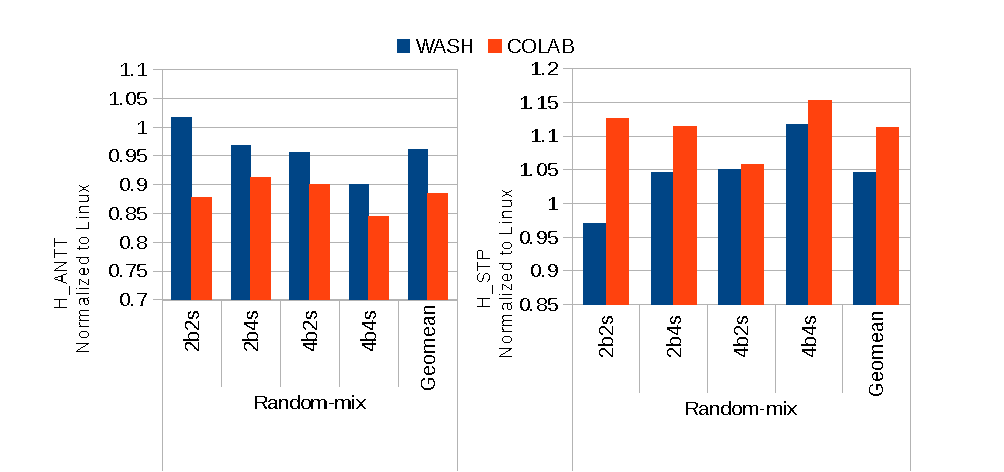
\includegraphics[scale=0.55]{figures/rand.pdf}
%\caption{Heterogeneous Average Normalized Turnaround Time (H\_ANTT) and Heterogeneous System Throughput (H\_STP)
\caption{Performance of 2- and 4-programmed Workloads. All results are normalized to the Linux CFS ones. Lower is better for H\_ANTT and higher is better for H\_STP.}
\label{rand}
\vspace{-0.2cm}
\end{figure} 
%\vspace{-1em}
\textbf{\textit{Mixed workloads:}}
This class of workloads represents the general case of different applications with different needs, affinities, and communication patterns competing for the same cores. Figure~\ref{rand} shows the results for 10 such workloads. COLAB performs very well for these workloads: more diverse programs mean more asymmetry, more bottlenecks, more critical threads, and more potential for acceleration. Our collaborative multi-factor scheduler carefully balancing all scheduling aims (core sensitivity, thread criticality and fairness) leads to a significant performance gain against WASH and Linux. COLAB improves turnaround time and system throughput by around 12\% and 11\% compared to Linux and around 8\% and 7\% compared to WASH.
\end{comment}
%\vspace{-1em}
\begin{figure}
\centering
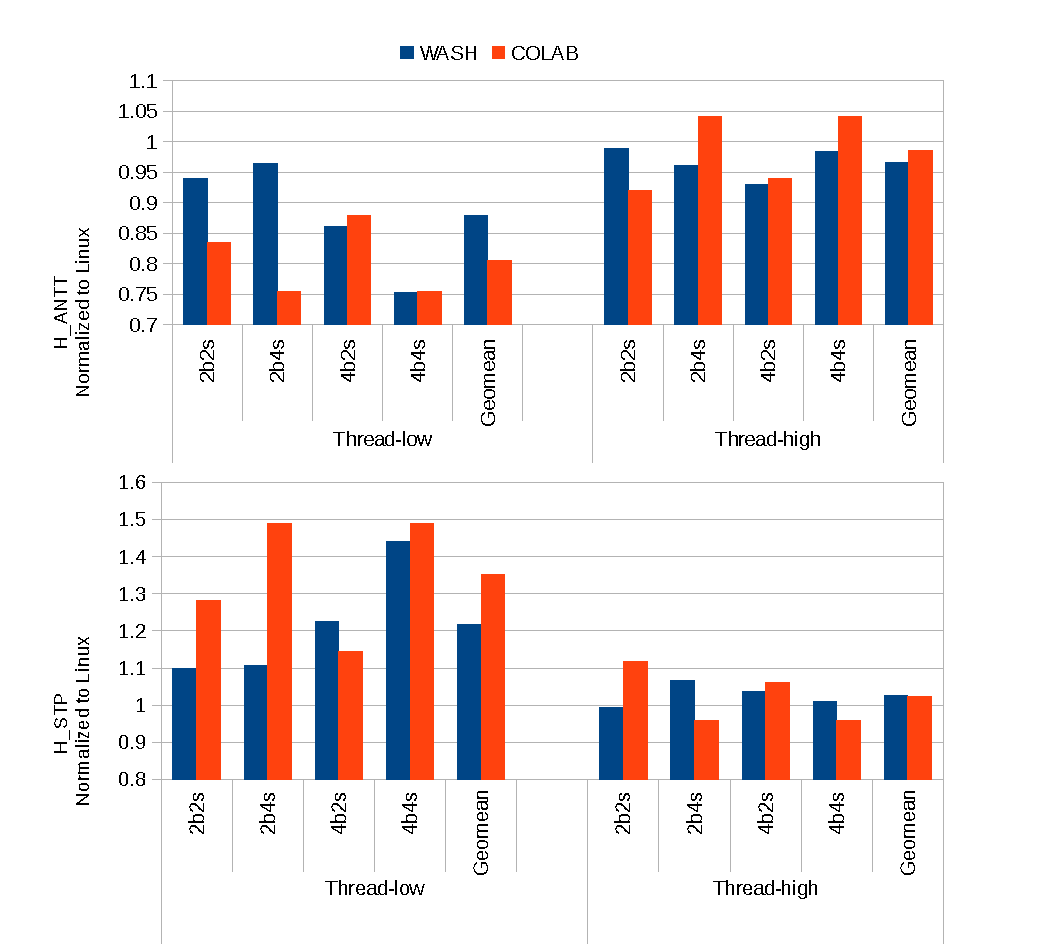
\includegraphics[scale=0.55]{figures/nthread.pdf}
%\caption{Heterogeneous Average Normalized Turnaround Time (H\_ANTT) and Heterogeneous System Throughput (H\_STP) 
\caption{Performance of low number of application threads and high number of application threads Workloads. All results are normalized to the Linux CFS ones. Lower is better for H\_ANTT and higher is better for H\_STP.}
\label{nthread}
\end{figure}
%\vspace{-1em}

\begin{figure}
\centering
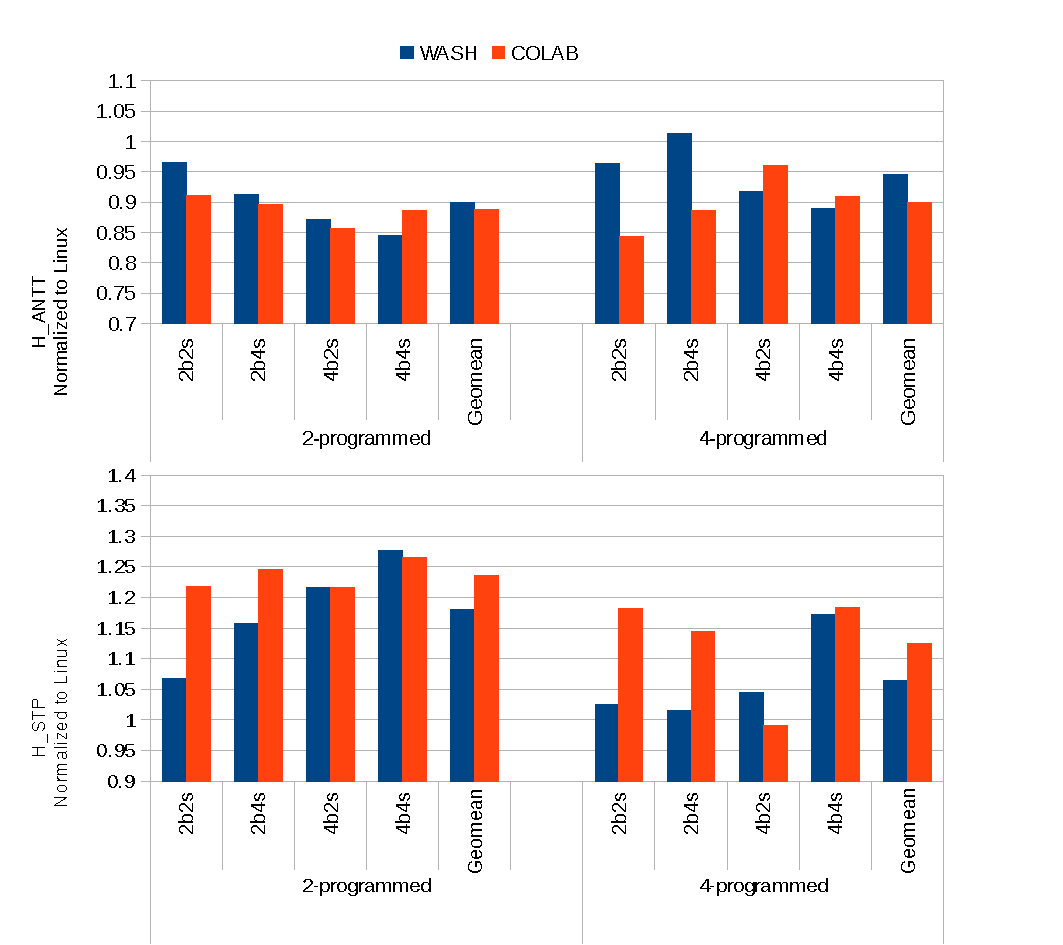
\includegraphics[scale=0.55]{figures/nprog.pdf}
%\caption{Heterogeneous Average Normalized Turnaround Time (H\_ANTT) and Heterogeneous System Throughput (H\_STP)
\caption{Performance of 2- and 4-programmed Workloads. All results are normalized to the Linux CFS ones. Lower is better for H\_ANTT and higher is better for H\_STP.}
\label{nprog}
\end{figure}
%\vspace{-1em}
%\begin{figure*}
%\centering
%\includegraphics[scale=0.6]{figures/all.png}
%\caption{Heterogeneous Average Normalized Turnaround Time (H\_ANTT) and Heterogeneous System Throughput (H\_STP)of multiprogrammed workloads averaged by different configurations. All results are normalized to the Linux CFS ones.}
%\label{M24W}
%\end{figure*}
\textbf{\textit{Thread and program count:}}
To examine the impact of thread and program count on the behavior of each scheduler, we grouped our experimental results based on these two properties. Figure~\ref{nthread} shows the performance of all schedulers both for workloads with a low thread count (less than the core count for that hardware configuration) and for workloads with a high thread count (at least double higher than the maximum core count). We observe that both COLAB and WASH perform significantly better than Linux for workloads with a low number of threads. Fewer threads make it easier to identify bottleneck threads and give them the resources they need - either by migrating them to big cores (WASH and COLAB) or by prioritizing them on little cores (COLAB). With limited big core resources, COLAB does much better than WASH since it distributes bottleneck threads on all available cores, avoiding overloading the few big cores and keeping the little cores idle. COLAB outperforms Linux by up to 25\% (2B4S) and WASH by up to 21\% (2B4S) on turnaround time. On average, COLAB improves turnaround time and system throughput by around 20\% and 35\% compared to Linux and around 8\% and 11\% compared to WASH for workloads with a low number of threads.
For workloads with a high thread count, neither Linux nor WASH are able to improve much on Linux. Overloading the system with threads means that, regardless of where we place threads, cores will have long runqueues. 
In this case, all cores will have long run queues and COLAB and WASH increase the management overhead (including more frequent thread migrations) with little benefit, leading to performance degradation. Of the two heterogeneity-aware schedulers, COLAB, with its scale-slice technique, more frequently migrates threads, which results in a slightly worse performance than WASH. On average, COLAB improves turnaround time and system throughput by less than 2\% and 3\% compared to Linux, while WASH slightly outperforms COLAB by 2\% on turnaround time and 0.2\% on system throughput.

We see a similar picture when we considered workloads with different number of programs in them. Figure~\ref{nprog} shows the performance of all schedulers for 2-programmed and 4-programmed workloads. As in the case of high and low thread counts, increasing the number of co-executed programs gives higher pressure on the scheduler, increasing the waiting time of threads in runqueues and reducing the direct benefit of migration between waiting threads. But more programs also cause more bottlenecks and provide new opportunities for co-acceleration instead of only increasing data-parallel threads. 
%. Heterogeneous aware schedulers generally enjoy better performance gain against Linux on workloads with less programs. Similar as the issue in the above comparisons for total number of threads, more programs with more threads increase the waiting list on runqueues and reduce the direct benefit of migrations between waiting programs/threads.
By intelligently distributing bottleneck threads from different programs between big and little cores, COLAB faces less problems than WASH from the pressure of increasing programs. 

As a result, both COLAB and WASH outperform Linux by more than 10\% on 2-programmed workloads on turnaround time and COLAB can keep the 10\% performance gain also on 4-programmed workloads, while WASH reduced to only have 5\% performance gain on 4-programmed workloads. As for system throughput, COLAB improves by 23\% and 12\% on 2-programmed and 4-programmed workloads compared to Linux while improves by 5\% and 6\% on 2-programmed and 4-programmed workloads compared to WASH. 
%\textbf{VJ: This is a bit counterintuitive. Why do we get better results for COLAB scheduler when we have more programs but not when we have more threads in a workload?}


%\begin{itemize}
%\item \textbf{Synchronisation-intensive} workloads comprise of the programs that have high synchronisation rate. Our hypothesis was that these workloads contain more bottleneck threads, due to intensive synchronisation between different threads, and that the mechanisms we developed in COLAB scheduler will schedule these threads in more optimal way, compared to Linux and WASH schedulers. On the other hand, \textbf{Synchronisation-Nonintensive} workloads comprise of the programs that have low synchronisation rate, hence giving less opportunities to the COLAB scheduler to improve on Linux and WASH schedulers. Therefore, for these workloads we expected to see less impact from COLAB.
%\item \textbf{Communication-intensive} workload comprise of the programs that have high communication-to-computation ratio. This result in high volume of communication between program threads, which furher results not only in more bottleneck threads, but also in low amount of computation done by some threads. This scenario gives more opportunities to COLAB for improved scheduling decisions, therefore our hypothesis was that for these workloads we will get better results than Linux and WASH. \textbf{Computation-intensive} workloads comprise of applications that have high computation-to-communication ratio. Due to less bottleneck threads and more similarity in terms of computation load of each thread, there are less opportunities for the COLAB scheduler here to improve on Linux and WASH, therefore we expected similar results between all three scheduler.
%\item \textbf{Mixed} workloads represent the most general workloads, comprising a mixture of synchronisation-intensive, synchronisation-nonintensive, communication-intensive and computation-intensive programs. The intention of using these workload is to observe how well COLAB performs in general setting, compared to Linux and WASH.
%\end{itemize}

%\begin{figure}
%\centering
%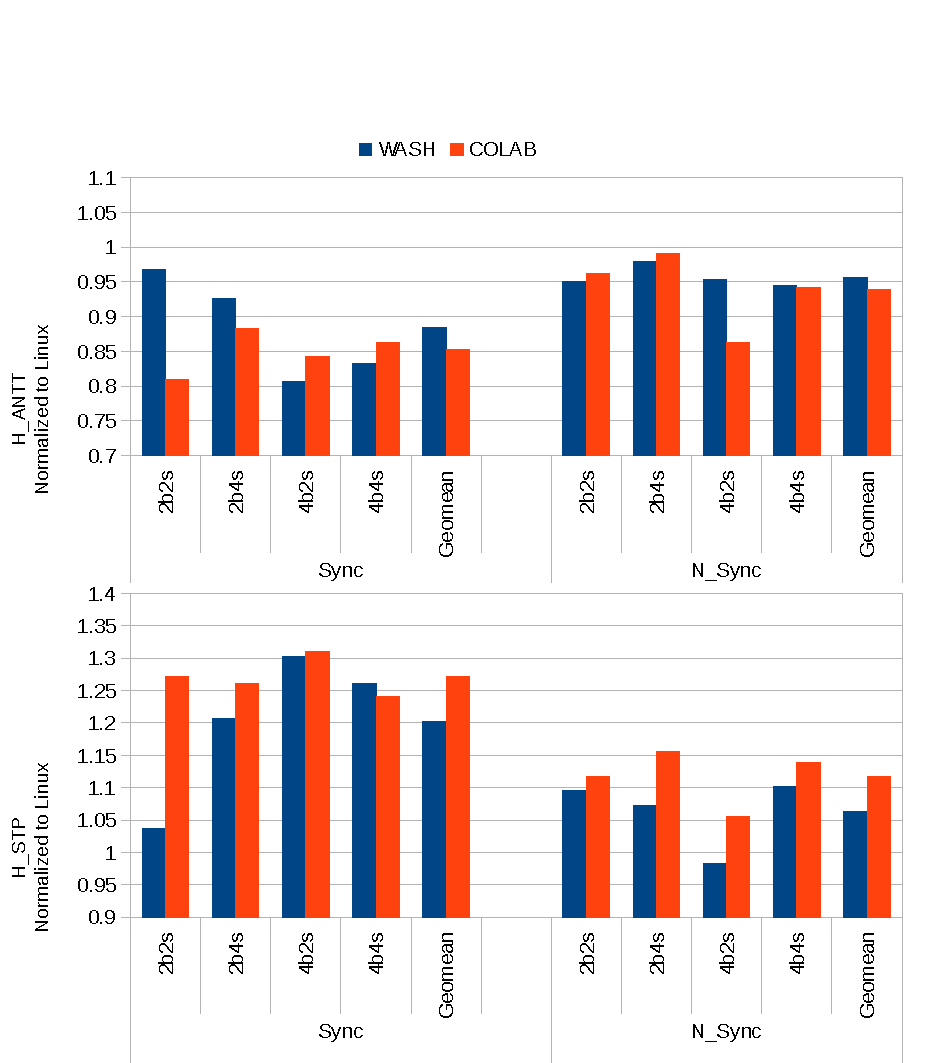
\includegraphics[scale=0.5]{figures/sync.pdf}
%\caption{Heterogeneous Average Normalized Turnaround Time (H\_ANTT) and Heterogeneous System Throughput (H\_STP) of Synchronization-Intensive and Non-Synchronization-Intensive Workloads. All results are normalized to the Linux CFS ones. Lower is better for H\_ANTT and higher is better for H\_STP.}
%\label{sync}
%\end{figure} 

%\paragraph{Synchronisation Intensive vs. Synchronisation Nonintensive Workloads} Figure~\ref{sync} shows the performances of all three schedulers on synchronization-intensive (\emph{Sync}) and synchronization-nonintensive (\emph{N\_Sync}) workloads. As with the other experiments in this section, the experiments here are grouped based on hardware configuration on which they are executed. We present the mean H\_ANTT and H\_STP over four different workloads.
%%(as shown in Figure~\ref{fig:XX}). Note again that lower H\_ANTT and higher H\_STP translate into higher performance of the scheduler. 
%We can observe that, for synchronisation-intensive workloads, COLAB improves turnaround time by around 15\% and 4\% on average compared to Linux and WASH, respectively. We can also observe that on the hardware configurations with smaller number of cores (2B2S), the COLAB scheduler performs especially well compared to Linux and WASH, improving over Linux by up to 20\% and over WASH by up to 16\%. Because Linux and WASH lack effective solutions to handle multiple threads of several applications accessing limited resources. With increasing  pressure  from  co-executed  applications, properly  balancing  bottleneck  acceleration and core sensitivity across multiple programs using only two big cores becomes difficult. WASH places all bottleneck threads onto the big cores, which results in these threads having to wait for CPU time in busy run queues, ending up with only 3\% of performance improvement over Linux. COLAB handles these bottleneck threads in a more holistic way, improving turnaround time by 20\% and system throughput by 27\%, compared to Linux.

%%Synchronization-intensive workloads fully composed by benchmarks with higher synchronization rates than others, which lead to the  much more importance of multiple bottlenecks and critical threads co-acceleration. Both heterogeneous-aware schedulers can show a significant advantage than Linux CFS on these cases. As a result, COLAB improves turnaround time by around 15\% compared to Linux and around 4\% compared to WASH on average of different configurations and workload compositions. On certain workloads and configuration cases, COLAB can outperform Linux by up to 20\% (2B2S) and outperform WASH by up to 16\% (2B2S). 
%%The state-of-the-art WASH scheduler shows its limitations when used on limited resources (2B2S). With increasing  pressure  from  co-executed  applications, properly  balancing  bottleneck  acceleration and core sensitivity across multiple programs using only two big cores becomes difficult. WASH identifies these bottlenecks and assigns their threads to big cores without further consideration. Instead of accelerating the bottleneck threads, this leads to the bottleneck threads getting stuck waiting for CPU time in busy runqueues. At the same time, non-critical threads enjoy short waiting times on little cores. WASH ends up performing only 3\% better than Linux CFS. COLAB handles bottleneck threads in a more holistic way, improving performance around 19\% for the same scenario.
%Similar results are presented for the system throughput. COLAB outperform Linux by around 27\% and outperform WASH by around 7\%. 

%As for synchronization-nonintensive workloads, neither COLAB nor WASH have a significant optimization space, since there are not enough bottleneck and critical threads that can be accelerated. As a result, both schedulers perform similarly to Linux, with COLAB improving turnaround time and system throughput by around 6\% and 12\% compared to Linux and around 2\% and 5\% compared to WASH. 
%\textbf{VJ: 12\% seems quite significant, though.} 

%\textit{This verifies our hypothesis that heterogeneity-aware schedulers bring more benefit, compared to the Linux scheduler, for workloads that are dominated by synchronisation-intensive programs. Furthermore, the COLAB scheduler notably outperforms the state-of-the-art WASH scheduler on limited-resource hardware configurations.}

%\begin{figure}
%\centering
%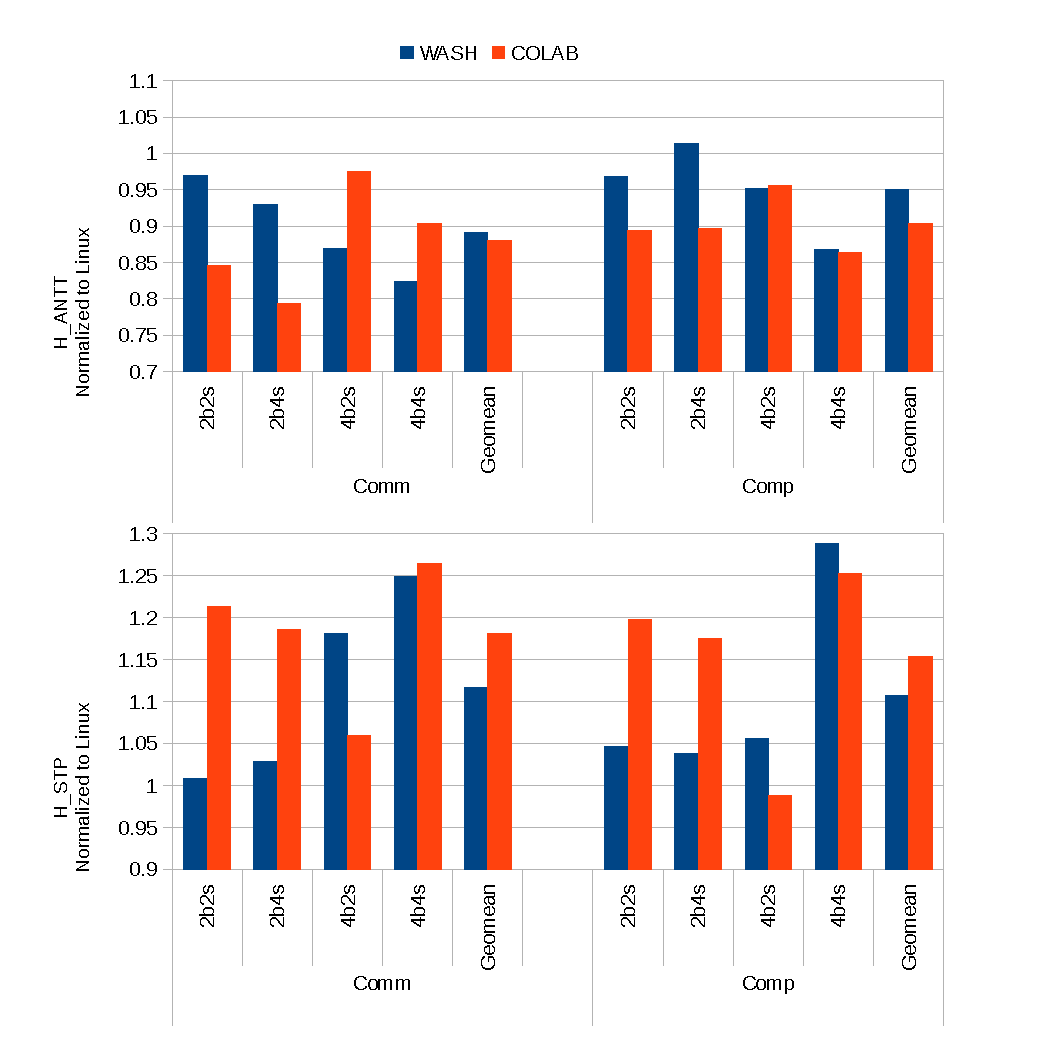
\includegraphics[scale=0.46]{figures/com.pdf}
%\caption{Heterogeneous Average Normalized Turnaround Time (H\_ANTT) and Heterogeneous System Throughput (H\_STP) of Communication-Intensive and Computation-Intensive Workloads. All results are normalized to the Linux CFS ones. Lower is better for H\_ANTT and higher is better for H\_STP.}
%\label{com}
%\end{figure} 

%\begin{figure}
%\centering
%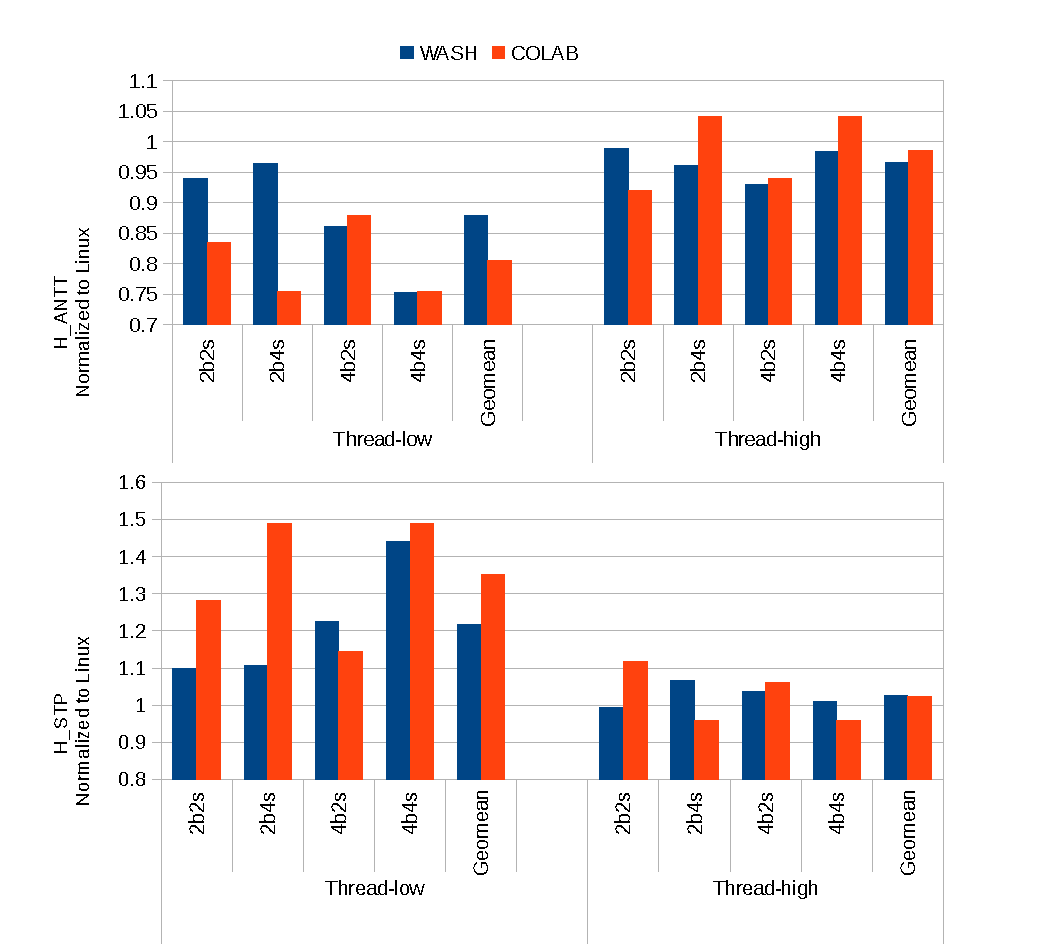
\includegraphics[scale=0.5]{figures/nthread.pdf}
%\caption{Heterogeneous Average Normalized Turnaround Time (H\_ANTT) and Heterogeneous System Throughput (H\_STP) of low number of application threads and high number of application threads Workloads. All results are normalized to the Linux CFS ones. Lower is better for H\_ANTT and higher is better for H\_STP.}
%\label{nthread}
%\end{figure} 

%\paragraph{Communication-intensive vs. Computation-intensive Workloads} Figure~\ref{com} shows the performance of COLAB, WASH and Linux schedulers on communication-intensive and computation-intensive workloads. 
%The hardware configuration is indicated on the X-axis of each subplot. Lower H\_ANTT and higher H\_STP translates into higher performance.
%Communication intensive workloads fully composed by benchmarks with high communication-to-computation ratio, which lead to a significant amount of intra-program communications between multiple application threads. This can result in not only multiple runtime bottlenecks, but also light computation of each thread. So multiple bottlenecks need to be co-executed and each of them has lighter computation need to be done.
%Both COLAB and WASH schedulers improve the Linux scheduler. They, however, offer different advantages on different hardware configurations. COLAB distributes the bottleneck threads to both big and little cores, which results in more significant improvements on limited big-core cases (2B2S, 2B4S). COLAB improves the turnaround time by up to 21\% compared to Linux and 15\% compared to COLAB on the 2B4S configuration. As is the case with the synchronisation-intensive workloads, WASH accumulates the bottleneck threads on big cores only, which results in a better performance where there are enough big-core cases (4B2S, 4B4S). On these configurations, WASH improves turnaround time by up to 18\% over Linux (on 4B4S configuration) and up to 10\% over COLAB (on 4B2S configuration). On average, COLAB improves the turnaround time by around 12\% compared to Linux and 1\% compared to WASH for the communication intensive workloads on all configurations. We observe similar results for system throughput, where COLAB outperforms Linux by around 18\% and outperforms WASH by around 5\%.

%As noted before, computation-intensive workloads offer less improvement space for both heterogeneity-aware schedulers over Limux. Still, we can observe better performance for COLAB than for WASH and Linux, with COLAB improving turnaround time and system throughput by around 10\% and 15\%, respectively, compared to Linux and 5\% compared to WASH. This is, again, due to a fact that multiple bottlenecks are distributed both to big and little cores, which results in more efficient use of the available hardware resources for the few bottlenecks that are present.

%\emph{To summarise, heterogeneous aware schedulers show better performance gain on communication-intensive workloads than on computation-intensive workloads. COLAB outperforms WASH on both workloads on average and shows more significant advantage on computation-intensive workloads. WASH only outperforms COLAB on communication-intensive workloads when there are enough high performance big cores available.}
%%up to 36\% (Comm-4 on 2B2S) and outperform WASH by up tp 24\% (Comm-3 on 2B4S) on turnaround time.



%\begin{figure}
%\centering
%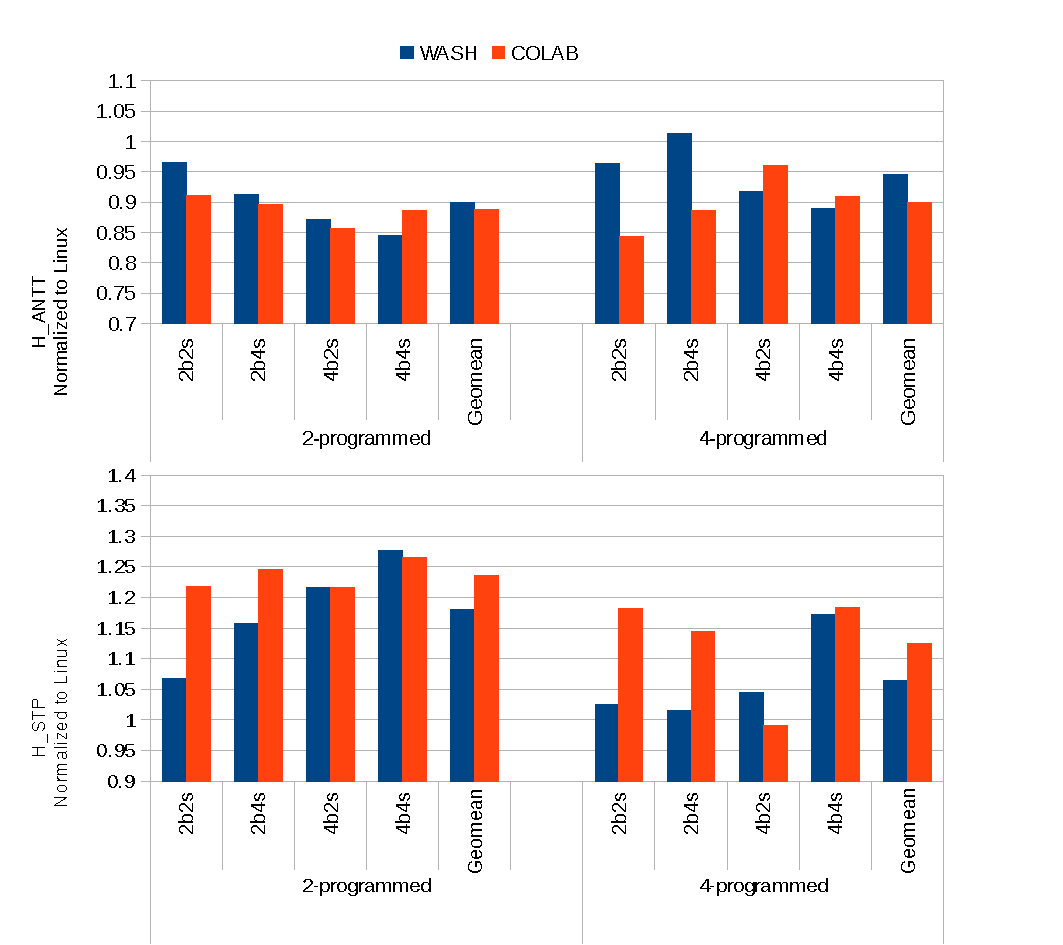
\includegraphics[scale=0.5]{figures/nprog.pdf}
%\caption{Heterogeneous Average Normalized Turnaround Time (H\_ANTT) and Heterogeneous System Throughput (H\_STP) of 2-programmed and 4-programmed Workloads. All results are normalized to the Linux CFS ones. Lower is better for H\_ANTT and higher is better for H\_STP.}
%\label{nprog}
%\end{figure} 

%\begin{figure*}
%\centering
%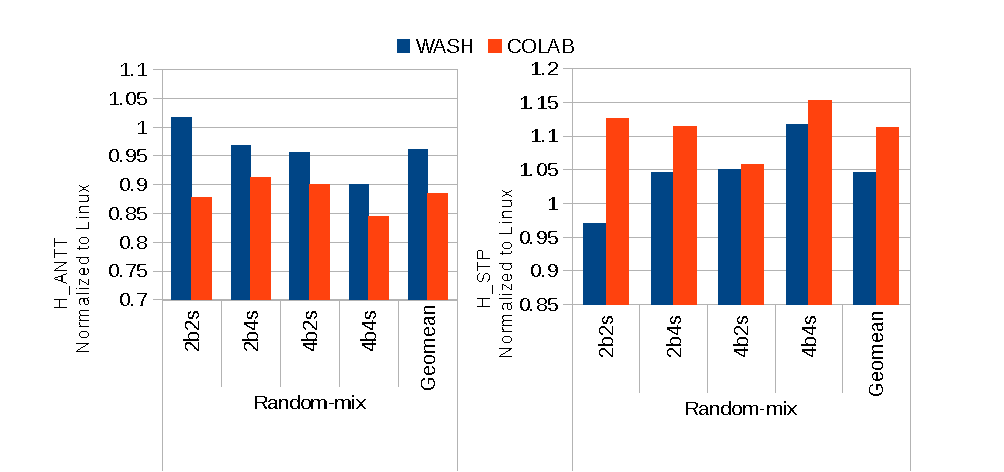
\includegraphics[scale=0.5]{figures/rand.png}
%\caption{Heterogeneous Average Normalized Turnaround Time (H\_ANTT) and Heterogeneous System Throughput (H\_STP) of 2-programmed and 4-programmed Workloads. All results are normalized to the Linux CFS ones. Lower is better for H\_ANTT and higher is better for H\_STP.}
%\label{rand}
%\end{figure*} 

%\paragraph{Mixed Workloads}
%Figure~\ref{rand} shows the performances of 10 mixed workloads. We can observe that COLAB performs very well for these workloads: more diverse programs mean more asymmetry, more bottlenecks, more type of critical threads and more potential for acceleration. Our collaborative multi-factor scheduler carefully handling all the issues (core sensitivity, thread criticality and fairness) brings a significant performance gain against WASH and Linux on this scenario - COLAB improves turnaround time and system throughput by around 12\% and 11\% compared to Linux and around 8\% and 7\% compared to WASH.

%\paragraph{Thread and program count} In our next set of experiments, we studied what impact does the total number of threads and a total number of programs in a workload has on the performance of heterogeneity-aware schedulers. Figure~\ref{nthread} shows the performance of all considered schedulers both for workloads comprising a low number of threads (where there is less threads than cores in the system) and for workloads comprising a high number of threads (where there are significantly more threads than cores). We can observe that both COLAB and WASH perform significantly better than Linux for workloads with a low number of threads. Fewer threads make it easier to indicate the bottlenecks and critical threads, and then to place them carefully on the appropriate resources - either by migrating them to big cores (WASH and COLAB) or by also giving high priorities to them on little cores (COLAB). With limited big core resources, COLAB does enjoy a more significant performance gain against WASH by distributing those few bottlenecks on both big and little cores to accelerate simultaneously and avoid leaving cores idle. COLAB outperforms Linux by up to 25\% (2B4S) and WASH by up to 21\% (2B4S) on turnaround time. On average, COLAB improves turnaround time and system throughput by around 20\% and 35\% compared to Linux and around 8\% and 11\% compared to WASH for workloads with a low number of threads. For workloads with a high number of threads, neither Linux nor WASH are able to improve much on Linux. Overloading the system with threads means that, regardless of where we place threads, cores will have long runqueues. Furthermore, COLAB and WASH do more context switching (due to migration of threads between runqueues), which in this brings significant penalty that cannot be mitigated with good placement of threads. Of the two heterogeneity-aware schedulers, COLAB, with its scale-slice technique, more frequently migrates threads, which results in a slightly worse performance than WASH. On average, COLAB improves turnaround time and system throughput by less than 2\% and 3\% compared to Linux, while WASH slightly outperforms COLAB by 2\% on turnaround time and 0.2\% on system throughput.

%\emph{To summarise this set of experiments, heterogeneity-aware schedulers offer significant advantage over Linux on workloads where the number of threads is approximately the same as the number of cores, with COLAB having much better performance than WASH. When the number of threads in workload is significantly higher than the number of available cores, both scheduler perform similarly to Linux with WASH performing slightly better than COLAB.}

%\textbf{\textit{Number of Co-executed Programs:}}
%The above results are confirmed when we considered workloads with different number of programs in them. Figure~\ref{nprog} shows the performance of all schedulers for 2-programmed and 4-programmed workloads. We can make similar observations as in the case of workloads with variable number of threads - increasing the number of co-executed programs gives higher pressure on the scheduler, increasing the waiting time of threads in runqueues and reducing the direct benefit of migration between waiting threads. But more programs also case more bottlenecks and provide new opportunities for co-acceleration instead of only increasing data-parallel threads. 
%. Heterogeneous aware schedulers generally enjoy better performance gain against Linux on workloads with less programs. Similar as the issue in the above comparisons for total number of threads, more programs with more threads increase the waiting list on runqueues and reduce the direct benefit of migrations between waiting programs/threads.
%By intelligent distributed placing bottlenecks from different programs between big and little cores, our COLAB does face less problem than WASH from the pressure of increasing programs. 

%As a result, both COLAB and WASH outperform Linux by more than 10\% on 2-programmed workloads on turnaround time and COLAB can keep the 10\% performance gain also on 4-programmed workloads, while WASH reduced to only have 5\% performance gain on 4-programmed workloads. As for system throughput, COLAB improves by 23\% and 12\% on 2-programmed and 4-programmed workloads compared to Linux while improves by 5\% and 6\% on 2-programmed and 4-programmed workloads compared to WASH. 
%\textbf{VJ: This is a bit counterintuitive. Why do we get better results for COLAB scheduler when we have more programs but not when we have more threads in a workload?}

\begin{figure*}
\centering
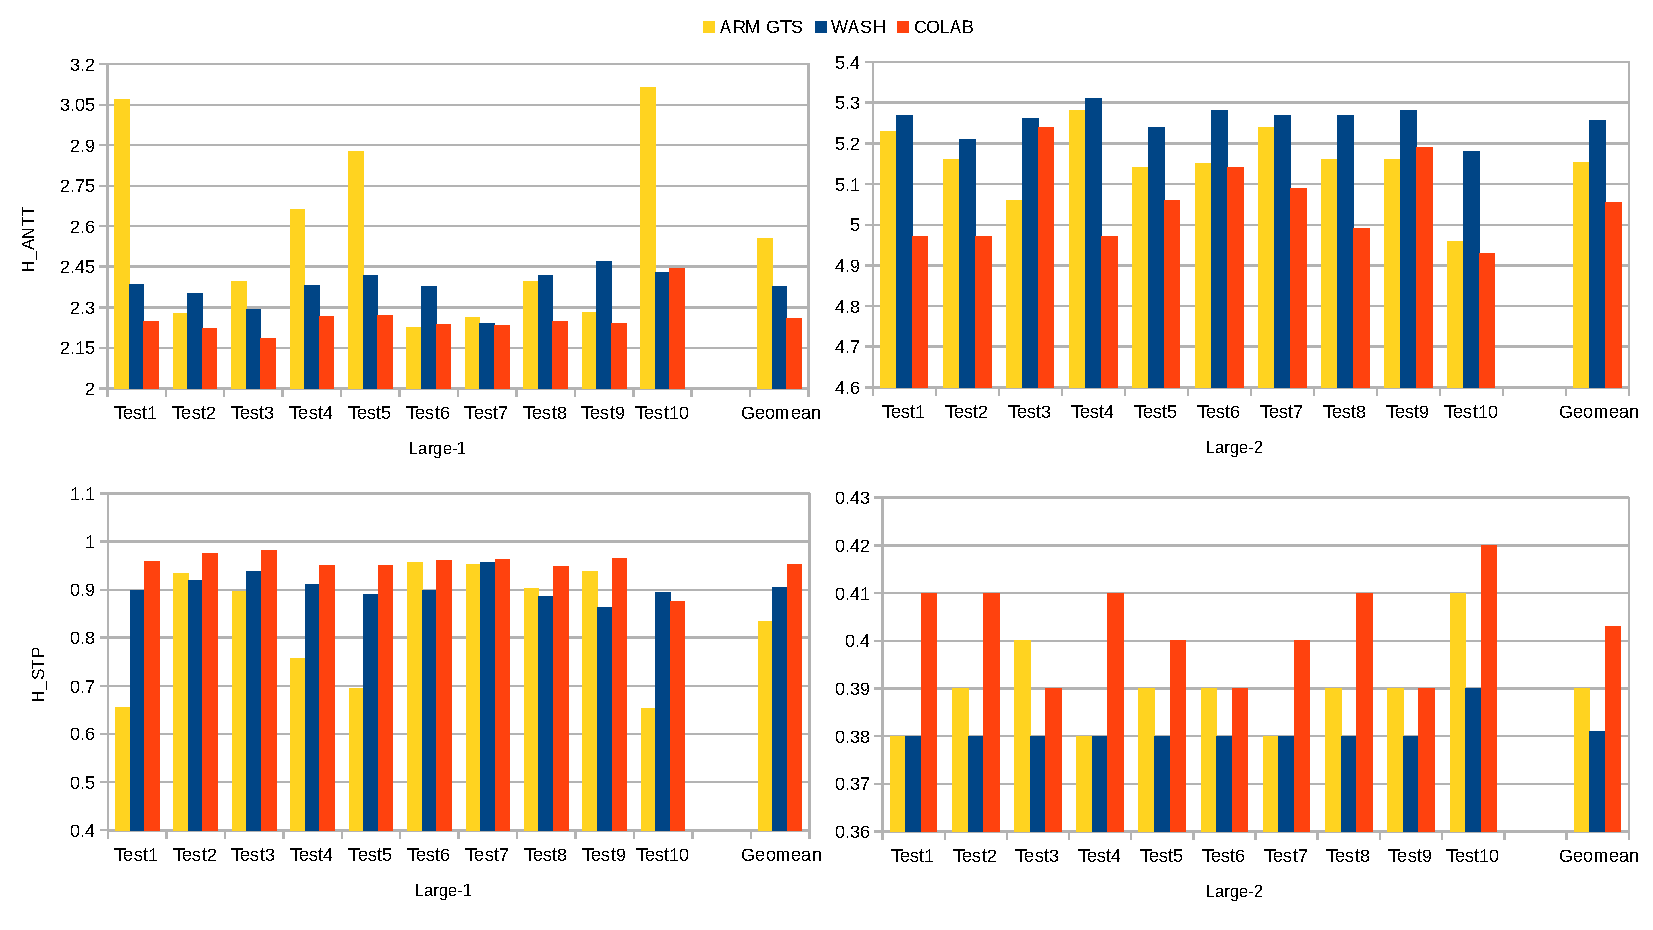
\includegraphics[scale=0.6]{figures/1b1s.pdf}
\caption{Performance of the Large-1 (radix+ocean\_cp) and the Large-2 (ferret+swaptions) workloads using 1 Cortex-A73 core and 1 Cortex-A53 core. Detailed original results from 10 tests with the same 1b1s configuration are presented to show performance variance of ARM GTS scheduler on the real chip. Lower is better for H\_ANTT and higher is better for H\_STP.}
\label{1b1s}
\end{figure*}

\begin{figure}
\centering
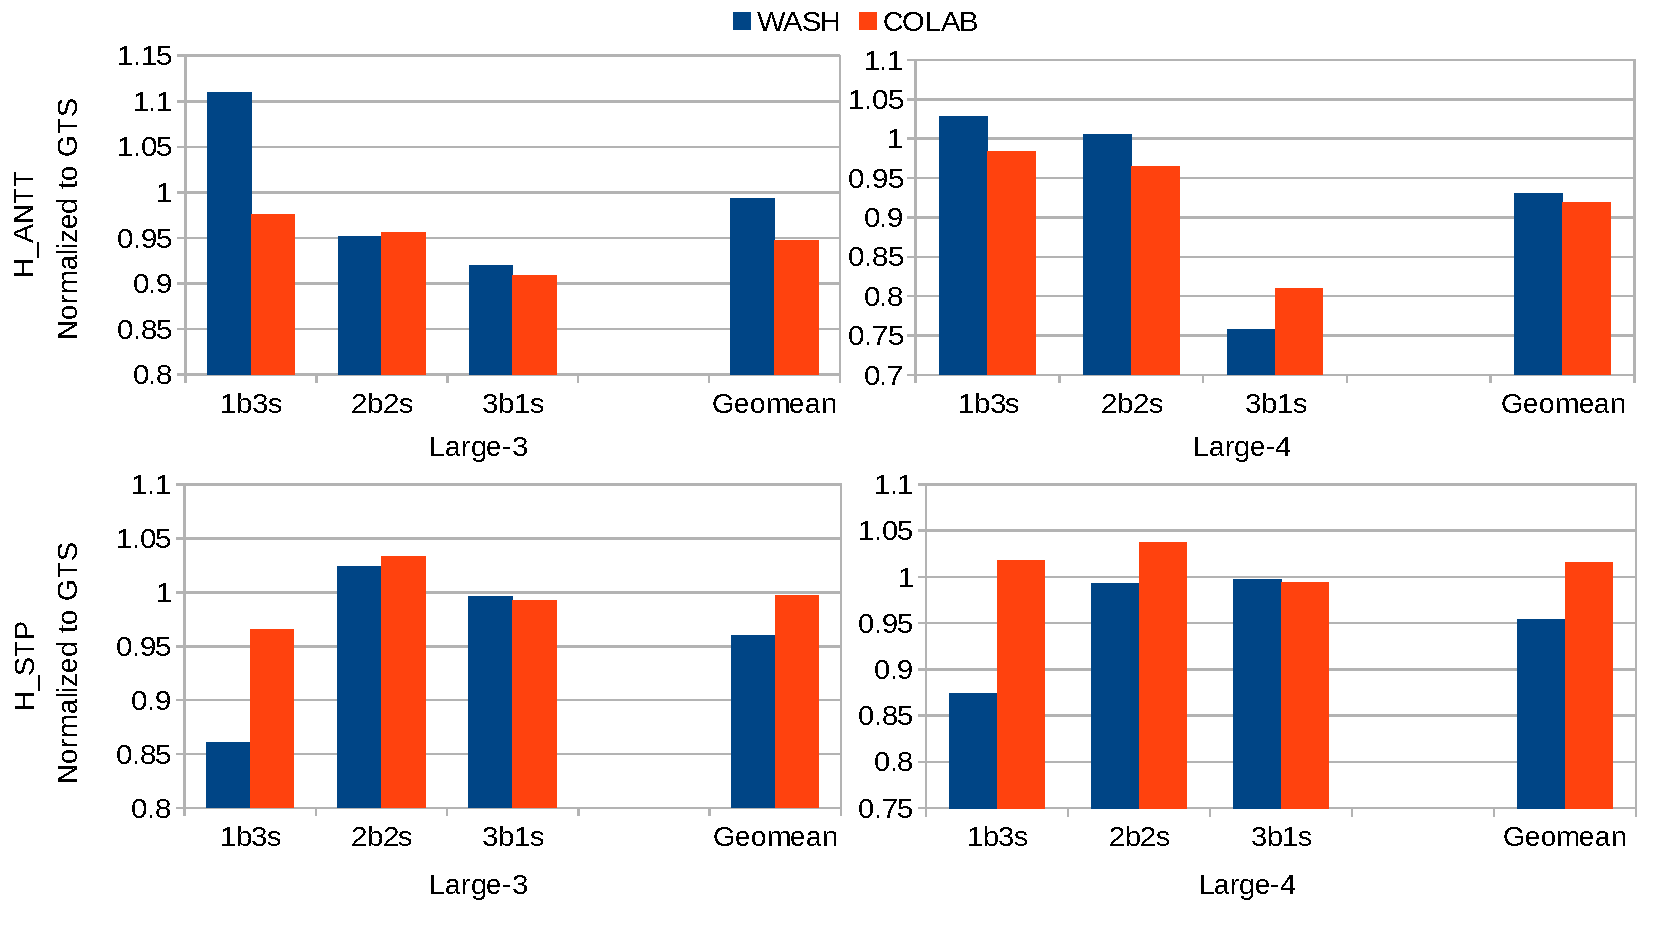
\includegraphics[scale=0.32]{figures/4core.pdf}
\caption{Performance of Large-3 (blackscholes + radix + fluidanimate + water\_spatial) and Large-4 (ocean\_cp + ferret + lu\_cb + swaptions) Workloads using different 4-core configurations. All results are normalized to the ARM GTS ones. Lower is better for H\_ANTT and higher is better for H\_STP.}
\label{4core}
\end{figure}

\begin{figure}
\centering
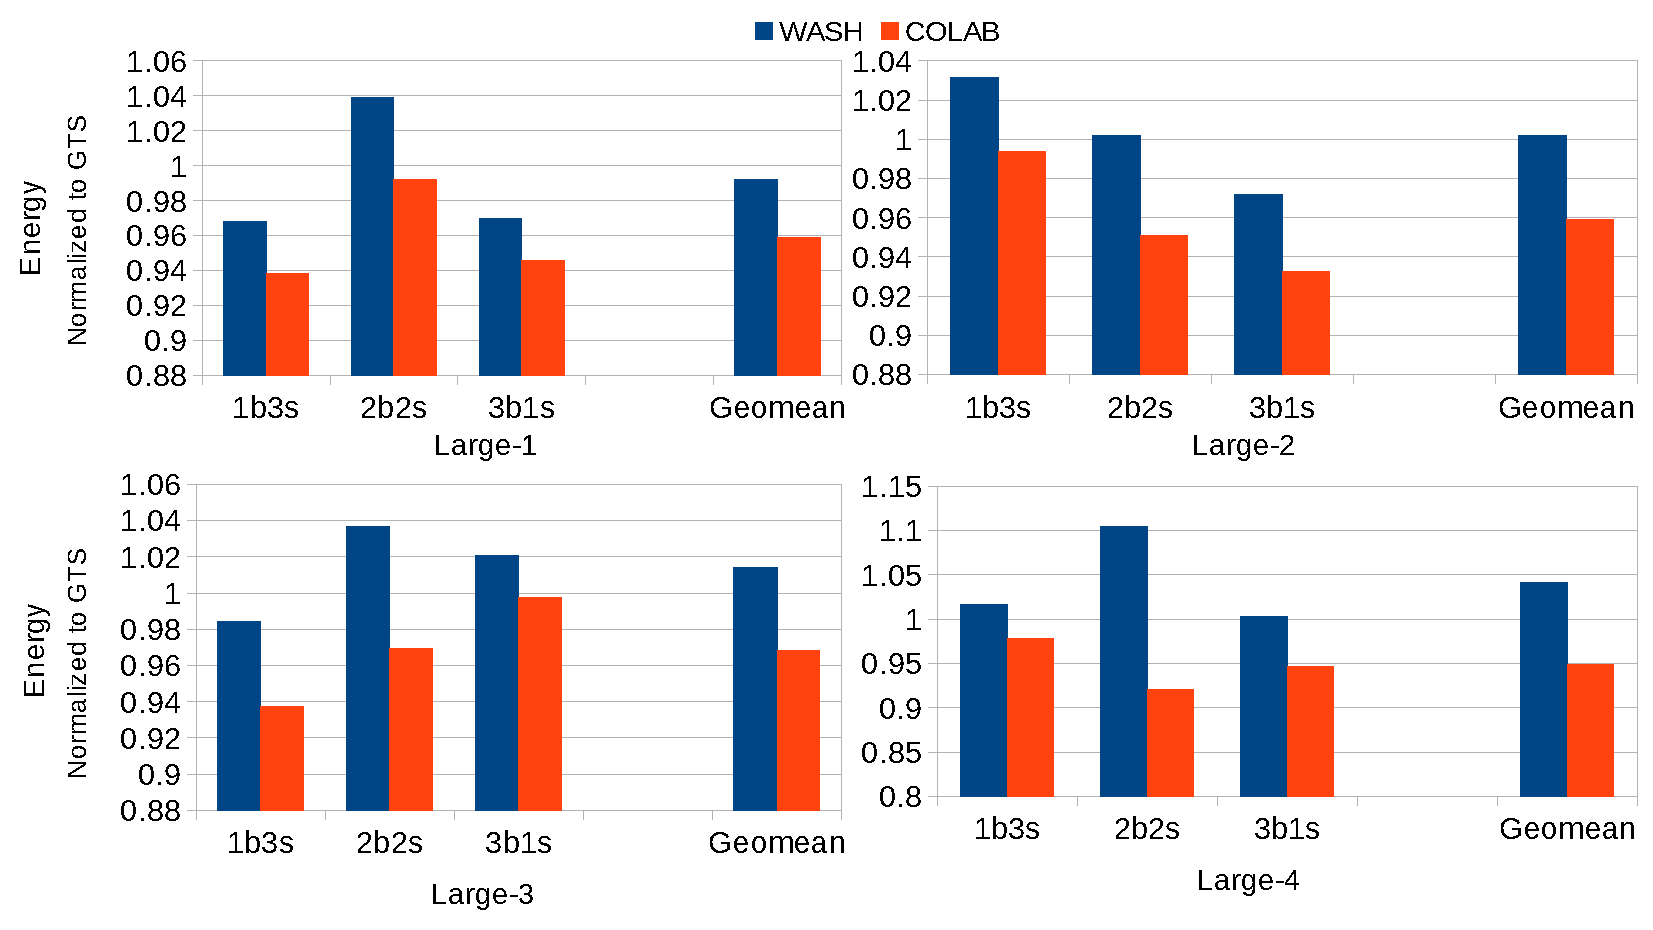
\includegraphics[scale=0.32]{figures/energy_eva.pdf}
\caption{Energy consumption of large multi-programmed Workloads using different 4-core configurations. All results are normalized to the ARM GTS ones. Lower is better for energy.}
\label{elarge}
\end{figure}

\subsection{Experiments on HiHope Hikey 970}
In this section, we validate the performance and the energy efficiency of COLAB with energy-aware extension under large ($simlarge$) mixed multi-threaded multi-programmed workloads on the real ARM big.LITTLE architecture using a HiHope Hikey 970 development board. 
%There is only 4 big cores and 4 little cores in total in the chip. Because we need the baseline performance produced by the fully-big-core configuration, we can only experiment under 2B2S configuration on this development board. The each experiment on real board only take several seconds for $simlarge$ inputs, we can test much large workloads on the board compared with simulation. 

\textbf{\textit{Portable performance on large mixed workloads:}}
Performance variance is significant under the default Linux scheduler (with ARM GTS enable) on the real board compared to checkpoint-based GEM5 simulation. CFS-based ARM GTS scheduler without a core sensitivity aware technique might randomly allocate a high big core speedup thread on either a  big core or a little core.  While WASH and COLAB could make their intelligent decisions if there is a detected high big core speedup thread during runtime. To validate this portable performance, we report performance from 10 tests on two distinct large workloads using a basic 1B1S configuration and then the give the Geo-mean result. 

As shown in the left hand side of Figure~\ref{1b1s}, H\_ANTT results on the Large-1 (radix+ocean\_cp) worklaod for ARM GTS are variant significantly from 2.2 (Test5) to 3.1 (Test10). While for both WASH and COLAB, the H\_ANTT results keep between 2.15 and 2.45. Similar with the results for H\_STP. The Large-1 is a representative mixed workload compared by a high core sensitivity program, ocean\_cp and a low core sensitivity program, radix. The actual speedup between big and little core for ocean\_cp is more than 5x as validated in the performance modelling section. So if ARM GTS unfortunately allocates the high big core speedup threads from ocean\_cp onto the little (Test1, Test4, Test5 and Test10) during execution, COLAB will result in a up-to 27\% (Test10) performance gain compared to ARM GTS. In average, COLAB results in 12\% and 14\% performance gain on H\_ANTT and H\_STP compared to ARM GTS, respectively. WASH can also make kinds of intelligent decisions on keeping the high big core speedup threads from ocean\_cp on the big core. But it will also schedule bottleneck threads from radix, which do not have a good speedup, to occupy the limited big core resources. As a result, COLAB can outperform WASH with an average 5\% performance gain in this workload.

While the main problem of WASH appears when the workload is not core sensitivity as shown in the right hand side of Figre~\ref{1b1s}. Large-2 workload is composed by ferret and swaptions, application threads from both of them don't have significant speedup between big cores and little cores. While, ferret is a synchronization-intensive parallel program which means there will be bottleneck threads during runtime. WASH simply schedules these bottleneck threads to accumulate runqueue of the big core, which can not actually achieve acceleration but make additional system overhead. COLAB shows its unique advantage in this case by in-place accelerate the bottleneck threads on local cores. As a result, COLAB achieves a up-to 6\% (2\% in average) performance gain while WASH suffers a up-to 4.5\% (2\% in average) slowdown on H\_ANTT compared to ARM GTS. The difference is larger for H\_STP, where COLAB achieves a up-to 8\% (3\% in average) performance gain while WASH suffers a up-to 5\% (2\% in average) slowdown compared to ARM GTS.

To further validate the performance of COLAB on general cases, we test two larger workloads (Large-3, Large-4) each composed by 4 programs using distinct 4-core configurations (1B3S, 2B2S and 3B1S). The results are shown in Figure~\ref{4core}, where each bar is the average value of multiple tests by a certain configuration. Similar with the results from GEM5 simulation, COLAB shows its best advantage against WASH on limited big core resource (1B3S). When there is only 1 big core, the bottleneck in-place acceleration technique of COLAB make its intelligent decisions and results in a up-to 12\% (Large-3) performance gain on H\_ANTT compared with WASH. When there are more big core resources, both WASH and COLAB show more advantage as there will be more opportunities to accelerate the needed threads on big cores under core sensitivity aware solutions than CFS-based ARM GTS. For example, WASH and COLAB achieve 24\% and 20\% performance gain on H\_ANTT when running Large-4 on 3B1S configuration compared to ARM GTS. WASH even do better than COLAB as the amount of big cores is sufficient to accelerate both the high speedup and bottleneck threads for the given workload. In average, COLAB achieves 5\%-9\% and 3\%-6\% performance gain on H\_ANTT on the large workloads compared to ARM GTS and WASH, respectively. WASH can not outperform ARM GTS on H\_STP in average based on the problematic scheduling decisions on the 1B3S configuration, while COLAB can still keep good performance.

\textbf{\textit{Energy efficiency on large mixed workloads:}}
%We first test the original COLAB scheduler compared with WASH for performance validation. Then we test the energy-aware COLAB extension for both performance and energy consumption. The default scheduler on the HiHope Hikey 970 board is ARM GTS instead of Linux CFS.
%Figure~\ref{1b1s} shows the performance for these large workloads scheduled by COLAB and WASH against ARM GTS.
Figure~\ref{elarge} shows the performance energy consumption results for large workloads scheduled by COLAB extension and WASH against ARM GTS. In Figure~\ref{elarge}, WASH shows up-to 5\%(Large-4) energy cost. When allocating tasks, WASH simply schedules bottleneck threads to the big core, regardless of how much energy they consume. An application might cost more energy when running in the big core. For ARM GTS, it cannot be aware of energy consumption of tasks. So its result is not very stable and in some cases (Large-1 2B2S and Large-2 1B3S), ARM GTS can outperform WASH with nearly 2\%. 
However, the energy-aware COLAB scheduler takes the advantages of its energy model, uses the predicted energy and allocates each application to proper cores to decrease the consumption. For example, with 1B3S configure, WASH tries to allocate tasks to the big core, which makes the full use of it. But it cost more energy because many tasks are pushed into the run queue of big core. For COLAB, it makes more intelligent decision by considering the energy consumption and schedule those energy-intensive task to little cores in order to reduce the energy consumption.

As shown in Figure-\ref{elarge}, COLAB outperforms ARM GTS and WASH with an average 5\% (up-to 8\%) energy saving in all the large mixed multi-programmed workloads on distinct 4-core based configurations.

%\ty{Figure~\ref{elarge} shows the energy consumption results for these large workloads scheduled by COLAB extension and WASH against ARM GTS.}

%\textbf{\textit{Summary of Experiments:}} Our experiments showed that the state-of-the-art heterogeneous-aware WASH scheduler struggles to make better scheduling decisions that the Linux schedules for synchronization-intensive workloads, computation-intensive workloads, low threads number workloads, high program number workloads, mixed multi-class workloads and limited big cores configurations. Trying to handle both core sensitivity, bottleneck acceleration and fairness through thread affinity alone may lead to too many threads assigned to big cores. Instead, we assign on big cores only threads which run significantly faster on them and we prioritize running bottleneck threads regardless of their thread affinity. This leads to improved turnaround time, higher throughput, and better use of the processor resources compared to both Linux and WASH. In summary from all 312 experiments, COLAB improves turnaround time and system throughput by 11\% and 15\% compared to Linux and by 5\% and 6\% compared to WASH. \vspace{-1em}
%COLAB improves performance by up to 25\% and 21\% lower trunaround time, 11\% and 5\% on average, compared to Linux CFS and WASH scheduler.


%\begin{table*}
 % \caption{Workloads Compositions}
 % \center
 % \label{WC}
 %  \scalebox{0.9}{
 %  \begin{tabular}{p{1.5cm} |p{5.5cm} || p{1.5cm} |p{9cm} }
 %    \toprule[1pt]
 %    \multicolumn{4}{c}{Random-mixed Workloads from PARSEC3.0 and SPLASH-2}\\
 %    \toprule[1pt] 
 %   2B-1 &blackshcoles - radix &4B-1 &blackshcoles - bodytrack - radix - lu\_ncb\\
 %   2B-2 &fft - swaptions &4B-2 &water\_spatial - fmm - fft - fluidanimate\\
 %   2B-3 &lu\_cb - dedup  &4B-3 &lu\_cb - water\_nsquared - fmm - freqmine\\
 %   2B-4 &lu\_ncb - bodytrack &4B-4 &lu\_cb - lu\_ncb - bodytrack - dedup\\
 %  2B-5 &ferret - fluidanimate &4B-5 &radix - lu\_ncb - lu\_cb - fft\\
  %  2B-6 &freqmine - water\_nsquared &4B-6 &blackscholes - bodytrack - dedup - fluidanimate\\
  %  2B-7 &ocean\_cp - fft &4B-7 &radix - ocean\_cp - blackscholes - swaptions\\
  %  2B-8 &ferret - water\_spatial &4B-8 &water\_spatial - water\_nsquared - ferret - freqmine\\
  %  2B-9 &fluidanmiate - fmm &4B-9 &fmm - water\_spatial - ferret - swaptions\\
  %  2B-10 &fmm - water\_spatial &4B-10 &ocean\_cp - fft - fluidanimate - swaptions\\
  %  6B-M &blackshcoles,bodytrack,dedup,radix,lu\_ncb,lu\_cb\\
  %  8B-M &blackshcoles,bodytrack,dedup,fluidanmiate,radix,lu\_ncb,lu\_cb,radiosity\\
  %  12B-M &blackshcoles,bodytrack,dedup,fluidanmiate,streamcluster,swaptions,radix,lu\_ncb,lu\_cb,radiosity,ocean\_cp,fft\\    
%     \midrule
 %    \toprule[1pt]
 %    \multicolumn{4}{c}{Multi/Single-thread multiprogrammed Workloads from PARSEC3.0, SPLASH-2 and SPEC2006}\\
 %    \toprule[1pt]  
 %   3B-1 &blackshcoles - radix - mcf &6B-1 &blackshcoles - bodytrack - radix - lu\_ncb - mcf - bzip2\\
  %  3B-2 &fft - swaptions - mcf &6B-2 &fft - radix - blackscholes - fluidanimate - mcf - bzip2\\
   % 3B-3 &freqmine - swaptions - mcf &6B-3 &blackscholes - dedup - freqmine - swaptions - mcf - bzip2\\
%    3B-4 &blackscholes - freqmine - bzip2 &6B-4 &lu\_cb - lu\_ncb - bodytrack - dedup - mcf - bzip2\\
    %3B-5 &ocean\_cp - fluidanimate - mcf &6B-5 &radix - lu\_ncb - lu\_cb - fft - mcf - bzip2\\
 %   3B-5 &radix - lu\_ncb - bzip2 &6B-5 &radix - lu\_ncb - lu\_cb - fft - mcf - bzip2\\
  %  3B-6 &fluidanimate - freqmine - bzip2 &6B-6 &blackscholes - freqmine - swaptions - fluidanimate - mcf - bzip2\\
   % 3B-7 &blackscholes - fluidanimate - bzip2 &6B-7 &lu\_ncb - ocean\_cp - bodytrack - swaptions - mcf - bzip2\\
%    3B-8 &dedup - fluidanimate - bzip2 &6B-8 &lu\_cb - ocean\_cp - dedup - swaptions - mcf - bzip2\\
 %   3B-9 &lu\_cb - swaptions - bzip2 &6B-9 &ocean\_cp - fft - fluidanimate - swaptions - mcf - bzip2\\
 %   7B-MS   &blackshcoles,bodytrack,dedup,radix,lu\_ncb,lu\_cb,mcf\\
 %   11B-MS &blackshcoles,bodytrack,dedup,canneal,swaptions,radix,lu\_ncb,lu\_cb,radiosity, bzip2,mcf\\ 
  %  15B-MS &blackshcoles,bodytrack,dedup,fluidanmiate,streamcluster,canneal,swaptions,radix,lu\_ncb,lu\_cb,radiosity, ocean\_cp,fft,bzip2,mcf\\   
  % &6B-7 &radix - ocean\_cp - blackscholes - swaptions - mcf - bzip2\\
 %   \bottomrule
 % \end{tabular}}
%\end{table*}

\vspace{-0.1cm}
\section{Conclusion}

We presented the novel \textbf{COLAB} scheduling framework that targets multi-threaded multiprogrammed workloads on asymmetric multicore processors (AMPs) which occupy a significant part of the processor market today, especially in embedded systems. COLAB is the first general-purpose scheduler that, by making \emph{collaborative} decisions on core sensitivity, thread criticallity and scheduling fairness, optimises all these three factors that affect the AMP scheduling - core affinity, thread criticality, and scheduling fairness. %In this way, we are able to improve on the state-of-the art WASH scheduler, as well as on the Linux CFS scheduler.
%, which consider these two decisions in isolation. 

We have demonstrated on a number of different workloads comprised of benchmarks taken from the state-of-the-art parallel benchmark suites PARSEC3.0 and SPLASH-2, simulating a number of different AMP configurations using the well-known GEM5 simulator and then testing on a ARMv8-based HiHope Hikey 970 development board, that the COLAB scheduler outperforms state-of-the-art WASH, ARM GTS and Linux CFS schedulers by up to 21\%, 20\% and 25\%, respectively, in terms of turnaround time (5\%, 9\% and 11\% on the average).
We also demonstrate improvements of 6\%, 2\% and 15\% in terms of system throughput on the average. Finally, we show that COLAB achieves an average 5\% energy saving compared to both WASH and ARM GTS. This demonstrates the applicability of our approach in realistic scenarios, allowing better execution times and energy efficiency for parallel workloads on AMP processors without additional effort from the programmer.

This work is extended from the previous work published in CGO 2020~\cite{teng_colab_cgo2020}.



%\IEEEraisesectionheading{\section{Introduction}\label{sec:introduction}}

\bibliographystyle{plain}
\bibliography{sample-base.bib}

%\vskip -1\baselineskip plus -1fil
\begin{IEEEbiography}[{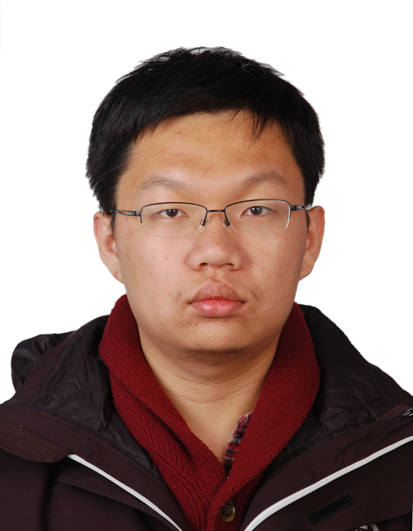
\includegraphics[width=0.95in,height=1.25in,clip,keepaspectratio]{./photo/ty.jpg}}]{Teng Yu \textnormal{is a PostDoctoral Researcher at the Department of Computer Science and Technology, Tsinghua University. He received his PhD degree from University of St Andrews in 2020. His research interests include operating systems, heterogeneous architectures and HPC.}}
\end{IEEEbiography}
\vskip -1\baselineskip plus -1fil
%\vspace{-1em}
\begin{IEEEbiography}[{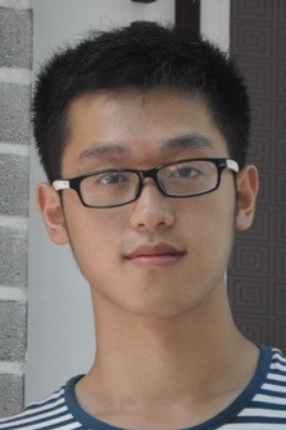
\includegraphics[width=0.95in,height=1.15in,clip,keepaspectratio]{./photo/rz.png}}]{Runxin Zhong \textnormal{is an 3rd year undergraduate student at the Department of Computer Science and Technology, Tsinghua University. His research interest is quantum computation and HPC.}}
\end{IEEEbiography}
\vskip -1\baselineskip plus -1fil
\begin{IEEEbiography}[{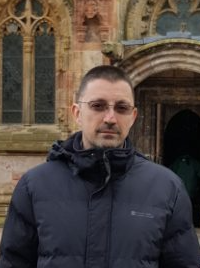
\includegraphics[width=0.95in,height=1.10in,clip,keepaspectratio]{./photo/VJ.png}}]{Vladimir Janjic \textnormal{is a Lecturer (Assistant Professor) in the School of Science and Engineering, University of Dundee. His research interests are high-level programming models (based on the concept of parallel patterns) for heterogeneous parallel platforms, as well as efficient implementation of these models on hardware.}}
\end{IEEEbiography}
\vskip -1\baselineskip plus -1fil
\begin{IEEEbiography}[{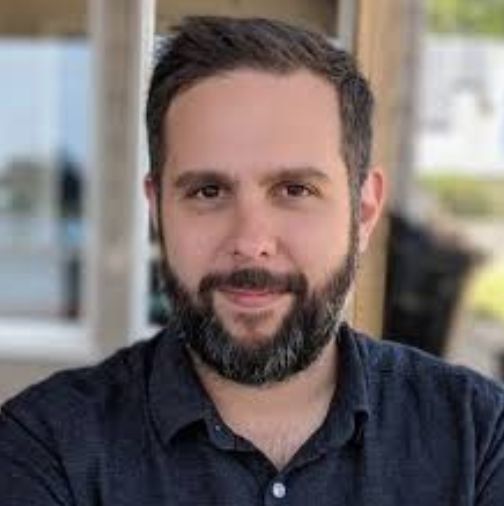
\includegraphics[width=0.95in,height=1.15in,clip,keepaspectratio]{./photo/pp.png}}]{Pavlos Petoumenos \textnormal{is a Lecturer (Assistant Professor) in the Department of Computer Science at the University of Manchester and
a Research Fellow of the Royal Academy of Engineering. His research focuses on compilers, runtime systems, and development tools that help programmers write fast, energy efficient programs with as little effort as possible.}}
\end{IEEEbiography}
\vskip -1\baselineskip plus -1fil
\begin{IEEEbiography}[{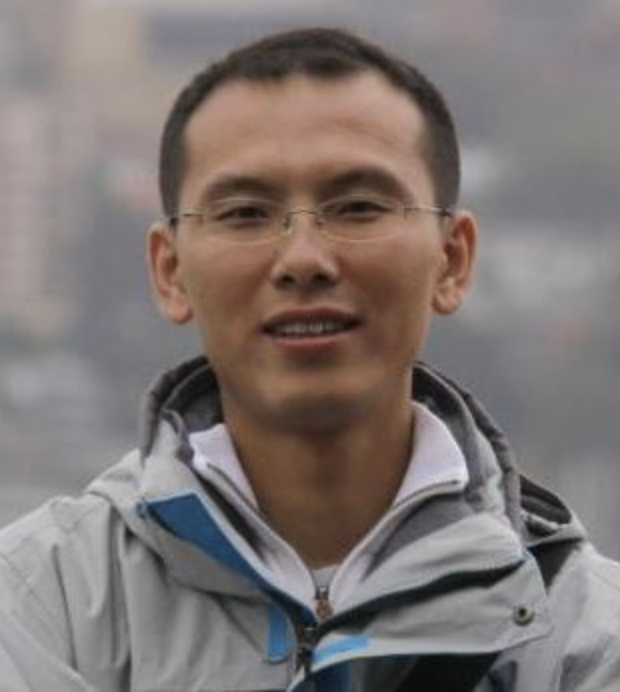
\includegraphics[width=0.95in,height=1.25in,clip,keepaspectratio]{./photo/jz.png}}]{Jidong Zhai \textnormal{is an Associate Professor at the Department of Computer Science and Technology, Tsinghua University. His research focuses on high performance computing, especially performance analysis and optimization for large-scale parallel applications and performance evaluation for computer systems. He received his PhD degree from Tsinghua University in 2010}}
\end{IEEEbiography}
\vskip -1\baselineskip plus -1fil
\begin{IEEEbiography}[{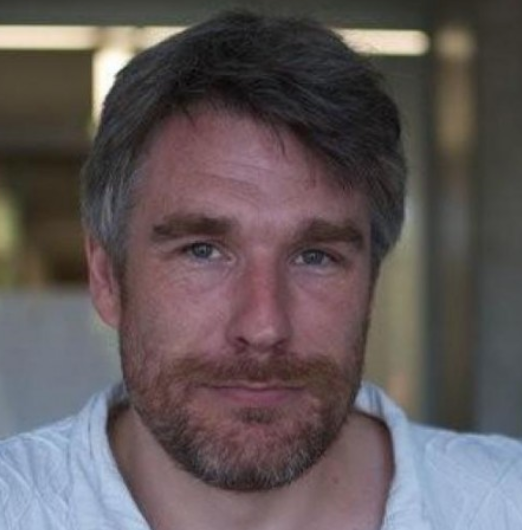
\includegraphics[width=0.95in,height=1.10in,clip,keepaspectratio]{./photo/hl.png}}]{Hugh Leather \textnormal{is a Reader (Associate Professor) in the School of Informatics at the University of Edinburgh. He is a Royal Academy of Engineering / EPSRC Research Fellow. His research is about improving the energy consumption and performance of computers, ranging from mobile systems to data centres.}}
\end{IEEEbiography}
\vskip -1\baselineskip plus -1fil
\begin{IEEEbiography}[{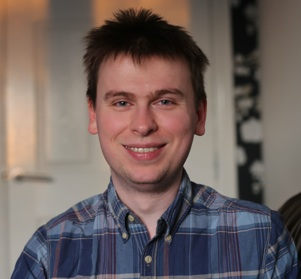
\includegraphics[width=0.95in,height=1.25in,clip,keepaspectratio]{./photo/jt.jpg}}]{John Thomson \textnormal{is a Lecturer (Assistant Professor) in the School of Computer Science, University of St Andrews. John's Research interests center around empirical approaches to systems design, including optimising compilers, video compression, HPC, embedded systems, applied machine learning, parallelisation techniques and runtime systems.}}
\end{IEEEbiography}

\end{document}